\documentclass[oneside,numbers,spanish,nobibtoc]{ezthesis}

\usepackage{tabularx}

% Paquete  que permite  cambiar  el formato  en  el que  se ponen  los
% títulos   de   capítulos,  secciones,   etc.    También  define   el
% comando \chaptertitlename, que  equivale a \chaptername ("Capítulo")
% cuando se está  dentro de un capítulo o  a \apendixname ("Apéndice")
% cuando se  está en un apéndice.  Eso se utiliza en  la definición de
% las cabeceras.
\usepackage{titlesec}
\usepackage{amsfonts,amssymb}
\usepackage{amsmath}
\usepackage{graphicx}
\usepackage{enumerate}
\usepackage[utf8]{inputenc}
%\usepackage[spanish]{babel}
\usepackage{amsthm}
\usepackage{lipsum}
%\usepackage{calligra}
%\usepackage{calrsfs}
\usepackage{mathrsfs}
\usepackage{epstopdf}
\usepackage{subfigure}
%\usepackage{dsfont}
\usepackage{tikz}
\usepackage{filecontents}
%\usepackage{verbatim}
\usepackage{amssymb}
\usepackage[T1]{fontenc}
\usepackage[numbers]{natbib}
\usepackage{multirow}
\usepackage{color}

\theoremstyle{definition}

\newtheorem{definition}{Definición}[chapter] % esto es para que lo numere como : capitulo. definicion


\newcommand*{\id}{{\normalfont\hbox{1\kern-0.15em \vrule width .8pt depth-.5pt}}}

%\renewcommand{\spanishtablename}{Tabla}



\addto\captionsspanish{\renewcommand{\tablename}{Fig.}}

% Definimos  los  nombres para  las  tablas  y  el índice  de  tablas,
% sobreescribiendo los de babel, que los llama 'cuadros'.

%% # Opciones disponibles para el documento #
%%
%% Las opciones con un (*) son las opciones predeterminadas.
%%
%% Modo de compilar:
%%   draft            - borrador con marcas de fecha y sin im'agenes
%%   draftmarks       - borrador con marcas de fecha y con im'agenes
%%   final (*)        - version final de la tesis
%%
%% Tama'no de papel:
%%   letterpaper (*)  - tama'no carta (Am'erica)
%%   a4paper          - tama'no A4    (Europa)
%%
%% Formato de impresi'on:
%%   oneside          - hojas impresas por un solo lado
%%   twoside (*)      - hijas impresas por ambos lados
%%
%% Tama'no de letra:
%%   10pt, 11pt, o 12pt (*)
%%
%% Espaciado entre renglones:
%%   singlespace      - espacio sencillo
%%   onehalfspace (*) - espacio de 1.5
%%   doublespace      - a doble espacio
%%
%% Formato de las referencias bibliogr'aficas:
%%   numbers          - numeradas, p.e. [1]
%%   authoryear (*)   - por autor y a'no, p.e. (Newton, 1997)
%%
%% Opciones adicionales:
%%   spanish         - tesis escrita en espa'nol
%%
%% Desactivar opciones especiales:
%%   nobibtoc   - no incluir la bibiolgraf'ia en el 'Indice general
%%   nofancyhdr - no incluir "fancyhdr" para producir los encabezados
%%   nocolors   - no incluir "xcolor" para producir ligas con colores
%%   nographicx - no incluir "graphicx" para insertar gr'aficos
%%   nonatbib   - no incluir "natbib" para administrar la bibliograf'ia

%% Paquetes adicionales requeridos se pueden agregar tambi'en aqu'i.
%% Por ejemplo:
%\usepackage{subfig}
%\usepackage{multirow}

%% # Datos del documento #
%% Nota que los acentos se deben escribir: \'a, \'e, \'i, etc.
%% La letra n con tilde es: \~n.

\author{Julia Analía Cassetti}
\title{Estimación de Parámetros en Imágenes SAR monopolarizadas Usando Distancias Estocásticas y Núcleos Asimétricos}
\degree{Doctor en Ciencia y Tecnología}
\supervisor{Dr. Alejandro Frery Orgambide}
\institution{Universidad Nacional de General Sarmiento}
%\faculty{Escuela de Ingenier\'ia y Ciencias}
%\department{Departamento de Sistemas Computacionales}

%% # M'argenes del documento #
%% 
%% Quitar el comentario en la siguiente linea para austar los m'argenes del
%% documento. Leer la documentaci'on de "geometry" para m'as informaci'on.

%\geometry{top=40mm,bottom=33mm,inner=40mm,outer=25mm}

%% El siguiente comando agrega ligas activas en el documento para las
%% referencias cruzadas y citas bibliogr'aficas. Tiene que ser *la 'ultima*
%% instrucci'on antes de \begin{document}.
\hyperlinking

\begin{document}

%% En esta secci'on se describe la estructura del documento de la tesis.
%% Consulta los reglamentos de tu universidad para determinar el orden
%% y la cantidad de secciones que debes de incluir.

%% # Portada de la tesis #
%% Mirar el archivo "titlepage.tex" para los detalles.

%% ## Construye tu propia portada ##
%% 
%% Una portada se conforma por una secuencia de "Blocks" que incluyen
%% piezas individuales de informaci'on. Un "Block" puede incluir, por
%% ejemplo, el t'itulo del documento, una im'agen (logotipo de la universidad),
%% el nombre del autor, nombre del supervisor, u cualquier otra pieza de
%% informaci'on.
%%
%% Cada "Block" aparece centrado horizontalmente en la p'agina y,
%% verticalmente, todos los "Blocks" se distruyen de manera uniforme 
%% a lo largo de p'agina.
%%
%% Nota tambi'en que, dentro de un mismo "Block" se pueden cortar
%% lineas usando el comando \\
%%
%% El tama'no del texto dentro de un "Block" se puede modificar usando uno de
%% los comandos:
%%   \small      \LARGE
%%   \large      \huge
%%   \Large      \Huge
%%
%% Y el tipo de letra se puede modificar usando:
%%   \bfseries - negritas
%%   \itshape  - it'alicas
%%   \scshape  - small caps
%%   \slshape  - slanted
%%   \sffamily - sans serif
%%
%% Para producir plantillas generales, la informaci'on que ha sido inclu'ida
%% en el archivo principal "tesis.tex" se puede accesar aqu'i usando:
%%   \insertauthor
%%   \inserttitle
%%   \insertsupervisor
%%   \insertinstitution
%%   \insertdegree
%%   \insertfaculty
%%   \insertdepartment
%%   \insertsubmitdate
\vspace{-3cm}
\begin{flushright}
	\includegraphics[width=0.33\linewidth]{../../Logos/LogoUngs.jpg}
\end{flushright}

\begin{titlepage}
\vspace{-4cm}
\begin{center}
	\textbf{DOCTORADO EN CIENCIA Y TECNOLOGIA}\vspace{-3mm}\\
	\hrulefill\\
	{\small Evaluado y acreditado por la Comisión Nacional de Evaluación y Acreditación Universitaria (CONEAU). \emph{Resolución Nº 1178/11. Calificación “B”}.}
\end{center}

\vspace{1.5cm}

%\pagenumbering{gobble}
\noindent\makebox[\linewidth]{\rule{15 cm}{1.5pt}}
\begin{center}
	\textbf{{\LARGE Estimación de Parámetros en Imágenes SAR Monopolarizadas Usando Distancias Estocásticas y Núcleos Asimétricos}}
\end{center}
\noindent\makebox[\linewidth]{\rule{15 cm}{1.5pt}}

\vspace{1cm}

  %\TitleBlock{\scshape\insertinstitution}
  %\TitleBlock[\bigskip]{\scshape\insertfaculty}
 % \TitleBlock{\Huge\scshape\inserttitle}
  \TitleBlock{\scshape
    {\large Trabajo de tesis para optar por el título de \\
    Doctor en Ciencia y Tecnología de la \\
    Universidad Nacional de General Sarmiento}}

\vspace{2.5cm}

\TitleBlock{\scshape {\large Autor:\textbf{ Julia Analía Cassetti}}}
\vspace{1cm}

\TitleBlock{\scshape {\large Director: Dr. Alejandro Frery Orgambide}}
\vspace{1.5cm}

\TitleBlock{Diciembre 2019}
  %\TitleBlock[\bigskip]{\insertdepartment}
\end{titlepage}

%% Nota 1:
%% Se puede agregar un escudo o logotipo en un "Block" como:
%%   \TitleBlock{\includegraphics[height=4cm]{escudo_uni}}
%% y teniendo un archivo "escudo_uni.pdf", "escudo_uni.png" o "escudo_uni.jpg"
%% en alg'un lugar donde LaTeX lo pueda encontrar.

%% Nota 2:
%% Normalmente, el espacio entre "Blocks" se extiende de modo que el
%% contenido se reparte uniformemente sobre toda la p'agina. Este
%% comportamiento se puede modificar para mantener fijo, por ejemplo, el
%% espacio entre un par de "Blocks". Escribiendo:
%%   \TitleBlock{Bloque 1}
%%   \TitleBlock[\bigskip]{Bloque2}
%% se deja un espacio "grande" y de tama~no fijo entre el bloque 1 y 2.
%% Adem'as de \bigskip est'an tambi'en \smallskip y \medskip. Si necesitas
%% aun m'as control puedes usar tambi'en, por ejemplo, \vspace*{2cm}.




%% # Prefacios #
%% Por cada prefacio (p.e. agradecimientos, resumen, etc.) crear
%% un nuevo archivo e incluirlo aqu'i.
%% Para m'as detalles y un ejemplo mirar el archivo "gracias.tex".

%% Las secciones del "prefacio" inician con el comando \prefacesection{T'itulo}
%% Este tipo de secciones *no* van numeradas, pero s'i aparecen en el 'indice.
%%
%% Si quieres agregar una secci'on que no vaya n'umerada y que *tampoco*
%% aparesca en el 'indice, usa entonces el comando \chapter*{T'itulo}
%%
%% Recuerda que aqu'i ya puedes escribir acentos como: 'a, 'e, 'i, etc.
%% La letra n con tilde es: 'n.

\chapter*{Agradecimientos}

Quiero agradecer especialmente a mi director Dr.\ Alejandro C.\ Frery por su apoyo permanente, su estímulo y su presencia constante a lo largo de estos años. 

A mis amigos Fer y Lía, Pablo y Lore por estar en mi vida y acompañarme en este camino.

A mi amiga Lore por esas caminatas de los viernes que tanto bien me hicieron y me hacen al alma.

A mis amigos Nino y Cristina por compartir la vida y especialmente por estar presentes en cada momento de la realización de esta tesis.

A mis amigos Michel y Alejandra que desde el país vecino siempre estuvieron a mi lado.

A mi amigo Pablo por permitirme tomar una licencia.

A mi compañero de docencia y amigo Gustavo, que tanta catarsis hemos hecho durante este recorrido.

A mis compañeros de oficina Eda y Roberto por acompañarme en este proceso. 

A mi hermana querida por estar siempre.

A mis padres que hubiesen estado muy felices por este logro en mi vida.

Finalmente quiero agradecer profundamente a mi marido Tico, por su presencia constante, su apoyo incondicional, su tiempo dedicado, su amor, por confiar y creer en mí y por\dots\ tanto por decir.

%% # 'Indices y listas de contenido #
%% Quitar los comentarios en las lineas siguientes para obtener listas de
%% figuras y cuadros/tablas.


\renewcommand{\tablename}{Tabla} 
\renewcommand{\listtablename}{Indice de tablas}
\tableofcontents
\listoffigures
\listoftables

%% # Cap'itulos #
%% Por cada cap'itulo hay que crear un nuevo archivo e incluirlo aqu'i.
%% Mirar el archivo "intro.tex" para un ejemplo y recomendaciones para
%% escribir.

\chapter{Resumen}

Las imágenes obtenidas con dispositivos que poseen iluminación coherente como lo son el ultrasonido, laser o radar de apertura sintética, son afectadas por la presencia de un ruido que es inherente al proceso de captura de la imagen, llamado ruido speckle. Este ruido se aparta de las hipótesis clásicas ya que no es gaussiano, no es aditivo y es difícil de eliminar. 

En los últimos años se ha dedicado especial atención al modelado de datos que provienen de imágenes de radares de apertura sintética (SAR). El uso de modelos estadísticos para modelar estos datos es una herramienta fundamental para explicar las características estadísticas de los mismos y, en este sentido, el modelo $\mathcal{G}^0$ es una buena elección porque bajo él se pueden caracterizar regiones con diferente grado de textura y brillo a través de sus parámetros. Luego, la estimación de parámetros cumple un rol fundamental en el análisis de imágenes SAR.  

La familia de distribuciones $\mathcal{G}^0$  tienen soporte positivo y se indexan por tres parámetros: textura, escala y número de looks. % La estimación de la textura de la imagen es de suma importancia, ya que es capaz de caracterizar el tipo de objetivo bajo análisis. 
Se han propuesto muchas técnicas para estimar el parámetro de textura, entre ellas, máxima verosimilitud, momento, métodos robustos y logcumulants.

Esta tesis propone y analiza una nueva estrategia para la estimación de los parámetros de textura y brillo del modelo $\mathcal G_0$ para datos de intensidad, por medio de la minimización de distancias estocásticas entre la función de densidad teórica $\mathcal{G}_I^0$ y una estimación no paramétrica de la función de densidad subyacente que proviene de los datos observados. La propuesta es estimar dicha función de densidad utilizando núcleos asimétricos ya que la distribución tiene soporte positivo. Se comparará el desempeño de estos estimadores, en términos de sesgo y error cuadrático medio, con los obtenidos por el métodos de momentos, máxima verosimilitud y logcumulants. Además se estudiará el comportamiento de estos estimadores y sus
propiedades, como así también la robustez de los mismos bajo contaminación.
%% Los cap'itulos inician con \chapter{T'itulo}, estos aparecen numerados y
%% se incluyen en el 'indice general.
%%
%% Recuerda que aqu'i ya puedes escribir acentos como: 'a, 'e, 'i, etc.
%% La letra n con tilde es: 'n.

\chapter{Introducción}

Los dispositivos de captura de imágenes que emplean iluminación coherente, como sucede en las imágenes de ultrasonido B, laser y
de radar de apertura sintética – SAR (Synthetic Aperture Radar ) entre otros, introducen un ruido que es propio del sistema de captura de la imagen. Este ruido, llamado speckle, no es gaussiano ni aditivo y, por lo tanto, diferente al ruido que se observa en imágenes ópticas. Existen diferentes técnicas para disminuir la presencia de este ruido, pero como contrapartida la imagen pierde resolución.

La utilización de modelos estadísticos ha sido una herramienta fundamental para analizar e interpretar datos con ruido speckle. Se han presentado varias distribuciones para modelar este tipo de imágenes. Las distribuciones Log-Normal y Weibull fueron introducidas para caracterizar datos de alta resolución~\cite{oliverquegan98}, las distribuciones \textit{K} y Weibull también fueron estudiadas en~\cite{Oliver1993}, en~\cite{Tison2004} los autores presentaron la distribución de Fisher para modelar varios tipos de áreas. Li et al.~\cite{Li2011} propusieron una distribución Gamma generalizada para modelar imágenes SAR que tiene las distribuciones Weibull, \textit{K} y Fisher, entre otras, como casos particulares.

El modelo propuesto para datos provenientes de un sistema de iluminación por radiación coherente, como son los datos SAR, es un modelo multiplicativo que considera que el valor observado en cada celda de la imagen es una variable aleatoria $Z$ que resulta del producto de dos variables aleatorias independientes: una correspondiente al backscatter o retrodispersión $X$ (que es lo que observaríamos sin la presencia del ruido speckle) y la otra correspondiente al ruido speckle $Y$ (que es inherente a todo sistema de captura de imágenes con iluminación coherente)~\cite{oliverquegan98}. 

En los últimos años, se ha utilizado exitosamente el modelo $\mathcal{G}^0$: $\mathcal{G}_A^0$ para datos de amplitud y $\mathcal G_I^0$ para datos de intensidad, porque tiene la capacidad de discriminar áreas muy texturadas o extremadamente texturadas mejor que otros modelos. Este modelo fue propuesto por Frery et al. \cite{Frery97} y está caracterizado por tres parámetros; el parámetro $\alpha$ que explica la textura, el parámetro $\gamma $ que informa sobre el brillo de la imagen y el número de looks $L$ que está relacionado con la relación señal-ruido.
Debido a esta interpretabilidad, es crucial obtener estimaciones de calidad de dichos parámetros, en particular para $\alpha$.

Varios autores han estudiado el problema de la estimación de parámetros para la familia $\mathcal G^0$. Freitas et al.~\cite{Freitas2005} usaron el primer y segundo momento para estimar los parámetros de textura y escala en el caso de datos de intensidad.
Vasconcellos et al.~\cite{VasconcellosFrerySilva:CompStat} cuantifican el error en la estimación del parámetro de textura para la distribución $\mathcal G_A^0$ y proponen una técnica analítica para mejorar la estimación a través de una corrección de segundo orden en el sesgo de la estimación del parámetro de textura. Li et al~\cite{Li2011} obtuvieron una expresión para los estimadores de la distribución Gamma generalizada basada en cumulants de segundo tipo y una aproximación de segundo orden de la función Polygamma. Cribari-Neto et al.~\cite{CribariFrerySilva:CSDA} implementaron técnicas de remuestreo para mejorar la estimación de parámetros para el modelo $\mathcal G_I^0$.

Nicolas y Anfinsen~\cite{nicolas2002} propusieron el método basado en logmomentos y logcumulants para estimar los parámetros de una distribución. Estos métodos dependen de la relación entre los momentos de la distribución y su transformada de Mellin. La misma idea fue aplicada por Khan y Guida~\cite{khan2014} para estimar los parámetros del modelo $\mathcal{G}$ multivariado en el caso de datos SAR polarimétricos y también fue utilizada por Tison et al.~\cite{Tison2004} para la estimación del modelo $\mathcal{G}$ para datos de amplitud.

Unas de las propiedades deseables para un estimador es su robustez, esto es, su capacidad para dar buenas estimaciones aún en presencia de datos atípicos. Bustos et al.~\cite{BustosFreryLucini:Mestimators:2001} y Allende et al.~\cite{AllendeFreryetal:JSCS:05} propusieron M y AM estimadores para mejorar el comportamiento del estimador de máxima verosimilitud bajo contaminación. Ellos mostraron que su propuesta, si bien supera la performance del estimador de máxima verosimilitud, presenta problemas numéricos especialmente para el caso de muestras de pequeño tamaño.

Por otro lado, la teoría de la información ha sido aplicada a los métodos de estadística y probabilidades con éxito~\cite{Liese2006}. 
Shannon~\cite{Shannon1948} definió la información $I(X,Y)$ entre las variables aleatorias $X$ e $Y$ como una divergencia calculada entre sus densidades de probabilidad. 
Estas divergencias fueron ampliamente estudiadas por Kullback y Leibler~\cite{KullbackLeibler1951} y por Rényi~\cite{renyi1961} entre otros y es una medida de la distancia entre dos funciones de densidad. 
%El concepto de divergencias como distancias estocásticas se describe detalladamente en~\cite{Liese2006}, así como también sus propiedades.  
% Mejorar las referencia en eventos con artigos en periódicos
Este tipo de divergencias poseen múltiples aplicaciones en procesamiento de señales e imágenes~\cite{4218961}, análisis de imágenes médicas~\cite{5599869},
clasificación de texturas~\cite{1246862}, restauración de imágenes~\cite{1224731} e incluso en detección automática de regiones con diferente grado de rugosidad en imágenes SAR~\cite{6377288,ClassificationPolSARSegmentsMinimizationWishartDistances}.


Los estimadores de mínima distancia mínima (MDE) son una  alternativa con buenas propiedades para el problema de la estimación de parámetros.
Surgen de la idea de encontrar un estimador que sea el valor que minimiza la medida de la distancia entre las funciones de distribución empírica y teórica.
Wolfowitz~\cite{wolfowitz1953, wolfowitz1957} estudió esta clase de estimadores y demostró que, bajo condiciones generales, estos estimadores son fuertemente consistentes. 
Boos~\cite{Boos1981} estudió la distancia ponderada de Cramer-von Mises entre la función de distribución empírica y el modelo verdadero.
El autor mostró que estos estimadores son consistentes y asintóticamente eficientes bajo cierta función de peso.
Hettmansperger et al.~\cite{HettmanSperger1994} estudiaron estimadores de mínima distancia no pesados aplicados a un modelo de posición-escala a partir de la distancia de Cramer-von Mises. El autor demostró que estos estimadores son asintóticamente normales y tienen buenas propiedades de eficiencia y robustez.
Beran~\cite{beran1977} propone un MDE estimador utilizando la distancia de Hellinger entre un modelo teórico y un estimador de densidad no paramétrico utilizando núcleos simétricos y mostró que este estimador es asintóticamente eficiente bajo ciertas familias paramétricas de densidades.
Parr y Schucany~\cite{parr1982} demostraron que, bajo ciertas condiciones, el estimador MDE entre la función de distribución empírica y la función de distribución teórica es consistente.

Cao et al.~\cite {cao1995minimum} propuso minimizar una distancia entre la función de densidad teórica y un estimador de la función de densidad subyacente utilizando el estimador de núcleo simétrico clásico para obtener estimadores de distancia mínima. Demostraron, siguiendo~\cite{parr1982}, la consistencia fuerte de estos estimadores bajo ciertas consideraciones, y también estudiaron su normalidad asintótica para el caso de la métrica $ L_2 $.

%Gambini et al.~\cite{gambini2015} propusieron un estimador del parámetro de textura de la distribución $\mathcal{G}_I^0$ combinando MDE con distancias estocásticas. 
%combining MDEs with stochastic distances. Ellos prponen minimizar la distancia triangular entre la función de densidad teórica y una estimación no paramétrica de la función de densidad subyacente utilizando núcleos asimétricos, en este caso, utilizaron el kernel gaussiano inverso. Los autores compararon el desempeño del estimador propueston con el obtenido por logcumulación y máxima verosimilitud, y obtuvieron buenos resultados
%en términos de error cuadrático medio, sesgo, consistencia y robustez. 

Dentro de los estimadores no paramétricos de la función de densidad subyacente se encuentran los estimadores de kernel clásico, con kernel simétrico~\cite{Silverman1986} que son populares en la estimación de la función de densidad. Sin embargo, si la función de densidad a estimar tiene soporte acotado, estos estimadores pueden dar estimaciones sesgadas en los bordes del soporte porque asignan probabilidad positiva fuera del soporte de la función. Una alternativa para mejorar esto es utilizar kernels asimétricos, Chen~\cite{chen1999, chensx2000} presenta núcleos Beta y Gamma, Scaillet~\cite {Scaillet2004} introduce núcleos Inverso Gaussianos (IG) y Recíproco Inverso Gaussiano (RIG), Bouezmarni et al.~\cite {bouezmarni2005} demuestran propiedades teóricas de los núcleos Gamma, IG y RIG. En~\cite{Jin2003} los autores proponen los núcleos Birnbaum-Saunders (BS) y Lognormal (LN). Es interesante señalar que  estos estimadores varían su forma de acuerdo con la observación, una característica que permite obtener diferentes grados de suavizamiento sin incurrir en los problemas antes mencionados~\cite{Scaillet2004}. 

En esta tesis se propone un nuevo  estimador de los parámetros de la distribución $\mathcal{G}_I^0$ definido como el punto del espacio paramétrico que minimiza la distancia estocástica que existe entre la función de densidad teórica $\mathcal{G}_I^0$ y una estimación no paramétrica de la función de densidad subyacente utilizando núcleos asimétricos. Se muestra que la distancia triangular es una buena elección para tratar este problema y se prueba la consistencia y la convergencia en casi todo punto de este estimador. Asimismo, a través de simulaciones Monte Carlo, se analiza:

\begin{itemize}
	\item El desempeño de este estimador para pequeñas muestras comparándolo, en términos de sesgo y error cuadrático medio y tasa de convergencia, con los estimadores presentes en la literatura.
	\item La robustez del estimador propuesto bajo diferentes esquemas de contaminación.
\end{itemize}  

Esta tesis está organizada de la siguiente manera:


%% Los cap'itulos inician con \chapter{T'itulo}, estos aparecen numerados y
%% se incluyen en el 'indice general.
%%
%% Recuerda que aqu'i ya puedes escribir acentos como: 'a, 'e, 'i, etc.
%% La letra n con tilde es: 'n.

\chapter{Radar de Apertura Sintética}
\label{Radar}

Los sistemas de Radar (detección y medición de distancias por radio) son instrumentos que, a través de ondas electromagnéticas, detectan un objeto e indican su distancia y posición. 
Estos instrumentos miden la respuesta del blanco a la radiación electromagnética emitida en forma de pulsos, el valor de esta respuesta es almacenado para su posterior procesamiento y se utiliza para formar una imagen de la zona de interés. 

%%% ACF Usar las funciones de la librería "siunitx" para todo lo que sea unidades
A diferencia de los sensores ópticos e infrarrojos que son inherentemente pasivos, el radar es un sensor activo, proporciona su propia iluminación en forma de microondas. Las microondas son ondas electromagnéticas (EM) que se encuentran en aproximadamente la zona de $1$ a $\SI{300}{\giga\hertz}$ del EM, es decir, longitudes de onda entre $\SI{1}{\centi\meter}$ a $\SI{1}{\milli\meter}$.

Muchos de los radares montados sobre plataformas móviles son de vista lateral (SLAR: \textit{Side Looking Airbone Radar}), dentro de éstos podemos encontrar los radares de apertura real (RAR: \textit{Real Aperture Radar}) y los radares de
apertura sintética SAR. 

¿Por qué vista lateral? Porque los retornos porvenientes de distintos puntos del terreno llegarán en tiempos diferentes, ya que difieren en su distancia al radar. En cambio, en los radares de vista vertical, se pueden recibir señales provenientes de puntos equidistantes. Esto llevaría a ambigüedades ya que el tiempo de arribo de la señal sería el mismo para este tipo de sensores.

¿Por qué SAR y no RAR? La resolución en la dirección del desplazamiento $(\Delta x)$ es la mínima distancia que tienen que tener dos puntos diferentes en el terreno para que el sensor sea capaz de distinguirlos. Los sensores RAR tienen un baja resolución espacial, ésta se define como  $\Delta x\approx\dfrac{\lambda \cdot r}{l}$ como se indica en \citet{Sarmap2009}, donde $\lambda$ es la longitud de onda  de la señal emitida, $r$ la altura entre el sensor y el terreno y $l$ la longitud de la antena. 
Esto se ilustra en la figura~\ref{Resolucion}.

\begin{figure}[hbt]
	\centering    
	\includegraphics[scale=1]{../../Figures/Tesis/Capitulo3/Resolucion.pdf}
	\caption{\label{Resolucion}Resolución de un radar.}
\end{figure} 

De esta manera para disminuir el valor de $\Delta x$, es decir, aumentar la resolución es necesario disminuir $r$, $\lambda$ o aumentar $l$. 
Los sensores ópticos emiten radiación electromagnética con una longitud de onda menor a la correspondiente a microondas. 
La ventaja de esto es aumentar la resolución a expensas de las condiciones climáticas entre otros factores.

La tecnología SAR permite simular una antena más larga aprovechando que estos sensores son móviles. 
Cuando un blanco se mueve con respecto a la fuente de emisión de ondas se observa un desplazamiento en frecuencia entre la señal emitida y la recibida. Esta diferencia en frecuencia se conoce como efecto Doppler y afecta la frecuencia observada cuando hay un movimiento relativo entre el objeto y el sensor. La teconología SAR hace uso del efecto Doppler para generar una apertura virtual más grande que la real, por eso se llama de apertura sintética.

Este tipo de imágenes son de gran utilidad ya que permiten obtener información sobre recursos naturales, como así también, permiten detectar efectos de la acción del hombre tales como deforestación, cultivos y embalses. Además presentan ventajas y desventajas sobre las imágenes obtenidas por sensores ópticos, entre las que se encuentran 
\begin{description}
\item[Ventajas:]\mbox{}
\begin{itemize}
	\item El radar posee un sistema de iluminación propio que permite la adquisición de imágenes tanto de día como de noche.
	\item Los sistemas SAR emiten radiación electromagnética a frecuencias que permiten atravesar las nubes sin pérdida en la calidad de la imagen obtenida, como así también atravesar zonas de forestación obteniendo mayor información de la zona bajo estudio.
\end{itemize}
\item[Desventajas:]\mbox{}
\begin{itemize}
	\item Las imágenes SAR tienen la desventaja de poseer un ruido que es inherente al proceso de captura de la imagen, ya que el tipo de iliminación que se utiliza para formar la misma es de tipo coherente como se indica en \citet{goodman85}. Este ruido, llamado speckle, es multiplicativo, no gaussiano y, por lo tanto, diferente al ruido que se observa en imágenes ópticas. La presencia de este ruido hace que en este tipo de imágenes se observen, en algunos casos, un granulado o falta de contraste.
\end{itemize}
\end{description}
%Entonces debido a la gran velocidad de desplazamiento de la plataforma que transporta al sensor, la antena del dispositivo SAR se convierte en una antena virtual mucho más grande que la que tiene en realidad, por eso se llaman de apertura sintética.

En este capítulo presentamos una breve descripción del funcionamiento de un radar de apertura sintética y de la forma en que se adquieren este tipo de imágenes, ya que éstas son el objeto de estudio en esta tesis.



%%%%%%%%%%%%%%%%%%%%%%%%%%%%%%%%%%%%%%%%%%%%%%%%%%%%%
%Azimut es la dirección paralela a la trayectoria de vuelo de la aeronave. La Figura 3 muestra que la extensión angular del haz de radar en la dirección de acimut es igual a H / La, donde es la longitud de onda del haz transmitido y La es la longitud de la antena de radar en la dirección de azimut. Esta propagación es debido a la interferencia de las ondas emitidas desde y recibidas por los dipolos de la antena, lo que provoca la propagación angular a disminuir a medida que aumenta la longitud de apertura (de antenas largas produce un haz apretado, tanto como un largo cañón de un arma produce menos dispersión). Dos objetos en el suelo y con la misma inclinación gama R solamente se pueden obtener imágenes por separado si no lo son tanto dentro del haz del radar al mismo tiempo. Así, la resolución de acimut es
%
%
%Un Radar de Apertura Sintética (synthetic aperture radar: SAR) es un tipo de sistema que consiste en procesar, mediante algoritmos, la información capturada por la antena del radar. Debido a la gran velocidad de desplazamiento del vehículo que transporta el radar, la antena del dispositivo SAR  se convierte en una antena virtual mucho más grande que la que tiene en realidad, por eso se llaman de apertura sintética. 
%% % % ACF ¿Qué "rendimiento"? ¿Sería resolución espacial?
%
%%Formulado ya en 1891 por la American Hugo Gernsback, el radar
%%principio ( "Radio Detection and Ranging") se basa en los principios de
%%La propagación electromagnética: una onda electromagnética emitida por una fuente es
%%retrodispersada por objetivos. La señal recibida, una vez analizada, hace que sea posible
%%detectar y localizar estos objetivos, suponiendo que la velocidad de propagación de la
%%Wave se mantiene bastante constante.
%
%Los radares RAR tienen una baja resolución espacialla resolución azimutal es directamente proporcional a la distancia entre la antena y el albo imageado, e inversamente proporcional a la longitud de onda de la antena utilizada para el imageamiento. De esta forma, para obtener una mejor resolución azimutal es preciso disminuir la distancia entre el radar y el albo o aumentar la longitud de la antena.
%
%VER
%%El mayor problema de los sensores RAR radica en su baja resoluci´on espacial
%%como consecuencia del escaso di´ametro de la antena, donde el tama˜no
%%m´ınimo del objeto identificable en la imagen est´a en relaci´on directa con la
%%longitud de onda y la altura de observaci´on y es inversamente proporcional
%%al di´ametro de la apertura. En una plataforma espacial, ser´ıa imposible lograr
%%una buena resoluci´on con este sistema, dado que ser´ıa preciso contar con
%%antenas de enormes proporciones.
%%La señal recibida por el radar es un número complejo, a partir de esta señal se forma la imagen. Si consideramos el módulo de la señal recibida decimos que los datos están dados en formato amplitud, en cambio, si utilizamos el cuadrado del módulo de dicha señal diremos los datos están dados en formato intensidad. En esta tesis se trabajará con los datos dados en este último formato.



%%%%%%%%%%%%%%%%%%%%%%%%%%%%%%%%%%%%%%%%%%%%%%%%%%%%%%%%%%%%%%%%%%%%%%%%%%%%%%%%%%%%
%Explicar qué es un sistema de iluminación coherente

%poner imágenes con ruido speckle y sin ruido
%%%%%%%%%%%%%%%%%%%%%%%%%%%%%%%%%%%%%%%%%%%%%%%%%%%%%%%%%%%%%%%%%%%%%%%%%%%%%%%%%%%%

\section{Sensores Remotos SAR}

%\textcolor{red}{Acá poner algo de historia de los sensores, e ir directamente a los más importantes actualmente. Hay que dar detalles de aquellos de los cuales usamos imágenes.}

Un radar de apertura sintética SAR es un sensor activo que ilumina la escena emitiendo señales en la región de microondas del espectro electromagnético.

Antes del desarrollo de las imágenes de radar, las imágenes de alta resolución provenían de sensores pasivos que son sensibles tanto a la radiación solar como a la térmica emitida por la superficie de la tierra. Por lo tanto estos sensores necesitan de una fuente de iluminación externa para poder captar el objetivo de interés. 

Los sensores SAR poseen una tecnología diferente para obtener información de la superficie terrestre. Estos sensores son activos, es decir, poseen un sistema de iluminación propia que les permite obtener imágenes en forma independiente de la luz solar. Esto aumenta la capacidad de obtener imágenes ya que pueden operar en forma continua durante el día y la noche.

Dado que estos sistemas emiten pulsos en el espectro de las microondas, ni las nubes, ni la niebla, ni las precipitaciones impiden la adquisición de imágenes. Esto hace que los sensores SAR puedan operar en forma independiente de las condiciones climáticas. Por lo tanto estos instrumentos son capaces de obtener información de la tierra en forma continua lo que permite observar fenómenos como corrientes oceánicas, detectar cambios en la vegetación o moviemientos del hielo.

%Como se indica en~\cite{Maitre2010} los primeros experimentos de detección de aeronaves datan de 1934. Esto explica por qué tanto los británicos como estadounidenses y alemanes  tales sistemas durante la 2ª Guerra Mundial. 

\citet{Moreira2013} señalan que, durante los años $50$ y $60$ la investigación militar utilizó ampliamente los sistemas SAR con el propósito del reconocimiento del terreno. Sin embargo, a partir de los años $70$ y $80$ se desarrollaron varios sensores SAR aerotransportados  para aplicaciones civiles con el objetivo final de recuperar parámetros geo/biofísicos y detectar cambios en la superficie terrestre.

%%% ACF Arreglar esta entrada bibliográfica para que aparezca bien en la cita.
\citet{Seasat} indica que el primer satélite civil que tuvo a bordo un radar SAR fue lanzado en $1978$ a fines de junio por el Jet Propulsion Laboratory (JPL) de la NASA. Este satélite fue diseñado para teledetección de los océanos de la tierra, registrando información de los vientos de la superficie marina y la temperatura, altura de las olas, características hielo marino entre otros parámetros de interés. Debido a un problema eléctrico, este satélite finalizó sus operaciones a mediados de octubre del mismo año.

%%% ACF Tenés que arreglar este párrafo. La idea no era cambiar todo por \citet, sino usar bien las opciones de cita que el estilo te da. Tal como está, no se entiende.
La Comisión Nacional de Actividades Espaciales (CONAE) y el INVAP de Argentina, junto con la Agencia Espacial Italiana (ASI) integran el Sistema Ítalo Argentino de Satélites para la Gestión de Emergencias (SIASGE). 
De acuerdo a \citet{Saocom} el objetivo de la misión SAOCOM es la puesta en órbita de dos constelaciones: SAOCOM1 y SAOCOM2. Cada constelación se compone de dos satélites llamados A y B. El satélite SAOCOM1A fue puesto en órbita el 7 de octubre de 2018 en Vanderberg, California. %En \citet{Saocom} se puede ver un video de su lanzamiento.

%%% ACF Usar siunitx
Entre los objetivos de estos satélites se encuentra la medición de la humedad del suelo, detectar derrames de hidrocarburos en el mar y el seguimiento de la cobertura de agua en las inundaciones. Están equipados con tecnología SAR polarimétrica y operan en banda L. La banda L permite penetrar a través de la superficie hasta $\SI{2}{\meter}$ de profundidad dependiendo del tipo de suelo. 

En la tabla~\ref{tabla:SensoresSAR}, y de acuerdo a la información obtenida de \citet{Moreira2013}, se muestran los principales sensores SAR junto con sus plataformas, el período, banda y polarización (que será explicado en la sección~\ref{polarización}) y las instituciones/países que lo desarrollaron. 

%%% ACF Poner los países en castellano
%%% ACF Fijate bien si estás informando el sensor, o el sensor y la plataforma
%%% ACF En el texto que precede esta tabla, decí que vas a explicar "polarización" más adelante, y que las bandas están detalladas en la tabla ??
\begin{table}[H]
	\centering
	\small
	\begin{spacing}{1.25}
		\begin{tabular}{l*4{l}}
			\toprule
			\multirow{2 }{*} {Sensor}       &	\multirow{2 }{*} {Operación	}   	&	Banda y 	            		 &	\multirow{2 }{*} {Institución/País} \\
			&                       				&   Polarización            		 &                     \\
			\midrule
			Seasat	                        &	1978	            				&	L (HH)	                		 &	NASA/JPL, USA \\
			ERS -1/2	                    &	1991–2000/1995–2011					&	C (VV)	                		 &	ESA, Europa \\
			J-ERS-1	                    &	1992–1998	        				&	L (HH)	                		 	&	JAXA, Japón \\
			Radarsat-1   	                &	1995-2013   	    				&	C (HH)	                 		 &	CSA, Canadá \\
			\multirow{2 }{*} {SRTM}	        &	\multirow{2 }{*} {Lanzado en 2000}  &	C (HH+VV) 				         &	NASA/JPL, USA, DLR,  \\
			&                       				&   y X (VV)                   		 &   Alemania, ASI, Italia\\
			ENVISAT/ASAR	                &	2002–2012   	    				&	C (dual)	                	 &	ESA, Europa \\
			ALOS/PalSAR	                &	2006–2011   	   					&	L (quad)	             		 	&	JAXA, Japón \\
			TerraSAR-X/	                &	Lanzado en 2007	  				    &	\multirow{2 }{*} {X (quad)}	     	&	\multirow{2 }{*} {SDLR/Austria, Alemania} \\
			TanDEM-X	                    &	Lanzado en 2010   				 	&	            			         &	             \\
			Radarsat-2	                    &	Lanzado en 2007    					&	C (quad)            		     &  CSA, Canadá	 \\
			COSMO-SkyMed-1/4	            &	Lanzado en 2007	    				&	X (dual)          			     &	ASI/MiD, Italia \\
			RISAT-1	                    &	Lanzado en 2012   				 	&	C (quad)            			 	&	ISRO, India \\
			\multirow{2 }{*} {HJ-1C	}       &	\multirow{2 }{*} {Lanzado en 2012} 	&	\multirow{2 }{*} {S (VV)}		 &	CRESDA/CAST / \\
			&                       				&                             		 &  NRSCC, China                   \\
			Kompsat-5	                    &	Lanzado en 2013	  				    &	X (dual)            			 &	KARI, Corea \\
			PAZ	                            &	Lanzado en 2018   				 	&	X (quad)            		     &	CDTI, España \\
			ALOS -2	                        &	Lanzado en 2014	 				    &	L (quad)            		     &	JAXA, Japón \\
			Sentinel-1a/1b              	&	Lanzado en 2014    				    &	C (dual)            			 &	ESA, Europa \\
			Radarsat 	                    &	\multirow{2 }{*} {Lanzado en 2019}  &	\multirow{2 }{*} {C (quad) }     &	\multirow{2 }{*} {CSA, Canadá }\\
			Constellation-1/2/3             &                   			        &   			          			 &                     \\
			SAOCOM-1/2	                    &	Lanzado en 2018  					&	L (quad)	           			 &	CONAE, Argentina \\
			\bottomrule
		\end{tabular}
	\end{spacing}
	\caption{Descripción de algunos sensores/plataformas SAR junto con sus características. Adaptado de \citet{Moreira2013}.}\label{tabla:SensoresSAR}
\end{table}

\section{Sistema de iluminación coherente}
\label{coherente}

%%% ACF Usar siunitx
Un haz de luz esta formado por ondas electromagnéticas cuya longitud de onda está comeprendida entre $\SI{2}{\nano\meter}$ y $\SI{2}{\nano\meter}$.

La superposición de dos o más ondas produce diferentes tipo de sistemas de iluminación, esto se muestra la figura~\ref{LuzCoherente}.

\begin{figure}[hbt]
	\centering    
	\includegraphics[scale=0.7]{../../Figures/Tesis/Capitulo3/LuzCoherenteTico.pdf}
	\caption{\label{LuzCoherente}Diferentes tipos de sistemas de iluminación.}
\end{figure} 

Cuando se suman dos o más señales se superponen de manera constructiva o destructiva, produciendo de esta forma intensidades máximas o mínimas. Una luz con estas características se denomina incoherente como lo es la luz blanca.

En cambio, con una fuente de luz coherente en frecuencia, todas las ondas emitidas tienen la misma longitud de onda. A este tipo de señal se llama luz monocromática. Si además estas señales tienen una diferencia de fase constante en el tiempo serán coherentes en fase. 

Las señales emitidas por un laser o por un radar de apertura sintética son coherentes en fase, en frecuencia, y además los máximos de la señal se producen al mismo tiempo. Esto se conoce como sistema de iluminación coherente.

\section{Espectro Electromagnético}

Las ondas electromagnéticas se modelan con una sinusoidal donde la longitud de onda $\lambda$ es la distancia entre los máximos de la sinusoide. La frecuencia $f$ de la onda es el número de máximos por unidad de tiempo. Estas medidas están relacionadas por la ecuación $c=\lambda \cdot f$ donde $c$ es la velocidad de la luz. De esta ecuación vemos que $\lambda$ y $f$ están inversamente relacionadas dado que $c$ es un valor constante.
%, estos parámetros se muestran en la figura~\ref{LongOnda}
%\begin{figure}[H]
%	\centering    
%	\includegraphics[scale=0.5]{../../Figures/Tesis/Capitulo3/LongOnda.png}
%	\caption{\label{LongOnda}Parámetros de una señal.}
%\end{figure} 

%%% ACF "Radar SAR" es redundante. Revisar todo, y dejar sólo SAR.
Como dijimos anteriormente el SAR emite señales en la región de microondas del espectro electromagnético (EM) y en diferentes bandas. La figura~\ref{Espectro} muestra cómo está formado el EM de acuerdo a la longitud de onda de la señal.

\begin{figure}[hbt]
	\centering    
	\includegraphics[scale=1]{../../Figures/Tesis/Capitulo3/EEM.pdf}
	\caption{\label{Espectro}Espectro electromagnético.}
\end{figure}

Las microondas, que son parte del espectro electromagnético, tienen longitudes de onda considerablemente más grande que la luz visible. Un aspecto a tener en cuenta al momento de elegir una longitud de onda es la penetración. Cuanto más grande es la longitud de onda (frecuencias más chicas), más fuerte es la penetración en la vegetación y el suelo. La tabla~\ref{Bandas} se presentan las bandas más usadas en teledetección por microondas.

%%% ACF Usar bien los comandos de siuntix, por favor leé la documentación hasta el final
\begin{table}[H]
	\centering
	\begin{tabular}{ccc}
	\toprule
	\textbf{Banda}	& \textbf{Frecuencia}									& \textbf{Longitud de onda} \\ \midrule
		X			& \SIrange[range-units = single]{12.5}{8}{\GHz}			& \SIrange[range-units = single]{2.4}{3.75}{\cm} \\
		C			& \SIrange[range-units = single]{8}{4}{\GHz} 			& \SIrange[range-units = single]{3.75}{7.5}{\cm}\\
		S			& \SIrange[range-units = single]{4}{2}{\GHz}			& \SIrange[range-units = single]{7.5}{15}{\cm} \\
		L			& \SIrange[range-units = single]{2}{1}{\GHz}			& \SIrange[range-units = single]{15}{30}{\cm} \\
		P			& \SIrange[range-units = single]{0.999}{0.2998}{\GHz}	& \SIrange[range-units = single]{30}{100}{\cm} \\
	\bottomrule
	\end{tabular}
	\caption{\label{Bandas}Bandas SAR, datos adaptados de \citet{Sarmap2009}}
\end{table}

Cada banda es utilizada en diferente tipos de aplicaciones:

\begin{description}
\item[X:] se utiliza para tener imágenes de alta resolución.
\item[C:] atraviesa las nubes y la lluvia.
\item[S:] útil para medir niveles de precipitación.
\item[L:] útil para aplicaciones en agricultura y mediciones de humedad del suelo.
\item[P:] adecuada para  imágenes con importante penetración en la vegetación.
\end{description}

%La energía en el espectro de las microondas es útil en teledetección porque es capaz de atravesar la atmósfera bajo prácticamente todas las condiciones climáticas (niebla, lluvia, nieve, nubes). 

\section{Polarización}
\label{polarización}

Las ondas electromagnéticas son ondas transversales, es decir, la dirección del vector campo eléctrico $\vec{\mathbf{E}}$ es perpendicular a la dirección de propagación de la onda. 
Un aspecto a tener en cuenta es la polarización de una onda electromagnética, que se define como la orientación del vector campo eléctrico $\vec{\mathbf{E}}$ de la radiación transmitida o recibida. 

La luz correspondiente al espectro visible por lo general no está polarizada, todas las direcciones de $\vec{\mathbf{E}}$ son igualmente probables en el plano perpendicular a la dirección de propagación de la onda. 

%%% ACF Cambiar "luz" por radiación electromagnética donde corresponda
Si la señal se descompone en dos ondas de igual amplitud pero con una diferencia de fase de $90º$, entonces se dice que la luz está polarizada circularmente porque $\vec{\mathbf{E}}$ gira describiendo un círculo en el plano ortogonal a la dirección de propagación, a medida que la señal avanza. Si las dos ondas tienen diferente amplitud y están desfasadas entre sí $90º$, o si el desfasaje es distinto de $90º$, la luz se dice que está polarizada elípticamente. Cuando el vector $\vec{\mathbf{E}}$ se mantiene paralelo a una dirección fija la polarización se llama lineal. La figura~\ref{PolarizacionCircularLineal} muestra luz  circular o linealmente polarizada.
 %se puede ver en la figura~\ref{PolarizacionCircularEliptica} 

\begin{figure}[hbt]
	\centering    
	\subfigure[Polarización Circular\label{PolarizacionCircular}]{\includegraphics[scale=1]{../../Figures/Tesis/Capitulo3/PolarizacionCircular.pdf}} \qquad
	\subfigure[Polarización Lineal\label{PolarizacionLineal}]{\includegraphics[scale=1]{../../Figures/Tesis/Capitulo3/PolarizacionLineal.pdf}}
	\caption{\label{PolarizacionCircularLineal}Diferentes tipos de polarizaciones.}
\end{figure} 

Los radares de teledetección generalmente están diseñados para transmitir radiación vertical u horizontalmente polarizada. 
%\begin{figure}[hbt]
%	\centering    
%	\includegraphics[scale=0.7]{../../Figures/Tesis/Capitulo3/Polarizacion.pdf}
%	\includegraphics[scale=0.7]{../../Figures/Tesis/Capitulo3/Polarizacion2.png}
%	\caption{\label{PolarizacionLineal}Polarización de las ondas electromagnéticas.}
%\end{figure} 

La antena del radar puede recibir radiación polarizada vertical u horizontalmente y, a veces, ambas. Los planos de polarización transmitida y recibida se designan con las letras H para horizontal y V para vertical. Por lo tanto, la polarización de una imagen de radar puede ser HH, para transmisión horizontal, recepción horizontal, VV para transmisión vertical, recepción vertical, HV para transmisión horizontal, recepción vertical y viceversa (VH).

En el caso donde la polarización de la radiación recibida coincide con la polarizacion de la radiación transmitida, se conoce como imagen polarizada de manera similar. En cambio, cuando la polarización de la radiación recibida es ortogonal a la polarización de la radiación transmitida, se dice que la polarización es cruzada.  

Los sistemas SAR monopolarizados operan con una única polarización de emisión y detectan una sola de las componentes de la radiación recibida. 
Generalmente usan polarización similar, es decir igual polarización al emitir y recibir,  porque las señales de polarización cruzada son demasiado débiles para producir una buena imagen. 
De esta forma podemos tener radares monopolares o monopolarimétricos HH, VV, HV o VH donde la primera letra indica la polarización de la radiación emitida y la segunda indica la componente de la radiación detectada. 
Los primeros sensores SAR, como por ejemplo,  RADARSAT-1, que ha sido sustituido por RADARSAT-2, adquieren imágenes únicamente en la banda C y en la combinación HH. 

Si un radar tiene la capacidad de captar distintas polarizaciones se lo identificará como polarimétrico. 
En este tipo de radares se emite una señal electromagnética con polarización horizontal y vertical y se detectan ambas polarizaciones en la radiación recibida. 
Es decir, operan en las cuatro combinaciones citadas al mismo tiempo generando, en principio, imágenes de cuatro bandas. 
En esta tesis trabajaremos con imágenes monopolarimétricas.

\section{Geometría SAR}

El radar de apertura sintética es un sensor activo, de vista lateral, que emite energía en un período corto de tiempo y en el  intervalo  de  frecuencias  de  microondas recibiendo la señal reflejada por el blanco iluminado. 
%%% ACF Mencionar también el GBSAR

Está montado sobre una plataforma móvil (aeronave o satélite) que transmite y recibe las señales con la misma antena, la cual tiene su eje longitudinal paralelo a la trayectoria de vuelo. 
Debido a la gran velocidad del desplazamiento de la plataforma y aprovechando el efecto Doppler que tiene lugar como consecuencia de dicho desplazamiento, la antena del dispositivo SAR  se convierte en una antena virtual de mayor tamaño. 

No todos los radares son aerotransportados o satelitales. 
\citet{Monserrat2014} presentan una revisión del SAR basado en tierra (GBSAR -- \textit{Ground-Based SAR}) que es un radar de monitoreo de deformación de la superficie terrestre. Es un radar altamente compacto que se mueve a lo largo de una vía férrea. Utiliza tecnología SAR para obtener información sobre la deformación y topografía del suelo.

El radar se desplaza a una velocidad $\vec{v}$ y a una altura $h$ portando una antena que emite radiación electromagnética e ilumina la superficie del terreno. En la figura~\ref{GeometriaSAR} se muestra un esquema del movimiento del radar, la región sombreada es la zona iluminada por el radar. Esta zona permanece en el haz de la antena durante unos instantes y es observado por el radar desde numerosos puntos a lo largo de la trayectoria de la plataforma.
%, lo que es equivalente a prolongar la longitud real de la antena.

Vamos a dar algunas definiciones sobre la geometría SAR:
\begin{itemize}
	\item Azimut: es la dirección paralela a la trayectoria de vuelo de la plataforma.
	\item Rango: es la dirección perpendicular a la trayectoria de vuelo de la aeronave, es decir, perpendicular al azimut.
	\item Nadir: es el punto de la superficie terrestre justo debajo del rada.
	\item Swath: es el ancho de la zona iluminada.
	\item Slant Range: es la distancia oblicua entre el objetivo y la antena del radar.
	%\item Ground Range: es la proyección sobre la tierra de la distancia entre el objetivo y la antena del radar.
\end{itemize}

\begin{figure}[hbt]
	%\label{Dispersion}
	\centering    
	\includegraphics[scale=1]{../../Figures/Tesis/Capitulo3/sar_3d.pdf}
	\caption{\label{GeometriaSAR}Geometría SAR.} %Fuente Canada Centre for Remote Sensing~\cite{ccrs2001}.}
\end{figure} 

La antena del radar tiene su eje longitudinal paralelo a la trayectoria de vuelo y emite pulsos de energía electromagnética perpendicular a dicha trayectoria, como se ilustra en la figura~\ref{GeometriaSAR}. Los pulsos electromagnéticos iluminan un área en el terreno, la antena recibe la energía reflejada en diferentes momentos, dependiendo de la distancia que existe entre el objeto y la antena. Con  el procesamiento de la señal reflejada se genera la imagen. 

A medida que el radar se desplaza emite pulsos de radiación electromagnética y recibe la señal correspondiente a la energía reflejada (retrodispersada)  por la superficie sensada. En el momento en el que este pulso incide sobre el blanco la radiación emitida sufre un proceso de dispersión como se muestra en la figura~\ref{SeñalDispersada} dependiendo del tipo de textura que tiene el blanco iluminado. 

\begin{figure}[H]
	%\label{Dispersion}
	\centering    
	\subfigure[Superficie Plana]{\includegraphics[scale=0.7]{../../Figures/Tesis/Capitulo3/superficie_plana_2.pdf}}
	\subfigure[Superficie Rugosa]{\includegraphics[scale=0.7]{../../Figures/Tesis/Capitulo3/superficie_rugosa.pdf}}
	\caption{\label{SeñalDispersada}Dispersión de la señal emitida por un SAR.}
\end{figure} 
%
\subsection{Resolución}

La resolución de un radar es la capacidad que tiene para distinguir la posición entre objetos que están muy cercanos en rango o en azimut. Entonces, la resolución se divide en dos categorías: resolución en rango y resolución en azimut. 

\citet{Sarmap2009} y \citet{Moreira2013} indican que el grado de resolución en rango depende de la longitud temporal del pulso transmitido. Si el radar emite pulsos de longitud temporal $\tau$ la resolución en slant range queda determinada por $\Delta sl= \dfrac{c \tau}{2}$ donde $c$ es la velocidad de la luz. Entonces, señales con pulsos de longitud temporal pequeña mejoran la resolución en rango.
%, mientras que en ground range queda determinada por $\Delta gr= \dfrac{c \tau}{2 \sin \theta}$,

En los radares de apertura real RAR la resolución en azimut se define como $\Delta x_{\tiny \text{rar}}= R \ \dfrac{\lambda}{l}$ donde $R$ es la distancia del objeto al radar, $l$ es la longitud de la antena y $\lambda$ es el ancho de banda del pulso emitido por el sensor. Esto tiene el inconveniente de que la resolución depende de la distancia al sensor. Cuanto mayor es esta distancia mayor es el valor de $\Delta x_{\tiny \text{rar}}$ y, por lo tanto, menor la resolución. Con el fin de mejorar dicha resolución se debería disminuir el ancho de banda $\lambda$ o aumentar la longitud de la antena $L$. Si se reduce $\lambda$ dejamos de estar en el espectro de las microondas. Por otro lado la antena no puede ser excesivamente grande por razones de ingeniería estructural.

De acuerdo a \citet{Moreira2013} este problema se superó al usar un radar coherente junto con el efecto Doppler. Cuando un emisor de pulsos se mueve respecto de un objetivo en la tierra se observa lo que se conoce como efecto Doppler. Cuando dos puntos sobre el terreno están levemente separados en la dirección azimut, tienen ángulos ligeramente diferentes de la antena con respecto a la línea de vuelo. Debido a esto, las velocidades con la que los objetivos se aproximan al sensor son ligeramente diferentes. Por lo tanto la señal recibida de cada punto tendrá su frecuencia desplazada una cantidad diferente de la original. 

La idea básica del SAR es iluminar a un punto de la tierra no sólo con un único pulso sino con una secuencia de pulsos. En la figura~\ref{Apertura} se esquematiza la forma de generar una apertura sintética. Cuando el objetivo $A$ es iluminado por el radar es cuando se comienza a generar dicha apertura. A medida que la plataforma continúa moviéndose hacia adelante, se registra la retrodispersión que generó cada pulso emitido por el radar, durante todo el tiempo que el objetivo estuvo iluminado. El punto en el que el objetivo deja de estar iluminado por el radar, determina la longitud $B$ de la antena simulada. 

\begin{figure}[hbt]
	\centering    
	%\subfigure{\includegraphics[scale=0.2]{../../Figures/Tesis/Capitulo3/AperturaSintetica.png}}
	%\subfigure{\includegraphics[scale=0.5]{../../Figures/Tesis/Capitulo3/AperturaSintetica2.png}}
	\includegraphics[scale=0.7]{../../Figures/Tesis/Capitulo3/AperturaSintetica.pdf}
	\caption{\label{Apertura}Apertura Sintética en un SAR.} %Fuente Canada Centre for Remote Sensing~\cite{ccrs2001}.}
\end{figure} 


Esta idea de generar una apertura sintética llevó a mejorar la resolución en azimut. La resolución resultante en azimut se vuelve igual a la mitad de la longitud de la antena, es decir, $\Delta x_{\tiny \text{sar}}= \dfrac{L}{2}$.  Observemos que esta resolución es independiente de la longitud de onda y de la distancia al sensor. Además, si se achica la longitud de la antena mejora la resolución.

%La resolución azimutal mejora  considerablemente al considerarse el efecto Doppler que tiene lugar como  consecuencia  del  desplazamiento  del  satélite.  Dos  blancos  puntuales  separados  ligeramente  en  la  dirección azimutal muestran en cualquier instante velocidades relativas algo diferentes (respecto del radar), por  ello,  el  eco  procedente  de  cada  blanco  presentará  un  desplazamiento  en  frecuencia  Doppler  distinto  (Martínez-Benjamin, 1999). El dispositivo SAR puede ser instalado a bordo de un avión o de un satélite.
\subsection{Ecuación del radar}

La ecuación del radar representa la relación que exite entre la energía transmitida y la energía recibida por la antena del radar. Esta relación se define como
\begin{align}
P_r=\dfrac{P_e G^2 \lambda^2 \sigma}{(4 \pi)^3 R^4} ,
\end{align}
donde
\begin{itemize}
	\item $P_r$ es la potencia recibida,
	\item $P_e$ es la potencia emitida,
	\item $G$ es la ganancia de la antena (constante adimensional que indica la relación que existe entre la potencia radiada en una dirección y a una distancia, y la  potencia que radiaría una antena isotrópica con la misma potencia emitida y a la misma distancia. Una antena isotrópica es una antena ideal que emite la misma intensidad de radiación en todas las direcciones del espacio,
	\item $\lambda$ es la longitud de onda de la señal,
	\item $R$ es la distancia entre el sensor y el terreno, y
	\item $\sigma$ es el coeficiente de retrodispersión.
\end{itemize}

Entre los parámetros que intervienen en la ecuación del radar se encuentra el coeficiente de retrodispersión $\sigma$. Este parámetro es de interés porque su valor depende de la textura del terreno el cual influye en la intensidad de la señal del retorno.

\section{Formación del ruido Speckle}
\label{FormacionSpeckle}

El láser HeNe es un tipo de fuente de iluminación que utiliza como medio activo una mezcla gaseosa de helio y neón. 
De acuerdo a \citet{Goodman1975}, fue Ali Javan, un físico que trabajaba para Laboratorios Bell Telephone, el responsable del funcionamiento del primer láser HeNe en $1960$. 
Este láser  mostró un fenómeno inesperado: los objetos vistos en luz altamente coherente adquieren una apariencia granular peculiar que no tiene una relación obvia con las propiedades macroscópicas del objeto iluminado, sino que presentan un patrón irregular. 

Esta apariencia granular se conoce como ruido speckle. Las imágenes adquiridas por sistemas de iluminación coherente como son las imágenes SAR, las que utilizan laser o ultrasonido entre otros, se ven afectadas por la presencia del ruido speckle. Este tipo de ruido es inherente al proceso de captura de la imagen, no es aditivo ni gaussiano y suele dificultar el análisis e interpretación de las imágenes porque pueden degradarlas significativamente.


%En la teledetección por microondas, la longitud de onda es
%alrededor de centímetros (banda X o C) o decenas de centímetros (banda S, L y P) mientras
%la celda de resolución es de unos metros. Por esta razón, en la misma celda de resolución
%varios dispersores elementales contribuyen al campo total retrodispersado. Todas las ondas electromagnéticas que provienen de la misma celda de resolución se suman de manera coherente y dan como resultado fuertes fluctuaciones en la retrodispersión
%de una celda de resolución a otra \citet{oliverquegan98}.

En la teledetección por microondas la celda de resolución es de unos metros mientras que la longitud de onda es alrededor de centímetros (banda X o C) o decenas de centímetros (banda S, L y P). Dentro de una celda de resolución existen elementos que dispersan la señal que incide en la celda.

\begin{figure}[hbt]
	\centering    
	\includegraphics[scale=1]{../../Figures/Tesis/Capitulo3/Backscatter2.pdf}
	\caption{\label{Backscatter}Radiación reflejada por distintos objetos en la superficie terrestre.}
\end{figure} 

Cuando el radar ilumina una superficie la señal que retorna está compuesta por la suma de los pulsos reflejados por cada uno de los dispersores elementales que se encuentran dentro de la celda, esto se muestra en la figura~\ref{Backscatter}. La forma en que esta señal se refleje indicará el tipo de terreno.

\citet{Lee2009} señalan que estos dispersores elementales se distribuyen en forma aleatoria y, por lo tanto, la distancia entre ellos y al radar también es aleatoria. 
En el momento de la reflexión, la señal que retorna ya no es coherentes en fase pero si lo es en frecuencia. Esto se debe principalmente a la textura de la superficie. La figura~\ref{Reflexion} muestra las señales incidentes y reflejadas en una superficie rugosa. La línea sólida negra corresponde a la primera y la línea punteada roja corresponde a la segunda. La distancia $d$ da información sobre la rugosidad del objeto, la figura~\ref{masrugosa} representa una superficie más rugosa que en la figura~\ref{menosrugosa}. Se puede observar que las ondas recibidas son coherentes en frecuencia, pero no necesariamente en fase. Cuanto mayor es el tamaño de $d$ mayor será la diferencia de fase de las ondas reflejadas por los dispersores.

\begin{figure}[hbt]
	\centering    
	\subfigure[]{\label{menosrugosa}\includegraphics[scale=1]{../../Figures/Tesis/Capitulo3/reflexion_fina.pdf}}\hspace{10mm}
	\subfigure[]{\label{masrugosa}\includegraphics[scale=1]{../../Figures/Tesis/Capitulo3/reflexion_gruesa.pdf}}
	\caption{\label{Reflexion}Coherencia de la señal reflejada.} %Fuente Canada Centre for Remote Sensing \citet{ccrs2001}.}
\end{figure} 

Entonces, las ondas electromagnéticas que provienen de la misma celda de resolución se suman de manera coherente y dan como resultado fuertes fluctuaciones en la retrodispersión de una celda de resolución a otra, como se inica en \citet{oliverquegan98}. 

De acuerdo a \citet{Shahrezaei2019} el valor de gris en un pixel se obtiene como superposición coherente de las señales incidentes que, al estar desfasadas, pueden interferir de manera constructiva o destructiva, lo que produce que las señales recibidas sean más fuertes o más débiles. Estas interferencias causan variaciones en la magnitud de la señal y cambios aleatorios de intensidad de píxel a píxel. Estos cambios en la intensidad se traducen en la imagen como diferentes niveles de gris. Esto explica el patrón granular que se observa en las imágenes SAR y que produce negros, correspondientes a interferencias destructivas, y puntos brillantes debido a las constructivas, como se indica en \citet{Yahya2014}. Este patrón granular es lo que se conoce como \textit{Ruido Speckle}.

La presencia de este ruido dificulta la interpretación de las imágenes y puede conducir a interpretaciones y detecciones de bordes erróneas entre otros inconvenientes, debido a la degradación de la calidad de los píxeles. 

De acuerdo a \citet{Lee2009}, un enfoque común para reducir la presencia de este ruido durante el procesamiento de la señal cruda captada por el radar es promediar varias estimaciones independientes de la señal reflejada. Dado que el SAR genera una apertura sintética la longitud de esta antena virtual se puede subdividir en $L$  segmentos independientes, conocidos también como \textit{looks}. Cada uno de estos segmentos registra la energía retrodispersada por el mismo blanco y se procesa en forma independientemente para formar una imagen SAR. Estas $L$ imágenes se promedian entre sí para formar una sola imagen SAR de $L$ \textit{looks}. Este procesamiento reduce el efecto del ruido speckle pero, al reducir la longitud de la antena en segmentos, se pierde resolución en azimut. La utilidad de este procedimiento se manifiesta en la mejora de la relación señal-ruido. Cuantas más subdivisiones se hagan, es decir, cuanto más \textit{looks} formen la imagen menos resolución tendrá pero también será menos ruidosa.

\section{Doble Bounce o Doble Rebote}
\label{SecDobleBounce}
El efecto Doble Rebote es una característica importante que tienen las  imágenes de alta resolución como lo son las imágenes SAR. 
Este efecto resulta en un mecanismo de fuerte dispersión de la señal emitida por el radar. 
Aparece por ejemplo, cuando la señal emitida rebota en la calle, luego en los edificios (llamado un doble rebote) como se ve en la figura~\ref{DobleRebote}, o cuando rebota en un edificio y en sus alrededores (corner reflector).  Este efecto se observa en las imágenes SAR como puntos muy brillantes, en cambio, las autopistas aparecen oscuras al ser superficies planas. En la figura~\ref{DobleBounce} se puede ver un esquema de diferentes reflexiones de una señal emitida por el radar.
\begin{figure}[hbt]
	\label{Dispersion}
	\centering    
	\subfigure[ ]{\includegraphics[scale=0.7]{../../Figures/Tesis/Capitulo3/dispersion_a.pdf}}\qquad
	\subfigure[ ]{\label{DobleRebote}\includegraphics[scale=0.7]{../../Figures/Tesis/Capitulo3/dispersion_b.pdf}}\qquad
	\subfigure[ ]{\includegraphics[scale=0.7]{../../Figures/Tesis/Capitulo3/dispersion_c.pdf}}
	\caption{\label{DobleBounce}Diferentes reflexiones de una señal emitida.} %Fuente Canada Centre for Remote Sensing~\cite{ccrs2001}.}
\end{figure} 

Debido a la aleatoriedad y a la fuerte dispersión que puede tener la señal retrodispersada es necesario contar con modelos estadísticos para poder obtener información de las características del suelo.

\section{Retorno Complejo}
\label{RetornoComplejo}

Supongamos que iluminamos un área a través de un haz de energía electromagnética con $n$ dispersores elementales como se mostró en la figura~\ref{SeñalDispersada}. Como presentan \citet{FreryLibro2019}, cada dispersor $j$ retornará una fracción de la energía incidente $A_j$ con fase $\phi_j$. El retorno total $S$ es una señal compleja definida por:
\begin{align}
S = \sum_{j=1}^{n} A_j \mathrm{e}^{ i \phi_j} = 
\underbrace{{\sum_{j=1}^{n} A_j \cos \phi_j}}_{\Re{S}} + i \underbrace{ \sum_{j=1}^{n} A_j \sen \phi_j}_{\Im{S}}, 
\label{eq:RetornoComplejo}
\end{align}
%%% ACF Denotaste la unidad imaginaria de otra forma. Corregir y revisar todo
%%% ACF Aparece "sin", debería ser "sen"
donde $i$ es la unidad imaginaria y $A_j \mathrm{e}^{i \phi_j}$ representa el retorno del $j$-ésimo dispersor. La ecuación~\eqref{eq:RetornoComplejo} describe la suma coherente de las contribuciones del retorno total de cada uno de los dispersores. En general, en vez de tratar directamente con el retorno complejo se trabajan con los datos dados en formato amplitud 
%%% ACF \mid es para "dado" (probabilidad condicional). Usá los delimitadores que vienen en el paquete "physics".
$A=\abs{S}$ 
o  en formato intensidad $I=\abs{S}^2$, donde $I=A^2$ En esta tesis se trabajará con este último formato.

De acuerdo a \citet{Quegan1994} si no hay un retrodispersor que domine, la forma de extraer información del retorno de los retrodispersores es aproximándose al problema desde un punto de vista estadístico. Este enfoque se verá en el capítulo~\ref{modeloG0}.



%De esta forma, si consideramos que $N$ es suficientemente grande, podemos apelar al Teorema Central del Límite y pensar que tanto $\Re{S}$ y $\Im{S}$ son variables aleatorias independientes, ambas con distribución $N(0,\sigma^2).$

\section{Conclusiones}

En este capítulo presentamos los conceptos básicos de teledetección, iluminación coeherente y polarización. Estos conceptos son de utilidad porque son el pilar de la formación de imágenes SAR. Se muestran las ventajas y desventajas que poseen estos sistemas frente a aquellos que adquieren imágenes ópticas. Entre las ventajas se encuentran la capacidad que tienen los sensores SAR de adquirir imágenes independientemente de las condiciones climáticas y de la luz, ya que ellos poseen un sistema de iluminación propia. Entre las desventajas se encuentra el ruido speckle que está presente en este tipo de imágenes porque es propio a la forma de adquirir las mismas. 

Asimismo se muestra que el aprovechamiento del efecto Doppler contribuye a generar la apertura sintética del SAR. Las bondades de esta apertura sintética se pone de manifiesto en la obtención de imágenes con  mejor resolución.

Finalmente se presenta la aleatoriedad de la formación del ruido speckle, lo que pone de manifiesto la necesidad de encontrar modelos estadísticos que permitan analizar e interpretar este tipo de imágenes.

%En consecuencia, el
%la intensidad y la fase en la imagen final ya no son
%determinista, pero sigue en cambio un exponencial y uniforme
%distribución, respectivamente [5]. La reflectividad compleja total
%para cada celda de resolución viene dada por
%
%El ruido speckle tiene un carácter multiplicativo, es decir, su varianza aumenta con su intensidad~\cite{Moreira2013}. Para reducir la presencia de este ruido se utiliza una una técnica conocida como \textit{multilook}
%ya que se utiliza la apariencia múltiple, que es básicamente una no coherente
%promedio de la imagen de intensidad [2], [5]. Aunque multilook
%provoca una degradación en la resolución de la imagen, en gran medida
%mejora la interpretabilidad de la imagen SAR como puede ser
%visto en las Figuras 5 (b) –5 (d). También el efecto de moteado tiende a
%debilitarse para sistemas de muy alta resolución, ya que el número
%de dispersores elementales dentro de una celda de resolución disminuye.

%\section{Modelo Estadístico}
%
%Los sistemas de iluminación coherente como son los imágenes SAR, el laser y ultrasonido-B entre otras, están afectadas por la presencia del ruido speckle. 
%Con el objetivo de disminuir los efectos de este ruido, se han utilizado filtros como así también una técnica llamada procesamiento multilook.  Esta técnica se aplica a menudo durante el proceso de formación de la imagen y consiste en generar, de forma estadísticamente independientes, varias ``vistas'' o looks a partir del mismo conjunto de pulsos crudos durante el proceso de generación de la imagen. La imagen resultante es la obtenida promediando estas vistas. Tanto el procesamiento multilook como los filtros reducen la presencia del ruido speckle pero se pierde resolución. De esta manera hay un compromiso entre la calidad visual y la presencia de ruido. 
%
%Se han utilizado modelos estadísticos para la comprensión y análisis de imágenes SAR que tienen en cuenta la presencia de este ruido. El modelo multiplicativo considera la presencia del ruido speckle, ya que plantea que el valor observado en cada celda de la imagen es una variable aleatoria $Z$ que resulta del producto de dos variables aleatorias independientes: una correspondiente al backscatter o retrodispersión $X$ y la otra correspondiente al ruido speckle $Y$. Este modelo es el que se propone para modelar datos que provienen de un sistema de iluminación coherente, como son los datos SAR. Este modelo fue propuesto por Frery et al. \cite{Frery97} y permite describir las áreas muy texturadas o texturadas rugosas mejor que la distribución $\mathcal{K}$ \cite{Jakeman87}.

%El modelo multiplicativo considerado es el siguiente:
%\begin{equation*}
%	Z=X \cdot Y  
%\end{equation*}
%donde $X$ e $Y$ corresponden al backscatter y al ruido speckle, respectivamente. La variable aleatoria $Y$ se modela con la distribución $\Gamma ( L,L) $, donde $L\geq 1$ es el número equivalente  de looks, mientras que $X$ sigue una distribución Gaussiana Inversa Generalizada, denotada por  $\mathcal{N}^{-1}( \alpha ,\lambda ,\gamma ) $. De esta forma tenemos que $Z$ obedece una distribución $\mathcal G_I$ \cite{Frery97}.
%Para valores particulares de los parámetros de la distribución $\mathcal{N}^{-1}$ se obtienen las distribuciones $\Gamma ( \alpha ,\lambda ) $,  $\Gamma ^{-1}( \alpha ,\gamma ) $, que llevan a las distribuciones $\mathcal{K}$, $\mathcal{G}_I^{0}$, respectivamente. En esta tesis trabajaremos con la distribución para datos de intensidad denotada por $\mathcal{G}_I^{0}$.
%% % % ¿Tiene sentido darle una notación a una distribución sin saber de qué parametrización se trata?
%
%Su función de densidad está dada por
%\begin{equation*}
%	f_{\mathcal{G}_I^{0}}( z) =\frac{L^{L}\Gamma ( L-\alpha
%		) }{\gamma ^{\alpha }\Gamma ( -\alpha ) \Gamma (
%		L) }\cdot  
%	\frac{z^{L-1}}{( \gamma +zL) ^{L-\alpha }},%
%	\label{ec_dens_gI0}
%\end{equation*}
%donde $-\alpha,\gamma ,z>0$ y $L\geq 1$.

%Bajo este modelo se pueden caracterizar regiones con diferente grado de textura a través de los parámetros de la distribución $\mathcal{G}_I^{0}$. Para valores de $\alpha$ cercanos a cero (típicamente en el intervalo $(-3,0)$), la zona de la imagen corresponde a una región muy texturada, como es el caso de las zonas urbanas en las imágenes SAR. A medida que el valor del parámetro $\alpha$ disminuye, corresponde a zonas con cada vez menos textura, como son las regiones de forestación (usualmente $(-6,-3]$) y pastura (en $(-\infty,-6)$). Por otro lado, el parámetro $\gamma$ (llamado parámetro de escala) posee una interpretación en términos del brillo. Cuanto mayor es su valor, mayor intensidad posee la imagen en esa región. Por estas razones, la estimación precisa de los parámetros, en particular el parámetro de textura, es de suma importancia en el análisis de imágenes con ruido speckle. 
%
%%\section{Antecedentes}
%En los últimos años se han propuesto varios métodos de estimación de parámetros, Vasconcellos et al.~\cite{VasconcellosFrerySilva:CompStat} cuantifican el error en la estimación del parámetro de textura para la distribución $\mathcal G_A^0$ y proponen una técnica analítica para mejorar la estimación.
%Silva et al.~\cite{SilvaCribariFrery:ImprovedLikelihood:Environmetrics} proponen otro método analítico para mejorar la estimación del parámetro de textura que reduce el error cuadrático medio.
%Cribari-Neto et al.~\cite{CribariFrerySilva:CSDA} proponen el uso de bootstrap para el mismo fin. 
%Allende et al.~\cite{AllendeFreryetal:JSCS:05} y Bustos et al.~\cite{BustosFreryLucini:Mestimators:2001} plantean mejoras para la estimación del parámetro de textura, pero con foco en su robustez. 
%
%%Entre las técnicas de estimación paramétrica clásicas se encuentran las de máxima verosimilitud y momentos. Recientemente en ~\cite{MellinAnalysisPolSAR,BujorTrouveValetNicolas2004,khan2014} han propuesto estimadores del parámetro de textura basado logcumulantes y logmomentos, donde interviene la transforamda de Mellin de la función de densidad. En Tison et al.~\cite{Tison2004} los autores mostraron que los estimadors de los parámetros de la distribución $\mathcal G^0$, para datos de amplitud, mejoran al estimador de máxima verosimilitud.
%%
%%Es importante mencionar que, entre las propiedades que se espera que un buen estimador posea, son la consistencia, insesgadez, eficiencia, robustez y normalidad asintótica. Son conocidas las buenas propiedades asintóticas que posee el estimador de máxima verosimilitud. 
%%Sin embargo, en algunas situaciones como es el caso de la estimación del parámetro de textura de la distribución $\mathcal G_I^0$, este estimador no se comporta adecuadamente para el caso donde el tamaño de muestra es chico. 
%%% % % ACF Puede no ser verdad siempre.
%%Es importante considerar este caso ya que muchos de los métodos de filtrado de imágenes o detección de bordes utilizan máscaras deslizantes de tamaño $3 \times 3$,  $5 \times 5$, $7 \times 7$, $9 \times 9$ or  $11 \times 11$. Por eso es de interés encontrar buenos estimadores de los parámetros de la distribución $\mathcal{G}_I^0$ para el caso de muestras de pequeño tamaño. 
%
%Por otro lado, la teoría de la información ha sido aplicada a los métodos de estadística y probabilidades con éxito~\cite{Liese2006}. 
%Shannon~\cite{Shannon1948} definió la información $I(X,Y)$ entre las variables aleatorias $X$ e $Y$ como una divergencia calculada entre sus densidades de probabilidad. 
%Estas divergencias fueron ampliamente estudiadas por Kullback y Leibler~\cite{KullbackLeibler1951} y por Rényi~\cite{renyi1961} entre otros y es una medida de la distancia entre dos funciones de densidad. 
%%El concepto de divergencias como distancias estocásticas se describe detalladamente en~\cite{Liese2006}, así como también sus propiedades.  
%% Mejorar las referencia en eventos con artigos en periódicos
%Este tipo de divergencias poseen múltiples aplicaciones en procesamiento de señales e imágenes~\cite{4218961}, análisis de imágenes médicas~\cite{5599869},
%clasificación de texturas~\cite{1246862}, restauración de imágenes~\cite{1224731} e incluso en detección automática de regiones con diferente grado de rugosidad en imágenes SAR~\cite{6377288,ClassificationPolSARSegmentsMinimizationWishartDistances}.
%
%% % % ACF Hace falta conectar mejor el párrafo anterior con este
%%\textcolor{red}{\sout{Los estimadores del kernel clásico~\mbox{\cite{Silverman1986}} son populares en la estimación de la función de densidad. Sin embargo, si la densidad a estimar tiene soporte acotado, estos estimadores pueden dar estimaciones sesgadas en los bordes del soporte porque asignan probabilidad positiva fuera del soporte de la función. 
%%Una alternativa para mejorar esto es utilizar kernels asimétricos, Chen~\mbox{\cite{chen1999, chensx2000}} presenta núcleos Beta y Gamma, Scaillet~\mbox{\cite{Scaillet2004}} introduce núcleos Inverso Gaussianos (IG) y Recíproco Inverso Gaussiano (RIG), Bouezmarni et al.~\cite {bouezmarni2005} demuestran propiedades teóricas de los núcleos Gamma, IG y RIG. En~\cite{Jin2003} los autores proponen los núcleos Birnbaum-Saunders (BS) y Lognormal (LN). Es interesante señalar que  estos estimadores varían su forma de acuerdo con la observación, una característica que permite obtener diferentes grados de suavizamiento sin incurrir en los problemas antes mencionados~\cite{Scaillet2004}.}}
%
%
%%\section{Hipótesis de trabajo}
%En esta tesis se propone estudiar un nuevo  estimador de los parámetros de la distribución $\mathcal{G}_I^0$ definido como el punto del espacio paramétrico que minimiza la distancia estocástica que existe entre la función de densidad teórica $\mathcal{G}_I^0$ y una estimación no paramétrica de la función de densidad subyacente. 
%
%Dentro de los estimadores no paramétricos de la función de densidad subyacente se encuentran los estimadores de kernel clásico, con kernel simétrico~\cite{Silverman1986} que son populares en la estimación de la función de densidad.
%Sin embargo, si la densidad a estimar tiene soporte acotado, estos estimadores pueden dar estimaciones sesgadas en los bordes del soporte porque asignan probabilidad positiva fuera del soporte de la función.
%Una alternativa para mejorar esto es utilizar kernels asimétricos, Chen~\cite{chen1999, chensx2000} presenta núcleos Beta y Gamma, Scaillet~\cite {Scaillet2004} introduce núcleos Inverso Gaussianos (IG) y Recíproco Inverso Gaussiano (RIG), Bouezmarni et al.~\cite {bouezmarni2005} demuestran propiedades teóricas de los núcleos Gamma, IG y RIG. En~\cite{Jin2003} los autores proponen los núcleos Birnbaum-Saunders (BS) y Lognormal (LN). Es interesante señalar que  estos estimadores varían su forma de acuerdo con la observación, una característica que permite obtener diferentes grados de suavizamiento sin incurrir en los problemas antes mencionados~\cite{Scaillet2004}. En esta tesis se propone estimar la función de densidad subyacente utilizando núcleos asimétricos.
%
%% % % Esperanza unitaria es algo muy técnico que no debería estar en la propuesta.
%
%%\textcolor{red}{\sout{Se propone entonces estimar el parámetro $\alpha$, denotado $\widehat\alpha_{\text{\tiny{K}}}$ considerando $Z_1, \ldots, Z_n$ un conjunto de $n$ variables aleatorias independientes e idénticamente distribuidas que siguen el modelo $\mathcal{G}_I^{0}(\alpha,\gamma^*,L) $, donde $\gamma^* $ se elige de modo que $E(Z)= 1$.
%%Sea $\widehat{f}_{K}$ una estimación no paramétrica, con núcleo asimétrico $K$, de la función de densidad subyacente. El estimador $\widehat{\alpha}$ está dado por la minimización de la siguiente ecuación:}}
%%\begin{align}
%%\textcolor{red}{\sout{\widehat{\alpha}_{K}= \arg\min_{\alpha} d\big(f_{\mathcal{G}^{0}}(\alpha,\gamma^*, L ), \widehat f_K(z)\big),}}
%%\label{minimization}
%%\end{align}
%
%Se comparará el desempeño de este estimador, en términos de sesgo y error cuadrático medio y tasa de convergencia, con los presentes en la literatura. Se estudiarán las propiedades de este estimador, como así también la robustez del mismo bajo diferentes esquemas de contaminación.
%
%%Entre las alternativas no paramétricas de estimación de la función de densidad se encuentra el estimador kernel (núcleo) utilizando núcleos simétricos. Este estimador es ampliamente utilizado y posee buenas propiedades, pero cuando la función de densidad tiene soporte acotado, como es el caso de la $\mathcal{G}_I^0$, utilizar este tipo de núcleos puede conducir a estimaciones sesgadas ya que ellos asignan probabilidad positiva a valores que se encuentran fuera del soporte de la distribución.
%%
%%Algunos autores proponen utilizar núcleos asimétricos para resolver este problema. Chen~\cite{chen1999,chensx2000} presenta los núcleos Beta y Gamma,~\cite{Scaillet2004} introducen los núcleos Inverso Gaussiano y Recíproco Inverso Gaussiano. En~\cite{bouezmarni2005} los autores muestran que estos estimadores poseen buenas propiedades. 
%%
%%Esta tesis propone estimar la función de densidad subyacente utilizando núcleos asimétricos como paso previo a la obtención de los estimadores de los parámetros de la distribución a través de la minimización de la distancia estocástica. 

% \section{Backscatter}
%
%Sacado de SARMAP
%Retrodispersión para un área objetivo a una longitud de onda particular variará para una variedad de condiciones,
%tales como el tamaño físico de los dispersores en el área objetivo, las propiedades eléctricas del objetivo
%y el contenido de humedad, con objetos brillantes que aparece más húmedas y secas objetivos que aparecen
%oscuro. (La excepción a esto es un cuerpo suave de agua, que actuará como una superficie plana y
%reflejar pulsos entrantes y lejos del sensor. Estos cuerpos aparecerán oscuros). la longitud de onda
%y la polarización de los pulsos de SAR, y el ángulo de observación también afectarán retrodispersión.
%% Los cap'itulos inician con \chapter{T'itulo}, estos aparecen numerados y
%% se incluyen en el 'indice general.
%%
%% Recuerda que aqu'i ya puedes escribir acentos como: 'a, 'e, 'i, etc.
%% La letra n con tilde es: 'n.

\newpage
$\ $
\thispagestyle{empty} % para que no se numere esta pagina


\chapter{El Modelo $\mathcal{G}^0$}
\label{modeloG0}

Las imágenes adquiridas por radares de apertura sintética SAR han encontrado muchas aplicaciones debido a sus ventajas respecto de las imágenes que provienen de sensores ópticos. La independencia de las condiciones climáticas y de la iluminación junto con la capacidad de penetrar la nubes, las copas de los árboles e incluso el suelo, han contribuido para que este tipo de imágenes resulten cada vez más populares.

Sin embargo, las imágenes SAR tienen la desventaja de ser difíciles de interpretar y procesar debido a la presencia del ruido speckle. Como hemos visto en capítulos anteriores, este ruido es inherente al proceso de captura de la imagen y se hace presente debido a la superposición coherente de las ondas reflejadas por muchos dispersores. Esto causa una variación en la intensidad pixel a pixel que se manifiesta en la imagen como un patrón granular. 

Debido a la aleatoriedad y a la fuerte dispersión que puede tener la señal retrodispersada, es necesario contar con modelos estadísticos que contribuyan a una mejor extracción de información a través del desarrollo de filtros, detección de bordes, clasificación de áreas entre otras metodologías. 

El modelo multiplicativo es muy apropiado para explicar las características estadísticas de la imagen de un objeto cuando es iluminado por radiación coherente, como lo son las imágenes SAR.
Este modelo considera que el valor observado en cada celda de la imagen es una variable aleatoria $Z$ que resulta del producto de dos variables aleatorias independientes: una correspondiente a la retrodispersión $X$ (que es lo que observaríamos sin la presencia del ruido speckle) y la otra correspondiente al ruido speckle $Y$ (que es inherente a todo sistema de captura de imágenes con iluminación coherente).

%El modelo Rayleigh ajusta razonablemente bien para áreas homogéneas pero a veces falla en el caso de áreas heterogéneas. Lee y Pottier \citet{Lee2009} explican la naturaleza multiplicativa del ruido speckle realizando un scatter plot del desvío estandard respecto de la media muestral en muchas zonas homogéneas en una imagen SAR. Si se supone un backscatter constante $\mathrm{C}$ en zonas homogéneas, el retorno queda modelado por $\mathrm{Z}=\mathrm{C} \cdot \mathrm{Y}$. Entonces, calculando la esperanza y el desvío de $\mathrm{Z}$ se obtiene
%\begin{align}
%\mathrm{E(Z)}&=C \, \mathrm{E(Y)}\label{esperanza}\\
%\mathrm{SD(Z)}&=C \cdot \mathrm{SD(Y)}\label{desvio}
%\end{align} 
%Despejando $C$ de~\eqref{esperanza} y reemplanzando en~\eqref{desvio} se obtiene que
%\begin{align}
%\mathrm{SD(Z)}&= \mathrm{\dfrac{SD(Y)}{E(Y)}} \, \mathrm{E(Z)}\label{desvio}
%\end{align} 
%En la figura~\ref{ModeloMultiplicativo} tomada de Lee y Pottier \citet{Lee2009} se muestra un scatter plot basado en datos tomados por el radar SIR-B (Spaceborne Imaging Radar), un sensor SAR que opera en banda $\mathrm{C}$ y $\mathrm{X}$. Estos datos están en formato amplitud.
%\begin{figure}[hbt]
%	\centering    
%	\includegraphics[scale=0.5]{../../Figures/Tesis/Capitulo4/ModeloMultiplicativo.png}
%	\caption{\label{ModeloMultiplicativo}Modelo Multiplicativo.} %Fuente Canada Centre for Remote Sensing \citet{ccrs2001}.}
%\end{figure} 
%En esta figura se puede observar que la naturaleza multiplicativa del ruido speckle se manifiesta en la recta que pasa por el origen producto del ajuste lineal que se realizó al conjunto de datos. De acuerdo a Lee y Pottier \citet{Lee2009} los valores de las pendiendes para $1$-look y $4$-look son $0.54$ y $0.26$ respectivamente, que son razonablemente cercanos a los valores teóricos $0.5227$ y $0.261$ respectivamente.

Se han utilizado algunos distribuciones estadísticas para modelar los datos SAR.
\citeauthor{Gao2010}, en su artículo de \textit{survey} de \citeyear{Gao2010}, afirma que
\begin{quote}
After 1997, papers on SAR statistical modeling have appeared in renowned journals almost every year. The most attractive achievement among them is the statistical modeling on extremely heterogeneous region of SAR images proposed by Frery, who works in Brazil and has introduced the original idea that for the purpose of statistical modeling, SAR images can be divided into homogeneous regions, heterogeneous regions and extremely heterogeneous regions, according to their contents.
\end{quote}

\citet{Frery97} indican que un modelo común para datos que provienen de zonas homogéneas y con mucha presencia de ruido speckle son la distribución exponencial y la Rayleigh. En cambio las distribuciones $\mathcal{K}$ que presentan \citet{Jakeman87} han sido muy utilizada en datos SAR especialmente cuando los datos provienen de áreas texturadas. 

 \citet{Frery97,Frery99} presentan la familia de distribuciones $\mathcal{G}$ para datos dados tanto en formato amplitud como en intensidad, generando la familia de distribuciones $\mathcal{G}_A$ y $\mathcal{G}_I$ respectivamente. Es un modelo más general porque distribuciones clásicas, como $\mathcal{K}$, son casos particulares de esta nueva familia de distribuciones.

Como caso particular de esta clase de distribuciones está la familia $\mathcal{G}^0$ que tiene tantos parámetros como la distribución $\mathcal{K}$ y es capaz de modelar zonas extremadamente rugosas, como las zonas urbanas, mejor que esta útlima distribución como lo indica \citet{Mejail99}. 

La familia de distribuciones $\mathcal{G}^0$ está indexadas por tres parámetros: $\alpha$ que está relacionado con la textura del terreno, el parámetro $\gamma$ considerado un parámetro de escala e informa sobre el brillo de la imagen y el parámetro $L$ que es el número de looks. Este último parámetro da información sobre la relación señal-ruido de la imagen, cuanto mayor es el número de looks menor presencia de ruido speckle se encuentra en la imagen, a expensas de una pérdida en la resolución. Esta familia también modela datos en formato amplitud como en intensidad generando la familia de distribuciones $\mathcal{G}_A^0$ como lo indican \citet{Frery97}, y la familia de distribuciones $\mathcal{G}_I^0$ de acuerdo a \citet{Frery97,Frery99} respectivamente. En esta tesis se trabajará con datos dados en formato intensidad.

En este capítulo se presenta el modelo multiplicativo junto con la distribución $\mathcal{G}_I^0$ y la relación con otras distribuciones. Asimismo se presentan resultados teóricos producto de esta tesis, donde se muestra la capacidad que tiene esta distribución de generar valores atípicos, y resultados de convergencia uniforme de la distribución $\mathcal{G}_I^0$ cuando el parámetro de textura $\alpha \rightarrow -1$ y cuando $\alpha \rightarrow -\infty$.

%\begin{figure}[hbt]
%	\centering    
%	\includegraphics[scale=0.5]{../../Figures/Tesis/Capitulo4/RelacionDistribuciones.png}
%	\caption{\label{RelacionDistribuciones}Relación entre los modelos estadísticos más usados.} %Fuente Canada Centre for Remote Sensing~\cite{ccrs2001}.}
%\end{figure} 

\section{Modelo Multiplicativo}
\label{ModeloMultiplicativo}

Una aproximación para comprender la distribución de los datos SAR es proponer modelos que ajusten razonablemente bien a ellos. Algunas distribuciones conocidas como la Exponencial, Gamma, Lognormal, Rayleig, Weibull entre otras, fueron propuestas como ``modelos empíricos'' para describir a los datos SAR. 
Se pueden ver detalles y referencias a estos modelos en los trabajos de \citet{FreryLibro2019}, \citet{oliverquegan98}, \citet{Yanasse93} y \citet{Lee2009}. 
La pertinencia de estas distribuciones depende del formato de los datos (amplitud, intensidad, complejo, etc.), el número de looks y el grado de homogeneidad de la zona bajo estudio.

%
%Muchas distribuciones univariadas han sido propuestas para modelar el retorno $Z$ conocidas como "modelos empíricos". Dentro de estas distribuciones se encuentran la distribución Exponential, Gamma, Lognormal, Weibull entre otras \citet{FreryLibro2019,Gao2010}. La pertinencia de estas distribuciones depende del formato de los datos (amplitud, intensidad, complejo, etc.), el número de looks y el grado de homogeneidad de la zona bajo estudio.

%Una aproximación para comprender la distribución de los datos SAR es proponer modelos que ajusten razonablemente bien a estos datos. Alguna distribuciones conocidas como la Lognormal \citet{oliverquegan98}, Rayleig, Weibull \citet{Lee2009} fueron propuestas como "modelos empíricos" para describir este tipo de datos. Todas estas distribuciones fueron estudiadas en \citet{Yanasse93,Lee2009} entre otros autores.

 \citet{Lee2009} explican la naturaleza multiplicativa del ruido speckle utilizando el modelo Rayleigh para $1$-look con datos en formato amplitud en zonas homogéneas. Ellos realizaron un scatter plot del desvío standard muestral respecto de la media muestral en muchas zonas homogéneas en una imagen SAR. Para el caso de $n$ muestras provenientes de una imagen de $1$-look utilizan en modelo Rayleigh. En el caso de muestras de $4$-looks modelan con la distribución $\chi^2$ con $2n$ grados de libertad.

Si se supone una retrodispersión constante $C$ en zonas homogéneas, el retorno queda modelado por $Z=C \cdot Y$ bajo el modelo multiplicativo. Entonces, calculando la esperanza y el desvío de $Z$ se obtiene
\begin{align}
E(Z)&=C \, E(Y),\label{esperanza}\\
SD(Z)&=C \cdot SD(Y).\label{desvio}
\end{align} 

%\begin{align}
%\mathrm{E(Z)}&=C \, \mathrm{E(Y)}\label{esperanza}\\
%\mathrm{SD(Z)}&=C \cdot \mathrm{SD(Y)}\label{desvio}
%\end{align} 
Despejando $C$ de~\eqref{esperanza} y reemplanzando en~\eqref{desvio} se obtiene que
\begin{align}
SD(Z)&= \dfrac{SD(Y)}{E(Y)} \, E(Z).
\end{align} 
En la figura~\ref{ModeloMultiplicativo}, tomada de \citet{Lee2009}, se muestra el \textit{scatter plot} basado en datos tomados por el radar SIR-B (Spaceborne Imaging Radar), un sensor SAR que opera en banda $C$ y $X$. Se tomaron $16$ y $25$ muestras de zonas homogéneas para el caso de $1$-look y $4$-looks respectivamente. En cada muestra se calculó $\overline{}$ la media muestral y $SD$ el desvío muestral y se grafica $SD$ vs. $\overline{Z}.$

\begin{figure}
\centering
\begin{overpic}
	[scale=0.5]{../../Figures/Tesis/Capitulo4/ModeloMultiplicativo2.pdf}
	\put(13,153){\rotatebox[origin=c]{90}{SD}}
	\put(150,15){$\bar{Z}$}
\end{overpic}
\caption{\label{Modelo Multiplicativo}Modelo Multiplicativo, fuente Lee et.al \citet{Lee2009}.}
\end{figure}

La naturaleza multiplicativa del ruido speckle se manifiesta en la recta que pasa por el origen producto del ajuste lineal que se realizó al conjunto de datos. De acuerdo a \citet{Lee2009} los valores de las pendiendes para $1$-look y $4$-look son $0.54$ y $0.26$ respectivamente, que son razonablemente cercanos a los valores teóricos $0.5227$ y $0.261$ respectivamente.

Por este motivo en este tesis se utilizará el modelo multiplicativo para modelar datos SAR. Este enfoque se basa en la física de la formación de la imagen donde toma en cuenta la iluminación coherente propia de este tipo de sensores y propone aprovechar la naturaleza multiplica del ruido speckle.

El modelo multiplicativo considerado es el siguiente:
\begin{equation*}
Z=X \cdot Y  ,
\end{equation*}
donde $X$ e $Y$ corresponden a la retrodispersión y al ruido speckle, respectivamente.

En esta tesis se consideran imágenes monopolarimétricas, una banda y una polarización en formato intensidad. 
Daremos modelos para el speckle, la retrodispersión y finalmente para el retorno bajo el modelo multiplicativo.

Sólo consideraremos el problema de analizar datos provenientes de variables aleatorias independientes.
El trabajo de \citet{AGeneralizedGaussianCoherentScattererModelforCorrelatedSARTexture} presenta modelos para describir diferentes estructuras de correlación.


\section{Modelo para el Ruido Speckle}
\label{ModeloSpeckle}

De acuerdo a la ecuación~\eqref{RetornoComplejo} el retorno $S$ es un número complejo. Entonces $S=S_{\text{R}}+i \, S_{\text{Im}}$ donde $i$ es la unidad imaginaria, $S_{\text{R}}$ y $S_{\text{Im}}$ son la parte real e imaginaria de $S$ respectivamente. Entonces $Z=S_{\text{R}}^2+S_{\text{Im}}^2$ donde $Z$ es la intensidad del retorno. 

 \citet{FreryLibro2019} indican que, dadas las condiciones:
\begin{itemize}
	\item retrodispersores con tamaño menor que la longitud de onda,
	\item amplitudes $A_j$ de los dispersores elementales independientes y positivas,
	\item ningún retrodispersor dominante, 
	\item fases $\phi_i$ independientes e igualmente distribuidas con distribución uniforme en $(-\pi,\pi]$,
\end{itemize}   
se puede probar que $S_{\text{R}} \sim N(0,\sigma^2/2)$ y $S_{\text{Im}} \sim N(0,\sigma^2/2)$. Entonces
\begin{align}
\label{DistRetornoExp}
	Z \sim Exp(1/\sigma^2) \equiv \Gamma(1,1/\sigma^2),
\end{align}
donde $\sigma^2$ es la intensidad media del retorno.

Cabe señalar que en esta tesis se van a considerar las siguientes parametrizaciones para las distribuciones $Exp(\lambda)$ y $\Gamma(\alpha,\beta)$. Sean $T \sim Exp(\lambda)$ y $W \sim \Gamma(\alpha,\beta)$ entonces las funciones de densidad $f_{\text{T}}$ y $f_{\text{W}}$ están dadas por
\begin{align}
f_{\text{T}}(t)&=\lambda e^{-\lambda t}, \text{ y}\label{DistExponencial}\\
f_{\text{w}}(t)&=\dfrac{\beta^{\alpha}}{\Gamma(\alpha)} t^{\alpha-1} e^{-\beta \, t}.\label{DistGamma}
\end{align}
respectivamente.  

Entonces, si modelamos a $X$ como la intensidad media del retorno $\sigma^2$, el modelo para $Z$ para $1$-look será $Z=\sigma^2 \, Y$, donde $Y \sim \Gamma(1,1)$ es el modelo para el ruido speckle.
 
Como se vio en la sección~\ref{FormacionSpeckle} una técnica muy utilizada para disminuir el efecto del ruido speckle en la imagen SAR y, por lo tanto, mejorar la relación señal-ruido es el proceso multilook. Este proceso consiste en promediar $L$ vistas independientes de retornos de $1$-look. Entonces la intensidad del retorno final es el promedio de las intensidades de los retornos $Z_l$ de cada una de estas vistas. Es decir 
\begin{align}
Z=\dfrac{1}{L}\sum_{l=1}^L Z_l.
\end{align}

Entonces, por~\eqref{DistRetornoExp} y utilizando propiedades de la distribución $\Gamma(\alpha,\beta)$, $Z$  queda distribuido como $Z \sim \Gamma(L,L/\sigma^2)$. Entonces, si consideramos a la retrodispersión constante, el retorno $Z$ para el caso de $L$-looks queda modelado como
\begin{align}
Z=\sigma^2 \, Y \text{ con } Y \sim \Gamma(L,L).
\end{align}

La pregunta que nos podemos hacer es ¿tiene sentido considerar un retrodispersor constante? Y, obviamente, la respuesta es ``no siempre''. 
Dependiendo cómo se modele a $X$ surgen distintas familas de distribuciones para modelar el retorno.

Si $X \sim \Gamma(\alpha,\lambda)$ entonces $Z \sim \mathcal{K}(\alpha,\lambda,L)$, donde la función de densidad está dada por
\begin{align}
f_{\text{Z}}(z)&=\frac{2 z^{\frac{1}{2} (L+\alpha-2 )} (L \lambda )^{\frac{L+\alpha }{2}} K_{\alpha -L}\left(2 \sqrt{L x
		\lambda }\right)}{\Gamma (L) \Gamma (\alpha )}.
\end{align}
Esta familia de distribuciones fue propuesta por \citet{Jakeman87} y ha sido un modelo ampliamente utilizado, pero no modela en forma adecuada datos que provienen de zonas extremadamente heterogéneas como son las áreas urbanas como lo indicaron en \citet{Frery97}.

\citet{Frery97} propusieron un nuevo modelo para la retrodispersión, dando origen a una nueva familia de distribuciones que modelan muy bien datos provenientes de zonas extremadamente heterogéneas, mejor que la familia $\mathcal{K}$. 
Esta familia de distribuciones se denominó $\mathcal{G}$ y fue ampliamente aplicadas por \citet{gambini2015} y \citet{Nascimento2009} en imágenes monopolarimétricas. 
\citet{Freitas2005} y \citet{Palacio2019} utilizaron esta familia de distribuciones en imágenes polarimétricas.

\section{Modelo para la Retrodispersión}
\label{ModeloBackscatter}

El grado de homogeneidad de un área de la imagen está modelado por la retrodispersión. Por este motivo es importante encontrar un modelo que sea lo más general posible, para que pueda explicar los diferentes grados de textura que tiene una imagen.

\citet{Frery97} consideraron un modelo general para la retrodispersión que tiene como casos especiales modelos más simples que permiten explicar las diferentes texturas que puede tener un determinado área. En general, estas texturas se indican como: áreas homogéneas (pastura), heterogéneas (bosque) y extremadamente heterogéneas (áreas urbanas). Estos modelos simples tienen la ventaja de tener menos parámetros para estimar.

El modelo que proponen en \citet{Frery99} para la retrodispersión en el caso de datos de intensidad es una distribución gaussiana inversa generalizada con parámetros $\alpha$, $\gamma$ y $\lambda$. En este caso decimos que  $X\sim N^{-1}(\alpha,\gamma,\lambda)$ cuya función de densidad viene dada por
\begin{align}
f_X(x) = \dfrac{\left(\frac{\lambda}{\gamma}\right)^{\frac{\alpha}{2}}}{2 \text{K}_{\alpha} (2 \sqrt{\lambda \gamma})} x^{\alpha-1} e^{-\frac{\gamma}{x}-\lambda x} \text{ para } x>0,
\label{GIG}
\end{align}
donde $\text{K}_{\alpha}$ indica la función de Bessel modificada de tercera especie y de orden $\alpha$. 

El espacio paramétrico está dado por
\begin{align}
\begin{cases}
\label{EspacioParametros}
	\gamma>0,      \,  \lambda \geq 0,  & \text{ si } \alpha < 0\\
	\gamma>0,      \,  \lambda >0,      & \text{ si } \alpha=0\\
	\gamma \geq 0, \,  \lambda >0,      & \text{ si } \alpha>0.
\end{cases}
\end{align}

Este modelo general presenta algunas ventajas porque tiene como casos particulares a algunas distribuciones que son muy utilizadas para modelar el retorno para datos en formato intensidad. Estos casos son:

\begin{itemize}
	\item Una constante $C$ que se utiliza para modelar áreas homogéneas dando lugar a un retorno que es puro speckle. Este caso lo vimos anteriormente y da lugar a un retorno modelado con una distribución gamma.
	\item La distribución gamma, dando lugar a la familia de distribuciones $\mathcal{K}$. 
	\item La distribución gamma inversa ($\Gamma^{-1}$) dando lugar a la familia de distribuciones $\mathcal{G}_I^0$ para el retorno, que se verán en la próxima sección.
	\item La distribución gaussiana inversa ($IG$) dando lugar al modelo $\mathcal{G}^H$.
\end{itemize}

donde las distribuciones $\Gamma^{-1}$ e  $IG$ están definidas por:

\begin{definition}
	\label{InversaGamma}
	Una variable aleatoria $X$ tiene una distribución gamma inversa  de parámetros $\alpha, \beta >0$  y se indicará $\Gamma^{-1}(\alpha,\beta)$ si su función de densidad viene dada por
	\begin{align}
	f_{\text X}(x)=\dfrac{\beta^{\alpha}}{\Gamma(\alpha)} x^{-\alpha-1} \ \ e^{- \frac{\beta}{x}}, \text{ para } x>0.
	\end{align}
\end{definition}
\vspace{2mm}
\begin{definition}
	\label{InversaGaussiana}
	Una variable aleatoria $X$ tiene una distribución gaussiana inversa de parámetros $\mu, \lambda >0$  y se indicará $IG(\mu,\tau)$ si su función de densidad viene dada por
	\begin{align}
	\label{IG}
	f_{\text X}(x)=\sqrt{\dfrac{\tau}{2 \pi x^3}} \ \ e^{- \dfrac{\tau (x-\mu)^2}{2 \mu^2 x}}, \text{ para } x>0.
	\end{align}
\end{definition}
\vspace{2mm}
\begin{remark} \ 
	\begin{itemize}
		\item La distribución $IG(\mu,\tau)$ es un caso particular de la distribución gaussiana inversa generalizada $N^{-1}(\alpha,\gamma,\lambda)$. Si consideramos $\alpha=-\dfrac{1}{2}$, $\gamma=\sqrt{\dfrac{\tau}{2}}$ y $\lambda=\dfrac{\tau}{2\mu^2}$ en la ecuación~\eqref{GIG} se obtiene la ecuación~\eqref{IG}.
		\item Si en la ecuación~\eqref{IG} consideramos $\mu=\eta$ y $\tau=\omega \eta$ se obtiene una reparametrización de la función de densidad de una $IG(\mu,\tau)$ en función de estos nuevos parámetros. Entonces diremos que una variable aleatoria $X \sim IG(\omega,\eta)$ si su función de densidad es 
		\begin{align}
		\label{OtraIG}
		f_{\text X}(x)=\sqrt{\dfrac{\omega \eta}{2 \pi x^3}} \ \ e^{- \dfrac{\omega (x-\eta)^2}{2 \eta x}}, \text{ para } x>0.
		\end{align}
		Esta nueva parametrización es utilizada en \citet{Buemi2009} para definir el modelo $\mathcal{G}^H$.
	\end{itemize} 
\end{remark}


En la figura~\ref{RelacionInversaGaussiana} y, de acuerdo a \citet{Frery99}, se esquematiza el comportamiento asintótico de la distribución $N^{-1}(\alpha,\gamma,\lambda)$ en algunos casos límites, D indica convergencia en distribución y p convergencia en probabilidad.

\begin{figure}[hbt]
	\centering    
	\includegraphics[scale=1]{../../Figures/Tesis/Capitulo4/RelacionInversaGaussiana.pdf}
	\caption{\label{RelacionInversaGaussiana}Comportamiento asintótico da la distribución $N^{-1}(\alpha,\gamma,\lambda)$.} %Fuente Canada Centre for Remote Sensing \citet{ccrs2001}.}
\end{figure} 

Este comportamiento asintótico muestra que tanto retrodispersores homogéneos como heterogéneos y extremadamente heterogéneos pueden tratarse a partir de la distribución $N^{-1}(\alpha,\gamma,\lambda)$.
%Cabe señalar que, por la forma en que fué definido el número de looks $L$ debería, en principio, ser un número entero. En general este parámetro se lo considera conocido porque viene con la información de la imagen. En el caso que no sea conocido se estima a partir de los datos reales debido, entre otros
%razones, el hecho de que la media de intensidad se toma sobre observaciones correlacionadas.
%Por lo tanto, n es, en general, llamado número equivalente de miradas. Para valores altos
%de n la distribución r (n, n) se acerca a la distribución gaussiana, que puede ser
%explicado por el Teorema del límite central


\section{Modelo para el Retorno}
\label{Retorno}

De acuerdo a lo visto en las secciones~\ref{ModeloSpeckle} y~\ref{ModeloBackscatter} surge un modelo para la intensidad del retorno para datos multilook a partir del modelo multiplicativo definido en la sección~\ref{ModeloMultiplicativo}:
\begin{equation*}
Z=X \cdot Y  ,
\end{equation*}
donde $X$ e $Y$ son variables aleatorias independientes que corresponden a la retrodispersión y al ruido speckle, respectivamente. 

 \citet{Frery99} proponen que $X \sim N^{-1}(\alpha,\lambda,\gamma )$, $Y \sim \Gamma(L,L)$, entonces $Z$ obedece una distribución $\mathcal G_I(\alpha,\lambda,\gamma,L )$, que es el modelo $\mathcal{G}$ para datos de intensidad. \citet{Frery97} presentan el modelo $\mathcal{G}$ para datos de amplitud a partir de un análisis similar.

Entonces, el retorno $Z \sim \mathcal{G}_I$ si su función de densidad está dada por
\begin{align}
\label{ModeloGI}
f_{\text{Z}}( z) =\frac{z^{L-1} L^L \sqrt{(\frac{\lambda}{\gamma})^{\alpha}}}{\Gamma(L)\text{K}_{\alpha}(2 \sqrt{\lambda \gamma})} \left(\dfrac{\gamma + Lz}{\lambda}\right)^{(\alpha-L)/2} \text{K}_{\alpha-L}\Big(2\sqrt{\lambda(\gamma+Lz) }\Big),
\end{align}
donde $L\geq 1$ es el número de looks y el espacio paramétrico para $\alpha$, $\gamma$ y $\lambda$ es el mismo que en~\eqref{EspacioParametros}.

Cabe señalar que el número de looks $L$ debería ser, en principio, un número natural por la forma en que fue definido. En general este parámetro es considerado conocido porque viene con la información de la imagen, pero puede ser que no lo sea. En este caso se estima a partir de los datos de la imagen con muestras extraídas de zonas homogéneas y se llama número equivalente de looks (ENL). De acuerdo a \citet{anfinsen2009}, $\widehat{\text{ENL}}={1}/{\widehat{\text{CV}^2}(Z)}$ donde $\widehat{\text{CV}}(Z)={\widehat{\sigma}}/{\widehat\mu}$, con $\widehat{\sigma}$ es el desvío estandar muestral y $\widehat\mu$ la media muestral.

\citet{Frery99} obtienen casos particulares de la distribución $\mathcal{G}_I$ dependiendo del comportamiento asintótico de sus parámetros, esto se muestra en la figura~\ref{RelacionGI}.  
\begin{figure}[hbt]
	\centering    
	\includegraphics[scale=1]{../../Figures/Tesis/Capitulo4/RelacionGI.pdf}
	\caption{\label{RelacionGI}Comportamiento asintótico de la distribución $\mathcal{G}_I(\alpha,\gamma,\lambda,L)$.} %Fuente Canada Centre for Remote Sensing \citet{ccrs2001}.}
\end{figure} 

Se puede observar que, cuando 
\begin{itemize}
	\item $\gamma \rightarrow 0$ y $\alpha,\lambda$ son positivos, $\mathcal{G}_I \stackrel{D}{\longrightarrow}\mathcal{K}(\alpha,\lambda,L)$.
	\item $\lambda \rightarrow 0$ y $-\alpha,\gamma$ son positivos, $\mathcal{G}_I\stackrel{D}{\longrightarrow}\mathcal{G}_I^0(\alpha,\gamma,L)$.
\end{itemize}

Entonces, bajo el modelo multiplicativo, tenemos los siguientes modelos para el retorno que son casos particulares de la distribución $\mathcal{G}_I$. Si el ruido speckle $Y \sim \Gamma(L,L)$ y considerando diferentes modelos para $X$, tenemos las siguientes distribuciones para la intensidad del retorno $Z$.
\begin{itemize}
	\item Si $X \sim \Gamma(\alpha,\lambda)$, entonces $Z \sim \mathcal{K}(\alpha,\lambda,L)$ con $\gamma, \, \lambda >0$ y $L \geq 1$.
	\item Si $X \sim \Gamma^{-1}(-\alpha,\gamma)$, entonces $Z \sim \mathcal{G}_I^0(\alpha,\gamma,L)$ con $-\alpha, \, \gamma >0$ y $L \geq 1$.
\end{itemize}

Por otro lado y de acuerdo a la parametrización de la distribución gaussiana inversa dada en~\eqref{OtraIG}, si $X\sim IG(\omega,\eta)$ e $Y \sim \Gamma(L,L)$ el retorno $Z$ queda modelado por la distribución $ \mathcal{G}^H(\omega,\eta,L)$ con $\omega, \, \eta >0$ y $L \geq 1$, donde la función de densidad está dada por 
\begin{align}
\label{ModeloGH}
f_{\text{Z}}( z) =\frac{L^L \sqrt{\frac{2 \omega  \eta }{\pi }} e^{\omega } \left(\frac{\omega }{\eta  (\omega  \eta +2 L
		x)}\right)^{\frac{L}{2}+\frac{1}{4}} x^{L-1} K_{-\left(L+\frac{1}{2}\right)}\left(\sqrt{\frac{\omega 
			(\omega  \eta +2 L x)}{\eta }}\right)}{\Gamma (L)}
\end{align}
Esta familia de distribuciones $\mathcal{G}^H(\gamma,\lambda,L)$ para el retorno fueron aplicadas a datos SAR en \citet{Buemi2009} y \citet{Jacobo2005}.

%La familia de distribuciones $\mathcal{G}_I$ modelan mejor datos que provienen de áreas heterogéneas y extremadamente heterogéneas que la familia $\mathcal{K}$ \citet{Frery97,MejailJacoboFreryBustos:IJRS}. Mejail et al. \citet{MejailJacoboFreryBustos:IJRS} mostraron que, con una elección adecuada de los parámetros,
%la distribución $\mathcal{G}_I$ puede aproximar muy bien a la distribución  $\mathcal{K}$. Por estas razones, el modelo $\mathcal{G}_I$ se llama Modelo Universal para datos SAR \citet{FreryLibro2019} y es el modelo utilizado en esta tesis.

\section{Modelo $\mathcal{G}_I^0$}
\label{ModeloGI0}

Diremos que si $Z=X \cdot Y$ con $X \sim \Gamma^{-1}(-\alpha,\gamma)$ e $Y \sim \Gamma(L,L)$ son independientes, el retorno $Z \sim \mathcal{G}_I^0(\alpha,\gamma,L)$. 
Su función de densidad está dada por 
\begin{equation}
f_{\mathcal{G}_I^{0}}( z) =\frac{L^{L}\Gamma ( L-\alpha
	) }{\gamma ^{\alpha }\Gamma ( -\alpha ) \Gamma (
	L) }\cdot  
\frac{z^{L-1}}{( \gamma +zL) ^{L-\alpha }},%
\label{ec_dens_gI0}
\end{equation}
donde $-\alpha,\gamma ,z>0$ y $L\geq 1$.

De acuerdo a \citet{gambini2015} los momentos de orden $r$ están dados por
\begin{equation}
E(Z^r) =\Big(\frac{\gamma}{L}\Big)^r\frac{\Gamma ( -\alpha-r )}{ \Gamma (-\alpha) }
\frac{\Gamma (L+r )}{\Gamma (L)},
\label{moments_gI0}
\end{equation}
y son finitos si $\alpha<-r$. Por lo tanto para que la $E(Z)$ sea finita el parámetro $\alpha<-1$. Este punto hay que tenerlo en cuenta al momento de la estimación del parámetro $\alpha$.

En la figura~\ref{DensidadGI0L03} se muestra el gráfico de la densidad $\mathcal{G}_I^0$ para $L=3$ y tres diferentes valores de $\alpha$, en escala lineal~\ref{EscalaLineal} y en escala semilogarítmica~\ref{EscalaSemiLog}. Se puede observar en~\ref{EscalaSemiLog} la diferencia que existe en el comportamiento de las colas de la distribución, estudiaremos este comportamiento en la subsección~\ref{colas}. Se puede observar que cuanto mayor es el parámetro de textura más pesadas son las colas de la distribución.

\begin{figure}[hbt]
	\centering    
	\subfigure[Escala lineal\label{EscalaLineal}]{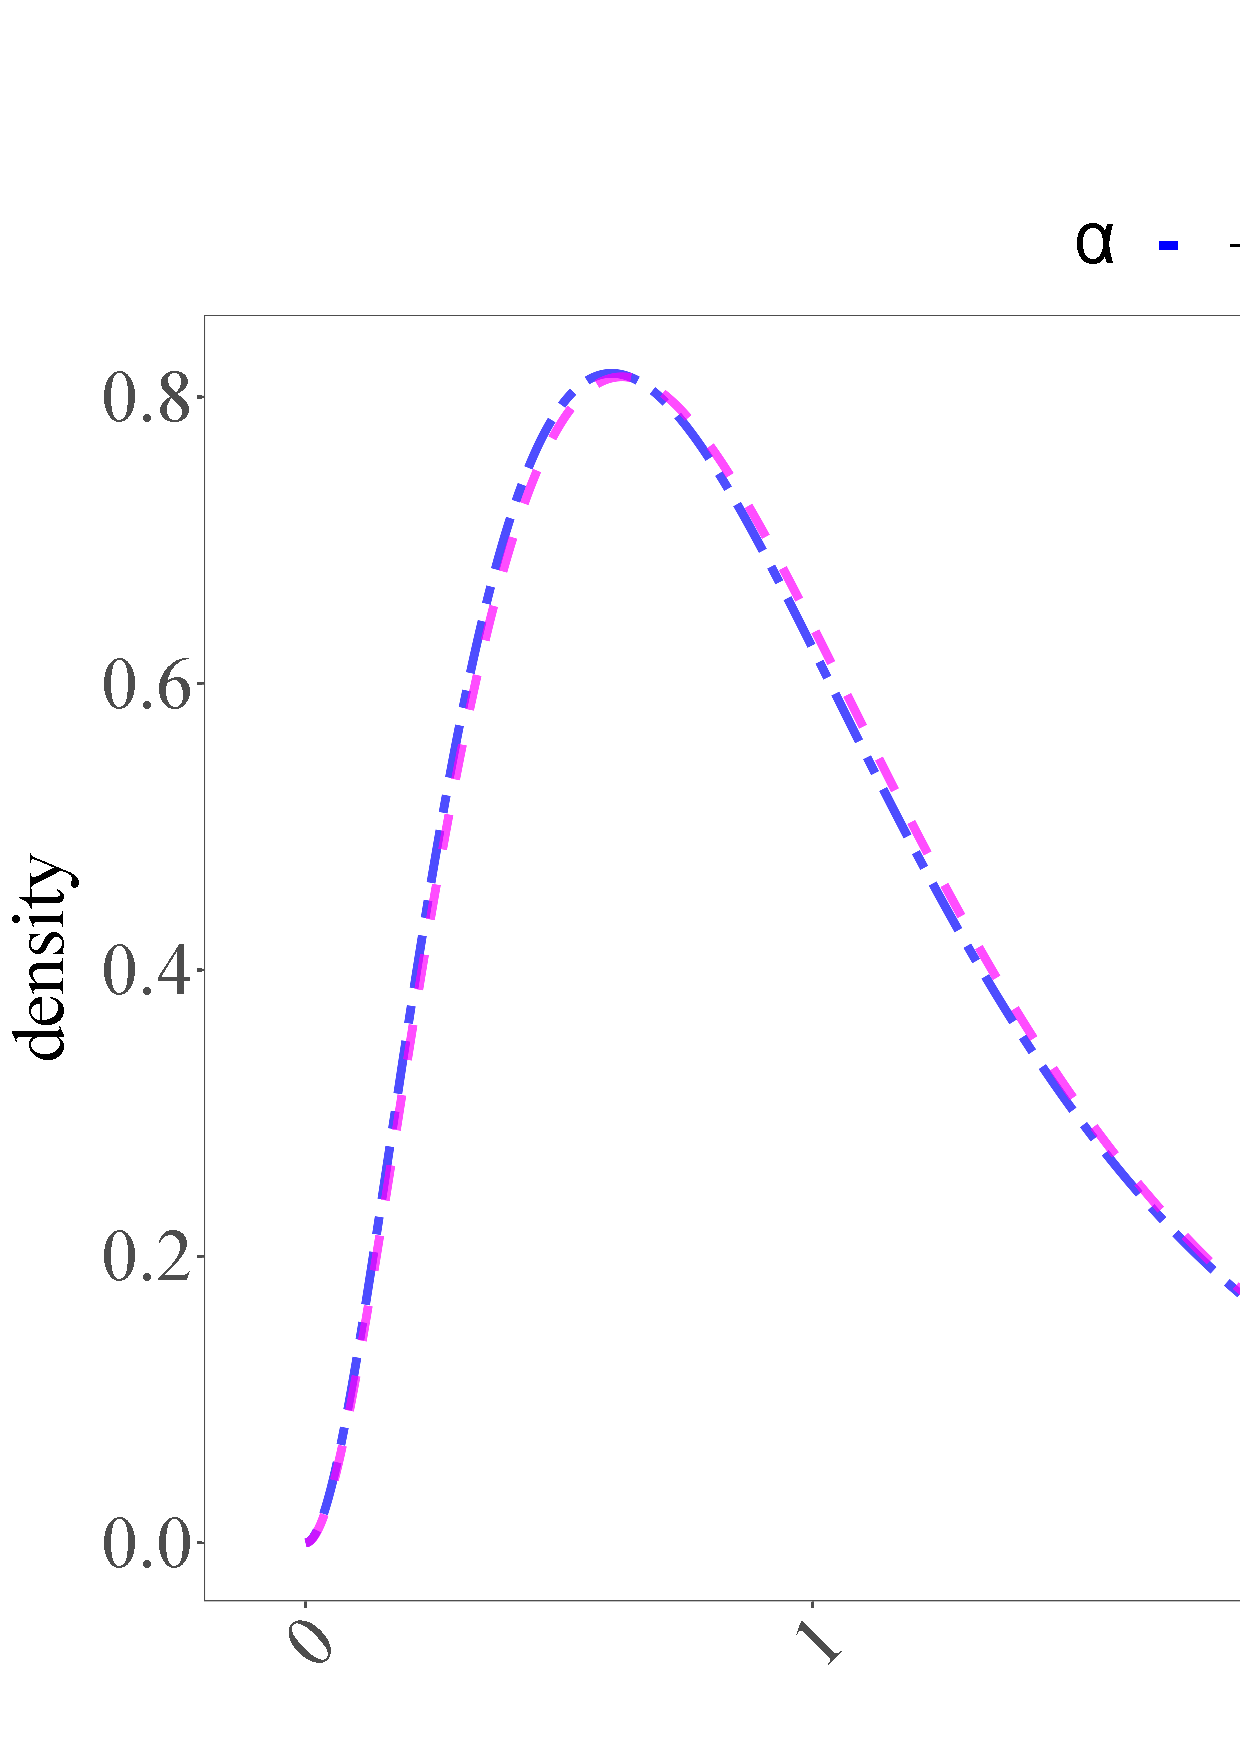
\includegraphics[width=.48\linewidth]{../../Figures/Tesis/Capitulo4/DensidadGI0L3.pdf}}
	\subfigure[Escala semilogarítmica\label{EscalaSemiLog}]{\includegraphics[width=.48\linewidth]{../../Figures/Tesis/Capitulo4/DensGI0_L3_Semilog.pdf}}
	\caption{\label{DensidadGI0L03}Densidad $\mathcal{G}_I^0$ para $L=3$ y $\alpha=-1.5, \, -5, \, -8$.}
\end{figure} 

En la figura~\ref{DensidadGI0TodoL} se muestra el gráfico de la densidad $\mathcal{G}_I^0$ para $L=1, \, 3, \, 8$ y $\alpha= -5$. Se puede obervar el efecto multilook, a medida que el número de looks aumenta, las colas son menos pesadas.

\begin{figure}[hbt]
	\centering    
	\includegraphics[width=.5\linewidth]{../../Figures/Tesis/Capitulo4/DensGI0_TodoL_Semilog.pdf}
	\caption{\label{DensidadGI0TodoL}Densidad $\mathcal{G}_I^0$ para $L=1, \, 3, \, 8$ y $\alpha= -5$.}
\end{figure} 

Bajo este modelo se pueden caracterizar regiones con diferentes grado de textura a través de los parámetros de la distribución $\mathcal{G}_I^{0}$. Para valores de $\alpha$ cercanos a cero (típicamente en el intervalo $(-3,0)$), la zona de la imagen corresponde a una región muy texturada, como es el caso de las zonas urbanas en las imágenes SAR. A medida que el valor del parámetro $\alpha$ disminuye, corresponde a zonas con cada vez menos textura, como son las regiones de forestación (usualmente $(-6,-3]$) y pastura (en $(-\infty,-6)$). Por otro lado, el parámetro $\gamma$ (llamado parámetro de escala) posee una interpretación en términos del brillo. Cuanto mayor es su valor, mayor intensidad posee la imagen en esa región. Por estas razones, la estimación precisa de los parámetros es de suma importancia en el análisis de imágenes con ruido speckle. 



%%%%%%%%%%%%%%%%%%%%%%%%%%%%%%%%%%%%%%%%%%%%%%%%%%%%%%%%%%%%
\section{Resultados Teóricos}
\label{ResultadosTeoricosGI0}

En esta sección se darán nuevos resultados teóricos presentados en \citet{gambini2015}, que muestran que la distribución $\mathcal{G}_I^0$ es una distribución de colas pesadas. Esto explica en parte los problemas que se enfrentan al buscar estimadores de los parámetros de esta distribución.  También se presentan nuevos resultados sobre el comportamiento asintótico de la distribución $\mathcal{G}_I^0$ respectos de sus parámetros, que se necesitarán para demostrar la consistencia del estimador del parámetro de textura $\alpha$ propuesto en esta tesis.

\subsection{La ley $\mathcal{G}_I^0$ es una distribución de colas pesadas}
\label{colas}
Siguiendo a \citet{Gre,Jorgensen,Rojo} daremos las siguientes definiciones.

\begin{definition} \label{Def:lenta}
	La función $\ell\colon\mathbb R \to\mathbb R$ es de variación lenta en el infinito si para todo $t>0$ vale que
	$$
	\lim_{x\to+\infty}\dfrac{\ell (tx)}{\ell(x)}=1.
	$$
\end{definition}

\begin{definition} 
	Una función de densidad de probabilidad $f(x)$ tiene colas pesadas si para algún $\eta >0$ vale que
	$$
	f(x)=\ell(x)  x^{-\eta},
	$$
	donde $\ell$ es una función de variación lenta en el infinito y $\eta$ es el índice de la cola.
\end{definition}
Cuanto menor es el índice de la cola, más propensa es la distribución a producir observaciones extremas.

\begin{proposition}
	La distribución $\mathcal G_{I}^0$ tiene colas pesadas con índice de la cola igual a $1-\alpha$.
\end{proposition}
\begin{proof}
	Si definimos $\ell(x)=f_{\mathcal G_I^0}(x) x^{-\alpha+1}$ tenemos que
	\begin{align*}
	\lim_{x\to+\infty}\frac{\ell(t x)}{\ell(x)}&=\lim_{x\to+\infty}\frac{(tx)^{L-1} \, (Ltx+\gamma)^{\alpha-L} \, (tx)^{1-\alpha}}{x^{L-1} \, (Lx+\gamma)^{\alpha-L} \, x^{1-\alpha}}\\
	&=\lim_{x\to+\infty}t^{L-\alpha}\left(\frac{Lx+\gamma}{L tx+\gamma}\right)^{L-\alpha}=1.
	\end{align*}
	Esto vale para todo $t>0$, por lo tanto $\ell$ es de variación lenta en el infinito.
\end{proof}
Se puede ver que el índice de la cola es una función decreciente de $\alpha$, entonces la distribución $\mathcal G_I^0$ es más propensa a producir valores extremos cuando el parámetro de textura es más grande. Esto va de acuerdo a lo mostrado en la figura~\ref{DensidadGI0L03}.

\subsection{Comportamiento asintótico de la distribución $\mathcal{G}_I^0$}
Estos resultados se probarán considerando el caso $E(Z)=1$ que nos da una relación entre los parámetros de la distribución $\mathcal{G}_I^0$: $\gamma^*=-\alpha-1$. Como el parámetro $\gamma$ es considerado un parámetro de escala, con esta relación logramos que los resultados para diferentes áreas resulten comparables.
 
En este caso se puede escribir a $f_{\mathcal{G}_I^0}\pa{z}$ en términos de $\gamma$. De esta forma, la función de distribución del modelo $\mathcal{G}_I^0$ bajo esta condición queda:
\begin{align}
\label{fenfunciondegamma}
f_{\gamma}\pa{z}=\frac{\Gamma\pa{L+\gamma+1}}{\Gamma\pa{\gamma+1}\Gamma\pa{L}}
\pa{\frac{L}{\gamma}}^L \frac{z^{L-1}}{\pa{1+\frac{Lz}{\gamma}}^{L+\gamma+1}}.
%f_{\mathcal{G}_I^0}\pa{z} = \frac{\Gamma\pa{L+\gamma+1}}{\Gamma\pa{\gamma+1}\Gamma\pa{L}}
%L^{-1-\gamma} z^{-2-\gamma} \gamma^{\gamma +1} \pa{1+\frac{\gamma}{L z}}^{-\gamma -L-1}.
\end{align}

Vamos a utilizar esta forma de escribir a $f_{\mathcal{G}_I^0}\pa{z}$ en las proposiciones~\ref{conv1} y ~\ref{conv2}.

\begin{proposition}
	\label{conv1}
	Para todo intervalo compacto $[z_{1},z_{2}]\subset\pa{0,\infty}$, $f_{\mathcal{G}_I^0}\pa{z}$ converge
	uniformemente a $\Gamma(\text{L,L})$ en $[z_{1},z_{2}]$ si $\alpha\to -\infty$,
	donde $\Gamma(\text{L,L})$ es la función de densidad del modelo $\Gamma$ con parámetros $\pa{\text{L,L}}$.
\end{proposition}

\begin{dem}
Si consideramos $f_{\mathcal{G}_I^0}\pa{z}$ escrita como en~\eqref{fenfunciondegamma} estudiar la convergencia de $f_{\mathcal{G}_I^0}\pa{z}$ cuando $\alpha\to -\infty$ es equivalente a estudiar el $\lim\limits_{\gamma\to+\infty} f_{\gamma}\pa{z}$. 
		
Si llamamos:
	\begin{align*}
		a\pa{\gamma} &= \frac{\Gamma\pa{\gamma+1}\e^{\gamma}}{\sqrt{2\pi}\gamma^{\gamma+1/2}},\\
%		b\pa{L,\gamma,z} &=L\gamma^{L-1}\pa{\frac{\frac{Lz}{\gamma}}{1+\frac{Lz}{\gamma}}}^{L-1} \text{ y }\\
%		c\pa{L,\gamma,z} &= \pa{1+\frac{Lz}{\gamma}}^{-2-\gamma},
	\end{align*}
entonces 
\begin{align}
\label{GIOfunciongamma}
f_{\gamma}\pa{z} = \frac{a\pa{L+\gamma}}{a\pa{\gamma}\Gamma\pa{L}}\e^{-L}\pa{1+\frac{L}{\gamma}}^{L+\gamma+1/2} \dfrac{L^L z^{L-1}}{\left(1+\dfrac{L z}{\gamma}\right)^{L+\gamma +1}}.
\end{align}

%\begin{align*}
%	\lim_{\gamma\to+\infty}\frac{\Gamma\pa{L+\gamma+1}}{\Gamma\pa{\gamma+1}\Gamma\pa{L}}
%	\frac{L}{\gamma}\pa{\frac{\frac{Lz}{\gamma}}{1+\frac{Lz}{\gamma}}}^{L-1}
%	\pa{1+\frac{Lz}{\gamma}}^{-2-\gamma},
%\end{align*}

De la fórmula de Stirling se obtiene que
	\begin{align*}
	% \lim_{\gamma\to+\infty} a\pa{L,\gamma} = 
	% \al \lim_{\gamma\to+\infty}\frac{\Gamma\pa{L+\gamma+1}\e^{L+\gamma}}{\sqrt{2\pi}\pa{L+\gamma}^{L+\gamma+1/2}} = 1,\\
	\lim_{\gamma\to+\infty} a\pa{\gamma} = 
	\al \lim_{\gamma\to+\infty}\frac{\Gamma\pa{\gamma+1}\e^{\gamma}}{\sqrt{2\pi}\gamma^{\gamma+1/2}} = 1,
	\end{align*}
entonces
	\begin{align*}
	1=\lim_{\gamma\to+\infty} \frac{a\pa{L+\gamma}}{a\pa{\gamma}} = 
	\al \lim_{\gamma\to+\infty}\frac{\Gamma\pa{L+\gamma+1}}{\Gamma\pa{\gamma+1}}
	\e^{L}\gamma^{-L}\pa{1+\frac{L}{\gamma}}^{-L-\gamma-1/2}.
	\end{align*}

	Por otro lado, se verifica que
	\begin{align}
	\label{b}
	\lim_{\gamma\to+\infty} \left(1+\dfrac{L}{\gamma}\right)^{L+\gamma +1/2}=e^L,\\
	\label{c}
	\lim_{\gamma\to+\infty} \left(1+\dfrac{L z}{\gamma}\right)^{-(L+\gamma +1)}=e^{-L z} ,
%	\label{b}
%	\nonumber \lim_{\gamma\to+\infty} b\pa{L,\gamma,z} =
%	\al \lim_{\gamma\to+\infty}L\gamma^{L-1}\pa{\frac{\frac{Lz}{\gamma}}{1+\frac{Lz}{\gamma}}}^{L-1} \\
%	= \al \lim_{\gamma\to+\infty} \frac{L^{L} z^{L-1}}{\pa{1+\frac{Lz}{\gamma}}^{L-1}} = L^{L} z^{L-1},\\
%	\lim_{\gamma\to+\infty} c\pa{L,\gamma,z} = \al \lim_{\gamma\to+\infty}\pa{1+\frac{Lz}{\gamma}}^{-2-\gamma} = \e^{-Lz},
%	\label{c}
	\end{align}
	donde la convergencia en~\eqref{c} es uniforme en $[z_{1},z_{2}]$.
	
	Entonces se obtiene que $\lim\limits_{\gamma\to+\infty}f_{\gamma}\pa{z} = L^{L}/\Gamma\pa{L}\,\e^{-Lz}z^{L-1}$ uniformemente en $[z_{1},z_{2}]$, donde $f_{\gamma}\pa{z}$ es la función de densidad dada en~\eqref{GIOfunciongamma}.
\end{dem}

La figura~\ref{ConvInfinito} ilustra la convergencia uniforme de $f_{\mathcal{G}_I^0}\pa{z}$ a $\Gamma(3,3)$, cuando $\alpha \to -\infty$ y $L=3$. 
El área gris es una banda de ancho $\epsilon=0.1$ alrededor de la función de densidad $\Gamma(3,3)$ (línea sólida). 
La línea punteada y la línea discontinua representan $f_{\mathcal{G}_I^0}\pa{z}$ para $\alpha=-20$ y $\alpha=-8$ respectivamente. 
Se puede ver que, cuando $\alpha$ disminuye, $f_{\mathcal{G}_I^0}\pa{z}$ cae dentro del área gris. 
Mas aún, para este valor de $\epsilon$, $f_{\mathcal{G}_I^0}(-20)$ ya cae dentro de esa banda.


\begin{figure}[hbt]
\begin{center}
	\includegraphics[scale=0.8]{../../Figures/Tesis/Capitulo4/ConvUniformeMenosInfinito2.pdf}
	\caption{\label{ConvInfinito}\small{Convergencia uniforme de $f_{\mathcal{G}_I^0}\pa{z}$ a $\Gamma(3,3)$ cuando $\gamma=\gamma^*$, $\alpha \to -\infty$, $L=3$ y $\epsilon=0.1$.}}
\end{center}
\end{figure} 


\begin{proposition}
	\label{conv2}
	Para todo intervalo compacto $[z_{1},z_{2}]\subset\pa{0,\infty}$, $f_{\mathcal{G}_I^0}\pa{z}$ converge
	uniformemente a $0$ en $[z_{1},z_{2}]$, si $\alpha\to -1^{-}$.
\end{proposition}
\begin{dem}
	En forma equivalente a la proposición~\ref{conv1} y usando la relación entre $\alpha$ y $\gamma$, estudiar la convergencia de $f_{\mathcal{G}_I^0}\pa{z}$ cuando $\alpha\to -1^{-}$ es equivalente a estudiar ese límite cuando ${\gamma\to 0^{+}}$.
	De~\eqref{fenfunciondegamma}:
	\begin{align*}
	f_{\gamma}\pa{z} = &\frac{\Gamma\pa{L+\gamma+1}}{\Gamma\pa{\gamma+1}\Gamma\pa{L}}
	L^{L} \frac{z^{L-1}}{(\gamma+Lz)^{L+\gamma+1}} \gamma^{\gamma +1}  \\
	\leq& \frac{\Gamma\pa{L+\gamma+1}}{\Gamma\pa{\gamma+1}\Gamma\pa{L}}
	L^{L} \frac{z_2^{L-1}}{(\gamma+Lz_1)^{L+\gamma+1}} \gamma^{\gamma +1} .
	\end{align*}
	Dado que $\Gamma$ es una función continua, para $z \in [z_{1},z_{2}]$, $\lim\limits_{\gamma\to0^+} f_{\gamma}\pa{z}=0$ uniformemente en $z$, con lo que se obtiene el resultado.
\end{dem}

La figura~\ref{ConvEnCero} ilustra la convergencia uniforme de $f_{\mathcal{G}_I^0}\pa{z}$ cuando $\alpha \to -1$ y $L=3$. La banda gris es de ancho $\epsilon=0.2$ alrededor del eje $z$. 
Se graficaron tres diferentes densidades con líneas punteada, discontinua y sólida, las cuales representan $f_{\mathcal{G}_I^0}\pa{z}$ para $\alpha=-1.01, \ -1.2$ y $-1.5$ respectivamente. 
Se puede ver que cuando el valor de $\alpha$ se acerca a $-1$, $f_{\mathcal{G}_I^0}\pa{z}$ se aplana a $0$, excepto para $z=0$. 
Para  $\epsilon=0.2$ y cualquier intervalo $[z_1,z_2]$ considerado, $f_{\mathcal{G}_I^0}\pa{z}$ cae dentro de esta banda para $\alpha$ suficientemente cercano a $-1$. 
Por ejemplo, para el intervalo $[1.5,2]$ y para este valor de $\epsilon$, $f_{\mathcal{G}_I^0}\pa{z}$ entra en la banda gris desde $\alpha=-1.5$. 
Si el intervalo es $[0.5,1]$ esto sucede a partir de $\alpha=-1.01$.



\begin{figure}[hbt]
	\centering    
	\includegraphics[width=0.8\linewidth]{../../Figures/Tesis/Capitulo4/ConvUnifEnCero.pdf}
	\caption{\label{ConvEnCero}Convergencia uniforme de $f_{\mathcal{G}_I^0}\pa{z}$ a $0$ cuando $\gamma=\gamma^*$, $\alpha \to -1$, $L=3$ y $\epsilon=0.2$.}
\end{figure}

\section{Conclusiones}

En este capítulo presentamos varias distribuciones que se utilizan para modelar datos provenientes de imágenes SAR:
\begin{itemize}
	\item Los llamados modelos empíricos que son distribuciones que se propopnen para ajustar datos SAR, como la distribución Lognormal, Weibull entre otras.
	\item El modelo multiplicativo, que establece que el retorno $Z$ se modela como el producto de dos variables aleatorias: $X$ para la retrodispersión e $Y$ para el ruido speckle.
\end{itemize} 

Mostramos un abordaje donde se explica la naturaleza multiplicativa del ruido speckle. A partir de esto se propuso modelar al ruido speckle $Y$ con una distribución $\Gamma(L,L)$ en el caso de datos en formato intensidad y monopolarizados, donde $L$ es el número de looks. En cuanto a la retrodispersión $X$ se propone modelarla con una distribución gaussiana inversa generalizada $N^{-1}(\alpha,\gamma,\lambda)$. Para valores particulares de los parámetros de la distribución $N^{-1}(\alpha,\gamma,\lambda)$, se obtienen las distribuciones $\Gamma(\alpha,\lambda)$, $\Gamma^{-1}(\alpha,\gamma)$ e $IG(\gamma, \lambda)$. Bajo el modelo multiplicativo estas distribuciones para la retrodispersión dan origen a las distribuciones $\mathcal{K}$, $\mathcal{G}_I^0$ y $\mathcal{G}^H$ para el retorno $Z$, respectivamente. 

En esta tesis utilizamos el modelo $\mathcal{G}_I^0$ para datos de intensidad. Presentamos la función de distribución y demostramos que es una distribución que tiene colas pesadas.

Asimismo demostramos resultado sobre la convergencia uniforme de la distribución $\mathcal{G}_I^0$ cuando el parámetro de textura se acerca a $-1$ y a $-\infty$ para el caso donde $E(Z)=1$.




%\begin{proposition}
%	\label{pr: falpha>0}
%	Para todo $\alpha\in I$, existe $U$ un entorno compacto de $\alpha$ tal que
%	$\inf\limits_{\alpha'\in I-U}d_{T}\pa{f_{\alpha'};f_{\alpha}}>0$.
%\end{proposition}
%\begin{dem}
%	Siendo que $f_{\alpha}\ne f_{\Gamma,L,L}$, existe $[z_{1},z_{2}]\subset\pa{0,\infty}$, tal que
%	\begin{align*}
%	\int_{z_{1}}^{z_{2}}\frac{\pa{f_{\alpha}\pa{z}-f_{\Gamma,L,L}\pa{z}}^{2}}
%	{f_{\alpha}\pa{z}+f_{\Gamma,L,L}\pa{z}}dz >0,
%	\end{align*}
%	entonces
%	\begin{align*}
%	\liminf_{\alpha'\to-\infty} d_{T}\pa{f_{\alpha'};f_{\alpha}} 
%	\ge \al \liminf_{\alpha'\to-\infty}\int_{z_{1}}^{z_{2}}\frac{\pa{f_{\alpha}\pa{z}-f_{\alpha'}\pa{z}}^{2}}
%	{f_{\alpha}\pa{z}+f_{\alpha'}\pa{z}}dz \\
%	= \al \int_{z_{1}}^{z_{2}}\frac{\pa{f_{\alpha}\pa{z}-f_{\Gamma,L,L}\pa{z}}^{2}}
%	{f_{\alpha}\pa{z}+f_{\Gamma,L,L}\pa{z}}dz >0.
%	\end{align*}
%	De la misma forma
%	\begin{align*}
%	\liminf_{\alpha'\to-1^{-}} d_{T}\pa{f_{\alpha'};f_{\alpha}} 
%	\ge \al \liminf_{\alpha'\to-1^{-}}\int_{z_{1}}^{z_{2}}\frac{\pa{f_{\alpha}\pa{z}-f_{\alpha'}\pa{z}}^{2}}
%	{f_{\alpha}\pa{z}+f_{\alpha'}\pa{z}}dz \\
%	= \al \int_{z_{1}}^{z_{2}}f_{\alpha}\pa{z}dz >0,
%	\end{align*}
%	lo que prueba la proposición.
%\end{dem}
%\begin{corollary}
%	Si $\set{\alpha_{k}}_{k\in\N}$ una sucesión de $I$ tal que $d_{T}\pa{f_{\alpha_{k}};f_{\alpha}}\to 0$,
%	entonces $\alpha_{k}\to\alpha$.
%\end{corollary}
%\begin{dem}
%	Es consecuencia de las proposiciones \ref{pr: convergencia} y \ref{pr: falpha>0}.
%\end{dem}
%% Los cap'itulos inician con \chapter{T'itulo}, estos aparecen numerados y
%% se incluyen en el 'indice general.
%%
%% Recuerda que aqu'i ya puedes escribir acentos como: 'a, 'e, 'i, etc.
%% La letra n con tilde es: 'n.

\chapter{Metodología}
\label{metodologia}

Es sabido que tener información sobre la función de densidad o distribución de una variable aleatoria permite tener una completa descripción de la misma. Por este motivo es un problema fundamental de la Estadística obtener, a partir de la información proporcionada por una muestra,  buenas estimaciones de las funciones de densidad de una variable o vector aleatorio. 

En este sentido existen dos enfoques para abordar este problema. 

\begin{itemize}
	\item Un enfoque paramétrico: donde se considera que la función de densidad teórica pertenece a una familia de funciones de densidad $f_X(\theta)$ conocida, indexada por el vector de parámetros $\theta$. Bajo esta suposición estimar la función de densidad teórica se reduce a estimar el valor de los parámetros del modelo a partir de la información proporcionada por la muestra. Los métodos clásicos de estimación paramétrica son: Método de los Momentos y Método de Máxima Verosimilitud. En los últimos años el Método de LogCumulantes, que se basa en la transformada de Mellin, ha ganado interés por su buena performance.
	\item Un enfoque no paramétrico: donde no se hace ninguna suposición inicial sobre la familia de densidades a las que pertenece la función de densidad teórica, sino que trata de estimarla teniendo como única información los datos muestrales, imponiendo  solamente las condiciones necesarias para que dicha estimación sea una función de densidad.
\end{itemize}

El principal aporte de esta tesis es la propuesta de un nuevo método de estimación para los parámetros del modelo $\mathcal G_I^0$ con buenas propiedades que serán estudiadas a través del sesgo, del error cuadrático medio y de su capacidad para resistir presencia de datos atípicos, aún en el caso de muestras de pequeño y moderado tamaño. Este estimador surge de la minimización de distancias estocásticas entre la función de densidad teórica y una estimación no paramétrica de la función densidad subyacente utilizando núcleos asimétricos. 

En este capítulo describimos dos metodologías de estimación de la función de densidad: paramétrica y no paramétrica. Presentamos los estimadores de momento, de máxima verosimilitud y logcumulante del parámetro de textura de la distribución $\mathcal{G}_I^0$, que son los estimadores que utilizaremos para evaluar la performance del propuesto en esta tesis. También presentamos los conceptos de estimación no paramétrica de la función de densidad, núcleos asimétricos, distancias estocásticas y estimadores de mínima distancia estocástica porque son el corazón del estimador planteado.  Asimismo hacemos una discusión de diferentes distancias estocásticas estudiadas y diferentes núcleos utilizados para estimar la función de densidad subyacente. Finalmente nuestra propuesta para estimar el parámetro de textura del modelo $\mathcal{G}_I^0$ que es el argumento que minimiza una distancia estocástica entre la función de densidad teórica del modelo teórico y una estimación no paramétrica de la función de densidad subyacente. 


\section{Estimación Paramétrica}
\label{EstimacionParamétrica}

Esta metodología de estimación propone, a partir del conocimiento de la familia de densidades a la que pertenece la función de densidad teórica, estimar los parámetros que caracterizan dicha función de densidad a partir de datos muestrales. A continuación presentaremos métodos clásicos de estimación paramétrica.

\subsection{Método de los Momentos}
El Método de los Momentos (MOM) fue introducido por Karl Pearson en el año 1894 y se basa en la idea intuitiva de pensar que, si los datos muestrales provienen de una determinada función de densidad entonces los momentos muestrales deberían dar buenas estimaciones de los correspondientes momentos poblacionales. 

\begin{definition}
Si $X_1, \ldots, X_n$ es una muestra de variables aleatorias independientes e idénticamente distribuidas con función de densidad $f_{X;\theta}$, donde $\theta \in \mathbb{R}$ es el parámetro a estimar, y $g(x)$ una función de $\mathbb{R}$ en $\mathbb{R}$, el Método de los Momentos propone como estimador $\hat{\theta}_{mom}$ de $\theta$ aquel valor del parámetro que es solución de la ecuación  $\dfrac{1}{n} \sum_{i=1}^n g(X_i)=E_{\theta}(g(X_i)).$  
Si en cambio $X_i \sim f_{X;\theta}$ con $\theta \in \Theta \subset \mathbb{R}^k$, entonces $\hat{\theta}_{mom}$ será el valor $\theta$ que verifica el sistema de ecuaciones $\dfrac{1}{n} \sum_{i=1}^n g_s(X_i)=E_{\theta}(g_s(X_i))$ donde $s=1, \ldots k$ y $g_s(x)$ son $k$ funciones de $\mathbb{R}$ en $\mathbb{R}$.
\end{definition}


Obsevemos que si $g_s(x)=x^s$ la definición es consistente con la idea intuitiva mencionada anteriormente.
%Entonces, si $g(x)=x$ y el correspondiente momento muestral es $m_k=\dfrac{\sum_{i=1}^n X_i^k}{n}$. Entonces, si $X_1, \ldots X_n$ es una muestra de variables aleatorias independientes e idénticamente distribuidas 
%
%Recordemos que el $k$-ésimo momento muestral de una variable aleatoria $X$, tomado alrededor del origen, es $M_k=E(X^k)$.

El estimador por Momentos Fracionales ha sido estudiado en los últimos tiempos~\cite{Frery97,GambiniSC08,Khan2013}. En esta tesis se utilizarán los momentos de orden $1$ y de orden $\frac{1}{2}$ porque mostraron una mejor performance a la hora de estimar los parámetros de la distribución $\mathcal G_I^0$ respecto de los momentos de orden $1$ y de orden $2$.

Las ecuaciones de momento de orden $1$ y de orden $\frac{1}{2}$ para estimar los parámetros de la distribución $\mathcal G_I^0$ son:

\begin{align}
\label{momento1medio}
\nonumber \overline{X}=&\dfrac{\gamma}{-\alpha - 1}, \\
\nonumber \\ 
\dfrac{\sum_{i=1}^n X_i^{1/2}}{n}=&\dfrac{\gamma^{1/2}}{L^{1/2}}\dfrac{\Gamma(-\alpha - 1/2)}{\Gamma(-\alpha)}\dfrac{\Gamma(L+ 1/2)}{\Gamma(L)}.
\end{align}


\subsection{Método de Máxima Verosimilitud}

\textcolor{blue}{
 El Método de Máxima Verosimilitud fue popularizado por R. Fisher entre 1912 y 1922. Sin embargo este método había sido utilizado antes por Gauss, Laplace entre otros investigadores. La idea del método consiste en, dada una muestra, estimar los parámetros de la distribución que maximice la probabilidad de que haya salido esa muestra. Esto requiere mirar a la función de densidad conjunta como función de los parámetros, habiendo salido la muestra. A esta función se llama fución de verosimilitud.
\begin{definition}
Si $X_1, \ldots, X_n$ es una muestra de variables aleatorias independientes e idénticamente distribuidas con función de densidad $f_{X;\theta}$  con $\theta \in \Theta \subset \mathbb{R}^k$, diremos que $\widehat{\theta}_{\text{MV}}$ es el estimador de máxima verosimilitud de $\theta$ si verifica que 
\begin{align}
\widehat{\theta}_{{\text{\tiny{\text{MV}}}}}=\arg\max_{\vec{\theta \in \Theta}} L(\theta \mid \vec{X}=\vec{x}),
\end{align}
siendo $L(\theta \mid \vec{X}=\vec{x})$ la función de verosimilitud, que es la función de densidad conjunta del vector aleatorio $\vec{X}$ mirada como función del vector de parámetros $\theta$, sabiendo que salió la muestra $\vec{x}$.
\end{definition}
Este estimador tiene muy buenas propiedades asintóticas, además de ser consistente es asintóticamente normal y eficiente bajo condiciones generales.
}

El parámetro $\gamma$ en la distribución $\mathcal{G}_I^0$  es proporcional al brillo y es un parámetro de escala. Con el fin de reducir nuestro análisis a un solo parámetro, y con el propósito de hacer los resultados comparables, basamos nuestro análisis en la condición $E(Z)=1$ que vincula la textura con el brillo. Esta condición nos da una relación entre $\gamma$ y $\alpha$ que es la siguiente:
\begin{align}
\label{gama*}
\gamma=-\alpha-1. 
\end{align}
A este valor de $\gamma$ lo llamaremos $\gamma^*$.

Entonces, si $Z_1,\ldots Z_n$ una muestra de variables aleatorias independientes e idénticamente distribuidas donde $Z_i \sim f_{\mathcal G_I^0(\alpha,\gamma)}(z)$,  el logaritmo de la función de verosimilitud bajo la condición~\eqref{gama*} es:

\textcolor{blue}{
\begin{align}
\nonumber \log (L(\alpha) \mid \vec{Z}=\vec{z})&=n(L \log L+\log \Gamma(L-\alpha)-\log \Gamma(-\alpha) -\alpha \log(-\alpha-1))\\
& + (L-1) \sum_{i=1}^n \log(z_i)-(L-\alpha) \sum_{i=1}^n\log(-\alpha-1+z_i L).
\end{align}
}

Por lo tanto, el estimador de máxima verosimilitud (ML) del parámetro de textura es:
\begin{align}
\widehat{\alpha}_{{\text{\tiny{MV}}}}=\arg\max_{\alpha} \log(L(\alpha)/\vec{Z}=\vec{z}).
\end{align}

Algunos autores evaluaron la performance para el estimador de máxima verosimilitud del parámetro de textura del modelo  $\mathcal G_I^0$. Vasconcellos et al.~\cite{VasconcellosFrerySilva:CompStat} cuantificaron el sesgo de este estimador y propusieron una corrección de segundo orden de acuerdo a~\cite{cox1968}. Cribari-Neto et al.~\cite{CribariFrerySilva:CSDA} desarrollaron una corrección del sesgo de $\widehat{\alpha}_{\text{{\text{\tiny{ML}}}}}$ del modelo $\mathcal G^0$ para datos de amplitud usando técnicas de remuestreo a expensas de un alto costo computacional.

En la figura~\ref{MV} se muestra el gráfico del logaritmo de la función de verosimilitud en función de $\alpha$, para distintos tamaños de muestra $n$ y para dos valores del parámetro de textura: $\alpha=-1.5$ y $\alpha=-5$ para el caso de $L=3$. Se puede observar que, para zonas extremadamente texturadas la función de verosimilitud muestra claramente un máximo. Sin embargo, para el caso de zonas texturadas esta función es bastante plana, incluso podría ser monótona dependiendo de la muestra. Esto puede originar problemas numéricos al momento de encontrar el máximo.  

\begin{figure}[hbt]
	\centering    
	\subfigure[$\alpha=-1.5$]{\includegraphics[width=.45\linewidth]{../../Figures/Tesis/Capitulo5/Verosimilitud1punto5_2.pdf}} \qquad
	\subfigure[$\alpha=-5$]{\includegraphics[width=.45\linewidth]{../../Figures/Tesis/Capitulo5/Verosimilitud-5_2.pdf}}
	\caption{\label{MV} Función de verosimilitud para $L=3$}
\end{figure}

También se podría encontrar $\widehat{\alpha}_{{\text{\tiny{MV}}}}$ como la solución de la siguiente ecuación no lineal.

\begin{align}
\label{rootML}
\Psi^0(-\widehat{\alpha}_{{\text{\tiny{MV}}}})-\Psi^0(L-\widehat{\alpha}_{{\text{\tiny{MV}}}})-\log(-1-\widehat{\alpha}_{{\text{\tiny{MV}}}})+{} \nonumber\\
\frac{\widehat{\alpha}_{{\text{\tiny{MV}}}}}{-1-\widehat{\alpha}_{{\text{\tiny{MV}}}}}+
\frac{1}{n}\sum_{i=1}^n{\log(-1-\widehat{\alpha}_{{\text{\tiny{MV}}}}+Lz_i)}-{}
\nonumber
\\ \frac{\widehat{\alpha}_{{\text{\tiny{MV}}}}-L}{n}\sum_{i=1}^n \frac1{-1-\widehat{\alpha}_{{\text{\tiny{MV}}}}+Lz_i}= 0, 
\end{align}
donde $\Psi^0(\cdot)$ es la función digamma. Este sistema no tiene una solución analítica cerrada, por lo tanto es necesario la utilización de rutinas numéricas para encontrar dicha solución que puede incluso no existir.

\subsection{Log Momentos y Log Cumulantes}

Es conocida la relación que existe entre los momentos y la función característica de una variable aleatoria con la transformada de Fourier de su función de densidad. 

\begin{definition}
Si $X$ es una variable aleatoria continua con función de densidad $f_X(x)$, la función característica $\phi_X: \mathbb{R} \rightarrow \mathbb{C}$ se define como 
\begin{align}
\phi_X(t)=E(e^{itX})=\int_{-\infty}^{\infty} e^{itx} f_X(x) dx = \mathcal{F}\{f_X\}(t),
\label{fi}
\end{align}
siendo $\mathcal{F}\{f_X\}$ la transformada de Fourier de $f_X$.
\end{definition}

Cuando los momentos de orden $n$ de una variable aleatoria existen, es decir, cuando $E(X^k)< \infty$, se puede apelar a la relación~\eqref{fi} para calcular dichos momentos. Entonces

\begin{align}
\phi_X^{(k)}(0)=i^k E(X^k),
\label{fi}
\end{align}
con $\phi_X^{(k)}$ la derivada de orden $k$ de $\phi_X$ evaluada en $t=0$. Luego, los momentos de orden $k$ se pueden definir como 

\begin{align}
\label{MomentosPrimerTipo}
m_k=E(X^k)=i^{-k} \phi_X^{(k)}(t)\big\arrowvert _{t=0}\cdot
\end{align}

Si llamamos $\psi_X=\log(\phi_X)$, los cumulantes de orden $k$ se definen como 

\begin{align}
\label{CumulantePrimerTipo}
\kappa_k=i^{-k} \psi_X^{(k)}\big\arrowvert _{t=0}\cdot
\end{align}

Nicolas et al.~\cite{nicolas2002} proponen utilizar la transformada de Mellin en lugar de la transformada de Fourier en~\eqref{fi}, para el caso donde la función de densidad $f_X$ de la variable aleatoria $X$ tiene soporte positivo. De esta manera surgen nuevas características para la variable aleatoria que son los Log Momentos (MomL) y los Log Cumulantes (MomLC). Los autores proponen llamar a esta metodología Estadísticas de Segundo Tipo. Entonces, análogamente a la metodología descripta en~\ref{fi}, definen:

\begin{itemize}
\item Primer función característica de segundo tipo.
	\begin{align}
	\Phi_X(s)=\int_{0}^{\infty} x^{s-1} f_X(x) dx = \mathcal{M}\{f_X\}(s)\cdot
	\label{PrimerFuncionCaract}
	\end{align}
\item Momentos de segundo tipo.
	\begin{align}
	\label{MomentoSegundoTipo}
	\tilde{m}_k=\Phi_X^{(k)}(s) \big\arrowvert _{s=1}\cdot
	\end{align}


	Una propiedad interesante que cumplen las derivadas de orden $k$ de la transformada de Mellin de una función $h(x)$ es $\mathcal{M}\{\ln(x)^k h(x)\}(s)=\mathcal{M}^{(k)}\{h(x)\}(s)$. Entonces, aplicando esta propiedad a~\eqref{PrimerFuncionCaract} y~\eqref{MomentoSegundoTipo}, y considerando $h=f_X$ se obtiene:

	\begin{align}
	\label{MomL}
	\nonumber \tilde{m}_k&=\Phi_X^{(k)}(s) \big\arrowvert _{s=1} =\mathcal{M}^{(k)}\{f(x)\}(s) =\mathcal{M}\{f(x) \log(x)^k\}(s)\big\arrowvert _{s=1}          \\
 	        &=\int_{0}^{\infty} \log(x)^k f_X(x) dx \cdot
	\end{align}

	Esta última ecuación sugiere llamar a los momentos de segundo tipo como \textit{Log Momentos} (MomL).
	
\item Segunda función característica de segundo tipo.

      Manteniendo la analogía con las estadísticas de primer tipo, Nicolas et al.~\cite{nicolas2002} definen la \textit{Segunda función característica de segundo tipo} como
      \begin{align}
      \label{Sgunda Psi}
      \Psi_X(s)=\log(\Phi)(s)\cdot
      \end{align}
      
\item Cumulantes de segundo tipo.

	  Las derivadas de orden $k$ de la segunda función característica de segundo tipo, evaluada en $s=1$, se definen como los cumulantes de segundo tipo. Entonces,
	  \begin{align}
	  \label{CumulanteSegundoTipo}
	  \tilde{\kappa}_k=\Psi_X^{(k)}\big\arrowvert _{s=1}\cdot
	  \end{align}
	  
Como en el caso de MomL, los cumulantes de segundo tipo se llamarán \textit{Log Cumulantes} (MomLC).
\end{itemize}

Para el caso donde $f_X(u) = \mathcal{G}_I^0(u)$ se obtiene:
	\begin{align}
	\Phi_x(s) &= \dfrac{\left(\frac{L}{\gamma}\right)^{1-s}\Gamma(-1+L+s)\Gamma(1-s-\alpha)}{\Gamma(L)\Gamma(-\alpha)} \\
	\vspace{1cm}
	\nonumber \widetilde{m}_1 &=  \frac{d \Phi_x(s)}{ds } \big\arrowvert _{s=1}\\
					& = -\log\left(\frac{L}{\gamma}\right) + \Psi^0(L) - \Psi^0(-\alpha).
	\end{align}

Usando los desarrollos presentados en Tison et al.~\cite{Tison2004} tenemos que $\widetilde{k}_1 = \widetilde{m_1}$. Por lo tanto 
\begin{align}
\label{MomLC}
\widetilde{k}_1 =   -\log \left(\frac{L}{\gamma}\right) + \Psi^0(L) - \Psi^0(-\alpha).
\end{align}

Además, si $Z_1,\ldots,Z_n$ es una muestra de variables aleatorias independientes e idénticamente distribuidas donde $Z_i \sim \mathcal{G}_I^0$, usando\eqref{MomL} tenemos que MomLC es
\begin{align}
\label{EstimadorMomLC}
\widehat{\widetilde{k}}_1 =\dfrac{1}{n} \sum_{i=1}^k\log z_i\cdot
\end{align}

Asumiendo que vale la relación~\eqref{gama*}, $\gamma^*=-\alpha-1$, el estimador Log Cumulante del parámetro de textura $\alpha$ de la distribución $\mathcal{G}_I^0$, que lo llamaremos $\alpha_{\text{\tiny{LC}}}$, es la solución de la ecuación    
\begin{align}
\widehat{\widetilde{k}}_1 =   -\log \left(\frac{L}{1-\widehat\alpha_{\text{\tiny{LC}}}}\right) + \Psi^0(L) - \Psi^0(-\widehat\alpha_{\text{\tiny{LC}}}),
\end{align}
es decir, la solución de la ecuación
\begin{equation} \label{eq:logm}
\frac{1}{n} \sum_{i=1}^n\log (z_i) =   -\log \left(\frac{L}{1-\widehat\alpha_{\text{\tiny{LC}}}}\right) + \Psi^0(L) + \Psi^0(-\widehat\alpha_{\text{\tiny{LC}}}).
\end{equation}


\section{Estimación No Paramétrica}

Como mencionamos anteriormente, otra posibilidad para estimar los parámetros de un modelo es la estimación no paramétrica. Esta metodología de estimación  no determina a priori ningún modelo para la distribución de la variable aleatoria de interés, y propone estimadores de la función de densidad sin más límites que los necesarios para que estos estimadores cumplan con las condiciones de ser una función de densidad.

\subsection{Distancias Estocásticas}

Al momento de proponer un modelo estadístico es importante contar con una medida apropiada que indique la diferencia entre el modelo teórico y los datos muestrales. Si nos basamos en la información muestral existen medidas que vinculan la función de distribución empírica y el modelo teórico, y otras que miden la discrepancia entre una estimación no paramétrica de la función de densidad subyacente y la función de densidad que proviene del modelo utilizado. En esta tesis se trabajará con esta última propuesta.

Es conocido el aporte que realizó Claude E. Shannon a la creaci\'on de lo que se conoce como \textit{Teoría de la Información}. En su trabajo~\cite{Shannon1948} propone una nueva manera de medir la transmisi\'on de informaci\'on a trav\'es de un canal, pensando a la informci\'on como un concepto estad\'istico. Propone como medida de informaci\'on o de desorden a lo que se conoce como entrop\'ia de Shannon. En el caso discreto y considerando $X$ una variable aleatoria que toma $n$ valores con probabilidades $p_1,\ldots,p_n$, entonces la entrop\'ia de Shannon se define como $H(X)=-\sum_{i=1}^n p_i \log(p_i)$. Para el caso continuo se define $H(X)=\int_{-\infty}^{\infty} p_X(x) \log(p_X(x)).$

Kullback y Leibler (KL)~\cite{KullbackLeibler1951} estaban interesados en proponer una medida que discrimine dos poblaciones, considerando una cantidad que involucre medidas de informaci\'on. Su inter\'es era definir una magnitud que indique la diferencia entre dos funciones de distribuci\'on pensando en una generalizaci\'on de la entrop\'ia de Shannon. Si $p(x)$ y $q(x)$ son dos funciones de probabilidad puntual con el mismo soporte $\Omega$, la KL divergencia se define como $D_{\text{KL}}(p \rVert q)=-\sum_{x \in \Omega} p(x) \log \dfrac{q(x)}{p(x)}=\sum_{x \in \Omega} p(x) \log\dfrac{p(x)}{q(x)}$. 

En el caso continuo si $P(x)$ y $Q(x)$ son funciones de distribuci\'on de una misma variable aleatoria $X$ continua, la divergencia KL se define como 
\begin{align}
\label{KL}
D_{\text{KL}}(P \rVert Q)=-\int_{\infty}^{\infty} p(x) \log\dfrac{q(x)}{p(x)} dx=\int_{\infty}^{\infty} q(x) \log\dfrac{p(x)}{q(x)} dx,
\end{align} 
donde $p(x)$ y $q(x)$ representan las funciones de densidad de $P$ y $Q$ respectivamente. 

Se puede pensar que si $p(x)$ es el modelo verdadero, la KL divergencia mide cu\'anto me alejo del modelo verdadero, si utilizo el modelo $q$ en vez del modelo $p$. Hay que notar que si $p(x)=q(x)$ la distancia $\text{KL}=0.$ Esta medida de ``distancia'' no es sim\'etrica ni cumple con la desigualdad triangular,  en cambio s\'i cumple que $D_{\text{KL}}(p \rVert q)\geq 0$ y $D_{\text{KL}}(p \rVert q)= 0 \Longleftrightarrow p=q.$ 

Muchas de las medidas utilizadas que se basan en determinar diferencias entre una estimación de la función de densidad subyacente y el modelo teórico no son métricas, donde por métrica entendemos que son aquellas funciones $d:X \times X\rightarrow \mathbb{R}^+$ que cumplen:

\begin{itemize}
	\label{metrica}
	\item $d(x,y)\geq 0$ $\forall x,y \in X$.
	\item $d(x,y)= 0 \Leftrightarrow x=y$.
	\item $d(x,y)=d(y,x)$  $\forall x,y \in X$.
	\item $d(x,z)\leq d(x,y)+d(y,z)$  $\forall x,y,z \in X$.
\end{itemize} 

Es decir, son medidas que no son simétricas ni cumplen la propiedad 4), pero sí cumplen las propiedades 1) y 2). Si la medida de discrepancia cumple solamente las propiedades 1) y 2) la llamaremos divergencia. Si además cumple la propiedad 4) de simetría la llamaremos distancia estocástica. 

Salicrú et al.~\cite{Salicru1994} propusieron una familia de medidas de divergencia, llamadas $(h,\phi) \text{-} divergencias$ que incluyen a la KL divergencia, a las $\phi \text{-} divergencias$ presentadas por Csiszar~\cite{Csiszar1967} y a las generalizaciones de las $J \text{-} divergencias$ y $R \text{-} divergencias$ que fueron definidas por Taneja en~\cite{Taneja1989} entre otras medidas. Algunas de las medidas que se trabajan en esta tesis son $\phi$ divergencias y otras  $(h,\phi) \text{-} divergencias$. Por eso daremos la definción de ambas medidas.

\begin{definition}[$\phi \text{-} divergencias$]
	\label{fiDivergencia}
	Sean $F(x)$ y $G(x)$ dos funciones de distribución definidas sobre el mismo conjunto $S \subset \mathbb{R}$, ambas absolutamente continuas con respecto a la medida Lebesgue, es decir existen $f(x)$ y $g(x)$ funciones de densidad correspondientes a $F$ y $G$ respectivamente. Además $F(x)$ absolutamente continua con respecto a $G(x)$, entonces para toda función convexa $\phi:[0,+\infty)\longrightarrow \mathbb{R}$ tal que $\phi(1)=0$ la $\phi \text{-} divergencia$ entre $f$ y $g$ se define como
	
	\begin{align}
		D_{\phi}(f, g)=\int_{S}  \phi\left(\dfrac{f}{g}\right) g dx=E_{g}\left(\phi\left(\dfrac{f}{g}\right)\right).
	\end{align}
	%donde $f_{\theta_1}$ y $f_{\theta_2}$ las funciones de densidad de $F_{\theta_1}$ y $F_{\theta_2}$ respectivamente.
\end{definition}

Cabe realizar algunas observaciones:

\begin{itemize}
	\item Por la desigualdad de Jensen y por ser $f$ una función de densidad se verifica que:
	\begin{align}
	\displaystyle \int_{S} \phi\left(\dfrac{f(x)}{g(x)}\right) g(x) dx \geq \phi\left(\int_{S} \dfrac{f(x)}{g(x)} g(x) dx\right)=\phi(1)\cdot
\end{align}
    Entonces, la condición $\phi(1)=0$ garantiza que la medida de divergencia cumpla que $D_{\phi}(f, g) \geq 0.$ Además, si $f=g$ entonces $D_{\phi}(f, f)= 0.$ 
    \item La condición que $F(x)$ sea absolutamente continua con respecto a $G(x)$ es equivalente a pedir que, en casi todo punto, $\mathrm{Sop}(G) \subset \mathrm{Sop}(f).$ En general, en la literatura se pide que ambas funciones de densidad tengan un soporte común.
\end{itemize}

\begin{example} Ejemplos de $\phi-divergencias$. En estos ejemplos llamaremos $S=\mathrm{Sop}(f)=\mathrm{Sop}(g).$
	\begin{itemize}
		\item Kullback-Leibler definida en~\ref{KL} donde $\phi(x)=x \log(x)$.
		\item Hellinger
		\begin{align} 
		D_{\text{H}}(f,g)=\dfrac{1}{2} \displaystyle \int_{S} \left(\sqrt{f(x)}-\sqrt{g(x)}\right)^2 dx,
		\end{align}
		donde $\phi(x)=\left(\sqrt{x}-1\right)^2$.
		\item Triangular
		\begin{align}
		\label{triangular}
		D_{\text{DT}}(f,g)=\displaystyle \int_{S} \dfrac{\left(f(x)-g(x)\right)^2}{f(x)+g(x)} \ dx,
		\end{align}
		donde $\phi(x)=\dfrac{\left(x-1 \right)^2}{x+1}$.
		\end{itemize}
\end{example}

\begin{definition} $\left(h,\phi\right) \text{-} divergencias$.\\
	\label{hfiDivergencia}
	Si se mantienen las hipótesis de la definición~(\ref{fiDivergencia}) y $h: (0,+\infty)\longrightarrow [0,+\infty)$ es una función estrictamente creciente que verifica que $h(0)=0$ entonces se define la $\left(h,\phi\right) \text{-} divergencia$ como
	\begin{align}
	D^h_{\phi}(f, g)=h\left(\int_{S} \phi\left(\dfrac{f(x)}{g(x)}\right) g(x) \ dx\right)=E_{g}\left(\phi\left(\dfrac{f}{g}\right)\right).
	\end{align}
\end{definition}
%	Distancia de Bhattacharyya $d_B(V,W)=-\log\int_{-\infty}^{\infty}\sqrt{f_Vf_W}$.
%	\item Distancia Triangular $d_T(V,W)=\int_{-\infty}^{\infty}\frac{(f_V-f_W)^2}{f_V+f_W}$.
%	\item Distancia de R\'enyi con parámetro $\beta\in(0,1)$
\textcolor{blue}{	
\begin{example} Ejemplos de $\left(h,\phi\right) \text{-} divergencia$ son:
	\begin{itemize}
		\item Bhattacharyya 
		\begin{align}
		\label{triangular}
		D_{\text{DT}}=-\log \displaystyle \int_{S} \sqrt{f_\text{V}f_\text{W}},
		\end{align}
		donde $\phi(x)=-\sqrt{x}+\dfrac{x+1}{d}$ y $h(y)=-\log(-y+1)$ con $0\leq y<1$.
		\item R\'enyi de orden $\beta\in(0,1)$ 
		\begin{align}
		D_\text{R}^{\beta}(V,W)=\frac{1}{2(\beta-1)}\log\int_{-\infty}^{\infty}\big({f_\text{V}^{\beta}f_\text{W}^{1-\beta})+\log\int_{-\infty}^{\infty}\big(f_\text{V}^{1-\beta}f_\text{W}^{\beta}}\big),
		\end{align}
		donde 
		$$\phi(x)=\dfrac{x^{\beta}-\beta(x-1)-1}{\beta-1} \text{ con } 0 < \beta < 1, \text{ y }$$  
		$$h(y)=\dfrac{1}{\beta-1}\log((\beta-1)y+1) \text{ con } 0\leq y<\dfrac{1}{1-\beta}.$$
	\end{itemize}
\end{example}
}		
Se han encontrado muchas aplicaciones de estas medidas de divergencia en señales y procesamiento de imágenes~\cite{4218961}, en el análisis de imágenes médicas~\cite{5599869}, detección automática de regiones en imágenes SAR~\cite{ClassificationPolSARSegmentsMinimizationWishartDistances,EdgeDetectionDistancesEntropiesJSTARS,SARSegmentationLevelSetGA0}. 

Cabe señalar que muchos autores han encontrado cotas superiores e inferiores que vinculan la distancia triangular con otras medidas de divergencia que se encuentran en la clase de las $\phi \text{-} divergencias$, especialmente para el caso discreto. Particularmente esto es útil ya que contribuye a obtener resultados de convergencia entre distintas divergencias. En Dragomir~\cite{Dragomir2002} el autor encuentra cotas superiores e inferiores para las $\phi \text{-} divergencias$ en términos de la KL divergencia. Jain et. al.~\cite{JainSrivastava2007} también encuentra cotas que vinculan a la distancia triangular con las discrepancias Jensen – Shannon, Simétrica Chi-square, Aritmética entre otras. Taneja~\cite{Taneja2006} estudió nuevas cotas entre la discriminación triangular (distancia triangular para el caso discreto) y la media armónica y la simétrica Chi-square divergencia.

En Cassetti et al.~\cite{APSAR2013ParameterEstimationStochasticDistances} se estudiaron estas divergencias o distancias estocásticas en el contexto de proponer un nuevo estimador para $\alpha$, el parámetro de textura para el modelo $\mathcal{G}_I^0$, a través de la minimización de la distancia estocástica entre el modelo teórico y una estimación no paramétrica de la función de densidad subyacente. En ese trabajo se analizaron las distancias estocásticas de Hellinger, Bhattacharyya, R\'enyi and Triangular y se compararon con el estimador de máxima verosimilitud de $\alpha$ mostrando evidencia que la distancia triangular era una buena elección para este problema. Por este motivo nos focalizaremos en estudiar la distancia triangular en particular. En lo siguiente definiremos la distancia triangular generalizada y veremos que es una métrica en el sentido que cumple con las condiciones~(\ref{metrica}). Probaremos algunos resultados que nos serán útiles al momento de estudiar la convergencia del estimador propuesto en esta tesis.

\subsection{Distancia triangular generalizada}

Sea $d_{s}:\R_{+}\times\R_{+}\to\R_{+}$ la función definida por
\begin{align*}
d_{s}\pa{a,b} = 
\begin{cases}
\dfrac{\abs{a - b}\ \ \ }{\pa{a + b}^{1-1/s}} & \text{ si } \pa{a,b} \ne \pa{0,0} \\
\qquad 0 &  \text{ si } \pa{a,b} = \pa{0,0}
\end{cases}
\end{align*}

\begin{lemma}
	Para $s\ge 1$, $d_{s}$ define una distancia en $\R_{+}$ y para $a,b\in\R_{+}$, se verifica $d_{s}\pa{a,b} \le \abs{a-b}^{1/s}$.
	Además, si $a,b,c\in\R_{+}$ entonces
	\begin{align*}
	\abs{d_{s}^{s}\pa{a,c}-d_{s}^{s}\pa{b,c}} \le \pa{2s-1}\abs{a-b}.
	\end{align*}
\end{lemma}

\begin{dem}
	Claramente $d_{s}\pa{a,b} = d_{s}\pa{b,a} \ge 0$ y $d_{s}\pa{a,b} = 0$ si y solo si $a = b$.
	Para mostrar que $d_{s}$ define una distancia en $\R_{+}$ basta mostrar que se cumple la desigualdad triangular
	\begin{align*}
	d_{s}\pa{a,c} \le d_{s}\pa{a,b} + d_{s}\pa{b,c}.
	\end{align*}
	El resultado es obvio si dos de los tres números son iguales, por lo tanto podemos suponerlos diferentes. Vamos a considerar los siguientes casos:
	\begin{enumerate}[i)]
		\item Si $b \le a,c$, entonces $\pa{a + b}^{1-1/s},\pa{b + c}^{1-1/s} \le \pa{a + c}^{1-1/s}$.
		Como se verifica $\abs{a-c} \le \abs{a-b} + \abs{b-c}$, tenemos
		\begin{align*}
		\dfrac{\abs{a - c}\ \ \ }{\pa{a + c}^{1-1/s}} \le \dfrac{\abs{a - b}\ \ \ }{\pa{a + b}^{1-1/s}} .
		+ \dfrac{\abs{b - c}\ \ \ }{\pa{c + b}^{1-1/s}}
		\end{align*}
		\item Tomemos el caso $a,c \le b$. Si $a=0$ (el caso $c=0$ es similar), entonces 
		\begin{align*}
		d_{s}\pa{a,c} = \abs{c}^{1/s} \le \abs{b}^{1/s} + d_{s}\pa{b,c} = d_{s}\pa{a,b} + d_{s}\pa{b,c}.
		\end{align*}
		Supongamos $a,c>0$, tenemos que $b^{-1} \le a^{-1},c^{-1}$ y por el caso anterior
		\begin{align*}
		d_{s}\pa{a^{-1},c^{-1}} \le d_{s}\pa{a^{-1},b^{-1}} + d_{s}\pa{b^{-1},c^{-1}},
		\end{align*}
		usando que $d_{s}\pa{a,b} = \pa{a b}^{1/s}d_{s}\pa{a^{-1},c^{-1}}$
		\begin{align*}
		d_{s}\pa{a,c} & = \pa{a c}^{1/s} d_{s}\pa{a^{-1},c^{-1}} \\
		& \le \pa{a c}^{1/s} d_{s}\pa{a^{-1},b^{-1}} + \pa{a c}^{1/s} d_{s}\pa{b^{-1},c^{-1}} \\
		& \le \pa{a b}^{1/s} d_{s}\pa{a^{-1},b^{-1}} + \pa{b c}^{1/s} d_{s}\pa{b^{-1},c^{-1}} \\
		& \le d_{s}\pa{a,b} + d_{s}\pa{b,c}.
		\end{align*}
		\item Para $a \le b \le c$, usamos que $a + c = b + \pa{1-t} a + t c$
		donde $t = \pa{c-b}/\pa{c-a}$ y que la función $g\pa{z} = \pa{b+z}^{-1+1/s}$ es convexa, para obtener
		\begin{align*}
		\pa{a+c}^{-1+1/s} \le \frac{b-a}{c-a} \pa{a+b}^{-1+1/s}
		+ \frac{c-b}{c-a} \pa{b+c}^{-1+1/s},
		\end{align*}
		lo que prueba la desigualdad.
	\end{enumerate}
	Como $\abs{a-b}\le a+b$, entonces 
	\begin{align*}
	d_{s}\pa{a,b} = \pa{\frac{\abs{a-b}}{a+b}}^{1-1/s} \abs{a-b}^{1/s} \le \abs{a-b}^{1/s}.
	\end{align*}
	Dado que $d_{1}\pa{a,b} = \abs{a-b}$, se verifica $\abs{d_{1}\pa{a,c}-d_{1}\pa{b,c}} \le \abs{a-b}$. Consideremos, para $s>1$, la función
	$h\pa{z} = \abs{z-c}^{s}/(z+c)^{s-1}$, $h$ es derivable y vale
	\begin{align*}
	h'\pa{z} = %\frac{\abs{z-c}}{z-c} 
	\sig{z-c}\abs{z-c}^{s-1} \pa{z+c}^{-s} \pa{z+\pa{2s-1}c},
	\end{align*}
	por lo tanto
	\begin{align*}
	\abs{h'\pa{z}} & = \abs{z-c}^{s-1} \pa{z+c}^{-s} \pa{z+\pa{2s-1}c} \\
	& \le \pa{2s-1}\frac{\abs{z-c}^{s-1}}{\pa{z+c}^{s-1}} \le 2s - 1,
	\end{align*}
	lo que prueba la última desigualdad en el caso $s>1$.
\end{dem}

\begin{definition} Distancia triangular generalizada.\\
	\label{TriangularGeneralizada}
	Dadas $f,g$ dos densidades de probabilidad, definimos
	\begin{align*}
	\Delta_{s}\pa{f,g} &= \displaystyle \int_{\mathbb{R}} d_{s}^{s}\pa{f\pa{x},g\pa{x}} dx\\
	                   &= \displaystyle \int_{\Lambda} \dfrac{\abs{f\pa{x} - g\pa{x}}^s}{\pa{f\pa{x} + g\pa{x}}^{s-1}} dx.
	\end{align*}
	donde $\Lambda=\mathrm{Sop}(f) \cup \mathrm{Sop}(g).$
\end{definition}

Observemos que
\begin{align*}
d_{s}^{s}\pa{f,g} = \frac{\abs{f - g}^{s}\ \ \ }{\pa{f + g}^{s-1}} 
= \frac{\abs{f - g}^{s-1}}{\pa{f + g}^{s-1}}\abs{f - g} \le \abs{f - g},
\end{align*}
lo que muestra que $\Delta_{s}\pa{f,g}$ está definido si $f-g$ es integrable.
\begin{proposition}
	Para $s \ge 1$ el funcional $\Delta_{s}^{1/s}$ define una distancia en el espacio de las funciones no negativas integrables.
\end{proposition}
\begin{dem}
	Sean $f,g,h$ funciones no negativas integrables, por el lema anterior tenemos (eliminamos la variable $x$
	para hacerlo más legible)
	\begin{align*}
	0 \le d_{s}\pa{f,h} \le d_{s}\pa{f,g} + d_{s}\pa{h,g},
	\end{align*}
	por lo tanto
	\begin{align*}
	\Delta_{s}^{1/s}\pa{f,h} = \pa{\int d_{s}^{s}\pa{f,h}}^{1/s} \le 
	\pa{\int \pa{d_{s}\pa{f,g} + d_{s}\pa{h,g}}^{s}}^{1/s}.
	\end{align*}
	Usando la desigualdad de Minkowski en $L^{s}$, obtenemos
	\begin{align*}
	\pa{\int \pa{d_{s}\pa{f,g} + d_{s}\pa{h,g}}^{s}}^{1/s} \le 
	\Delta_{s}^{1/s}\pa{f,g} + \Delta_{s}^{1/s}\pa{g,h},
	\end{align*}
	lo que prueba la proposición.
\end{dem}
\begin{proposition}
	Si $f,g,h$ son densidades de probabilidad, entonces
	\begin{align*}
	\abs{\Delta_{s}\pa{f,h}-\Delta_{s}\pa{g,h}} \le \pa{2s-1} \int \abs{f - g}.
	\end{align*}
\end{proposition}
\begin{dem}
	Dado que
	\begin{align*}
	\abs{\Delta_{s}\pa{f,h}-\Delta_{s}\pa{g,h}} = \abs{\int d_{s}^{s}\pa{f,h} - d_{s}^{s}\pa{g,h}}
	\le \int \abs{d_{s}^{s}\pa{f,h} - d_{s}^{s}\pa{g,h}},
	\end{align*}
	usando el Lema anterior se obtiene
	\begin{align*}
	\abs{\Delta_{s}\pa{f,h}-\Delta_{s}\pa{g,h}} \le \pa{2s-1} \int \abs{f - g},
	\end{align*}
	lo que prueba la afirmación.
\end{dem}



\subsection{Núcleos}
Desde hace muchos años se ha estudiado el problema de estimar una función de densidad desconocida a partir de datos muestrales. Si se conoce la familia de distribuciones de donde proviene la muestra, una estimación de los parámetros de la función de densidad subyacente se pueden dar usando la metodología presentada en~\ref{EstimacionParamétrica}. 

Otra forma de abordar el problema de la estimación de la función de densidad subyacente $f$ es a través de una estimación no paramétrica de la misma. El más sencillo y más conocido de estos estimadores es el histograma. Supongamos que $x_1,\ldots,x_{n+1}$ son los datos muestrales donde $x_1<x_2<\ldots<x_{n+1}$, sea $B_i=[x_i,x_{i+1}) \text{ con } i=1,\ldots,n.$ Entonces el estimador $\widehat{f}$ de $f$ se define como 

\begin{align}
\widehat{f}_\text{b}(x)=\frac{1}{n b} \sum_{i=1}^n I_{\text{B}_i} (x_i)=\dfrac{N_i}{n b} \text{ para } x \in B_i,
\end{align}
donde $b$ es la longitud del intervalo $B_i$ que suponemos la misma, $N_i$ la cantidad de observaciones muestrales que caen dentro del intervalo $B_i$ e $I_{B_i}(x)$ es la función indicadora definida en $B_i$. En el caso donde los intervalos tienen distinta longitud se deberá dividir por la longitud de cada uno dentro de la sumatoria.

Este estimador es muy utilizado especialmente cuando se quiere hacer un estudio exploratorio de la distribución de los datos, pero provee una estimación de la función de densidad que no es continua y, por lo tanto, no derivable. Estas propiedades son deseables, principalmente cuando se trabaja con variables aleatorias continuas.

\subsubsection{Núcleos simétricos}
Rosenblatt~\cite{Rosenblatt56}  y Parzen~\cite{Parzen62} avanzaron en la búsqueda de un estimador para $f$ y propusieron los estimadores tipo núcleo, con núcleo simétrico (KS). Si consideramos $X_1,\ldots,X_n$ una muestra de variables aleatorias independientes e idénticamente distribuidas este estimador se define como
\begin{align}
\label{KS}
\widehat{f}_\text{\tiny KS}(x)=\frac{1}{n b} \sum_{i=1}^n K \left(\dfrac{x-X_i}{b}\right),
\end{align}
donde $b$ es el parámetro de suavizamiento llamado también bandwidth o ancho de banda. $K(x)$ es una función llamada núcleo o kernel que satisface ciertas propiedades, entre ellas la simetría y $\int_{\infty}^{\infty} K(x)dx=1$ entre otras. Estos estimadores fueron muy estudiados por diversos autores, en Silverman~\cite{Silverman1986} y Scott~\cite{Scott1992} se puede ver un exhaustivo estudio de ellos y sus propiedades. En particular, e puede mostrar que estos estimadores son consistentes en cada x si se cumple que  
\begin{align}
\label{nh}
\lim\limits_{n\to\infty} nb=\infty.
\end{align}	

Asimismo se pueden obtener expresiones para el sesgo y la varianza, estas vienen dadas por
\begin{align}
\label{SesgoVar}
B(\widehat{f}(x))=\dfrac{b^2 f''(x) k_2}{2}+O(b^4)\\
Var(\widehat{f}(x))\approx \dfrac{1}{nb} \int_{-\infty}^{\infty} K^2(t)dt\\
\end{align}	
respectivamente, donde $k_2=\int_{-\infty}^{\infty} x^2 K(t)dt$. Esto muestra el compromiso que existe entre el sesgo y la varianza, una rápida convergencia a $0$ del parámetro $b$ genera una disminución del sesgo pero un aumento importante en la varianza. Por eso es necesaria la condición \eqref{nh}, el ancho de banda debe converger a cero a una velocidad más lenta que $n^{-1}.$ 

\subsubsection{Medidas de error}

Dado un problema de estimación es necesario disponer de criterios que permitan comparar entre varios estimadores con el objetivo de elegir el estimador óptimo. 

En el caso de estimación paramétrica donde se supone que $X$ es una variable aleatoria con función de densidad $f_{\theta}$ y se quiere estimar el parámetro $\theta$, un criterio ampliamente utilizado es elegir el estimador que tenga el menor error cuadrático medio (MSE), definido como:
\begin{align}
\text{MSE}(\hat{\theta})=Var(\hat{\theta})+B^2(\hat{\theta}).
\end{align}	

En cambio, en el enfoque de la estimación no paramétrica donde se obtiene una estimación y representación completa de la función de densidad, es necesario contar con medidas de error que midan el comportamiento del estimador de la función de densidad subyacente en forma global. Existen muchas medidas de error, dentro de las más utilizadas se encuentra el error cuadrático integrado (ISE) que se define, para un ancho de banda $b$ dado, como:
\begin{align}
\text{ISE}(\widehat{f}_b(X_1,\ldots,X_n))=&\int_\mathbb{R} (\widehat{f}_b(x,X_1,\ldots,X_n)-f(x))^2 dx .
\end{align}

El ISE es una variable aleatoria que depende del núcleo utilizado, del tamaño muestral, de la verdadera función de densidad y del estimador. Pero también depende de una realización particular de la muestra. Por lo tanto, una medida que contemple un comportamiento promedio del estimador sobre diversas realizaciones muestrales es considerar un promedio del ISE sobre dichas realizaciones. Es decir, considerar
\begin{align}
\label{MISE}
	\text{MISE}(\widehat{f}_b(X_1,\ldots,X_n))=&E[\int_\mathbb{R} (\widehat{f}_b(x,X_1,\ldots,X_n)-f(x))^2 dx ].
\end{align}


\subsubsection{Ancho de banda}

La elección del ancho de banda $b$ es un punto crucial en estimación no paramétrica de la función de densidad. Si $b$ es muy pequeño la función de densidad estimada puede ser muy ruidosa, presentando varios picos. Si en cambio, el valor de $b$ es demasiado grande, entonces la estimación puede pasar por alto características clave porque la variabilidad disminuye.

En esta tesis se estudiarán tres estrategias para determinar el ancho de banda $b$.

\begin{itemize}
	\item El $b_{opt}$ que es el valor de $b$ que minimiza el MISE. Expresiones de $b_{opt}$ se darán en la siguiente subsección.
	\item Un valor específico de $b$ encontrado empíricamente.
	\item El método Least Squared Cross Validation (LSCV) ampliamente utilizado en la literatura.
\end{itemize}


El método LSCV consiste en encontrar el valor de $b$ que minimiza el ISE. Observemos que, dada una muestra,
\begin{align}
\label{ISE}
	\text{ISE}(b)=&\int_\mathbb{R} (\widehat{f}_b-f)^2 dx \nonumber\\ 
	=& \int_\mathbb{R} \widehat{f}_b^2dx- 2 \int_\mathbb{R} \widehat{f}_b fdx +\int_\mathbb{R} f^2dx.
\end{align}

El útlimo término de la ecuación~\eqref{ISE} no depende de $b$. Entonces
\begin{align}
	\nonumber \min_b \text{ISE}(b)= \min_b \phi(\widehat{f}_b) \text{ donde } ,
\end{align}
donde
\begin{align}
\label{fi}
\phi(\widehat{f})=\int_\mathbb{R} \widehat{f}_b^2 dx- 2 \int_\mathbb{R} \widehat{f}_b fdx.
\end{align}

Notemos que el segundo término de la ecuación~\eqref{fi} se puede ver como $E_\text{X}(\widehat{f}_b(x))$ con $X \sim f$ desconocida. Por lo tanto se puede estimar $E_\text{X}(\widehat{f}_b(x)$ por medio de $\hat{E}_\text{X}(\widehat{f}(x))=\frac{1}{n}\sum_{i=1}^n \widehat{f}(X_i)$. Observemos que la observación $X_i$ donde se evalúa $\widehat{f}$ es utilizada también para encontrar $\widehat{f}_b$. Una forma de asegurar independencia entre $X_i$ y  $\widehat{f}_b$ es considerar el leave-one out estimador:
\begin{align}
\hat{E}_\text{X}(\widehat{f}_b(x))=\frac{1}{n}\sum_{i=1}^n \widehat{f}_{b,-i}(X_i),
\end{align}	
donde  es el estimador de $\widehat{f}_{b,-i}$ sin considerar la $i^{th}$ observación. De esta forma nos aseguramos que las observaciones utilizadas para calcular  $\widehat{f}(\cdot)$ son independientes de $X_i.$
%$\widehat{f}_{-i}(x)= \widehat{f}_{i;h}(x)=\dfrac{1}{n} \displaystyle{\sum_{j=1,j\neq i}^n} K_{(x,h)}(X_i)$

El valor de $b_{\tiny \text{LSCV}}$ óptimo que propone este método es aquel valor que minimiza la función de cross validación 
\begin{align}
\label{LSCV}
	\text{LSCV}(b)=\int_\mathbb{R} \widehat{f}^2(x)dx - \frac{2}{n}\sum_{i=1}^n \widehat{f}_{-i}(X_i).
\end{align}
Hall and Marron~\cite{HallMarron1991} muestran que, para el caso de núcleos simétricos, esta función puede tener mínimos locales. Entonces el  $b_{\tiny \text{LSCV}}$ será el más grande de los mínimos locales porque tiene un mejor comportamiento empírico que el mínimo global.

En la figura~\ref{LSCVgraf} se puede ver la función de cross validación LSCV en función del ancho de banda, usando núcleo Gamma, para $L=3$, $\alpha=\{-3,-5\}$ y $n=\{9,25,49,81,121\}$. Se puede ver que, en todos los casos, esta función presenta un único mínimo.

\begin{figure}[hbt]
	\centering 
	\includegraphics[scale=0.5]{../../Figures/Tesis/Capitulo5/GraficoLSCValfa=-5.pdf}
	\caption{\label{LSCVgraf} Least Square Cross Validation (LSCV) para $L=3$ y $\alpha=-5$}
\end{figure}

%\begin{figure}[hbt]
%	\centering    
%	\label{MV}
%	\subfigure[$\alpha=-1.5$]{\includegraphics[scale=0.5]{../../Figures/Tesis/Capitulo5/Verosimilitud1punto5_2.pdf}}
%	\subfigure[$\alpha=-5$]{\includegraphics[scale=0.5]{../../Figures/Tesis/Capitulo5/Verosimilitud-5_2.pdf}}
%	\caption{Función de verosimilitud para $L=3$}
%\end{figure}

	 %\item It is possible to see that (\ref{LSCV}) in an unbiased estimator of (\ref{fi}).
	%\item In 1991, Hall and Marron ~\cite{HallMarron1991},  pointed out that the function (\ref*{LSCV}) has frequent local minima. For this reason, the largest local minimizer (which gives better empirical
	%performance than the global minimizer) is the $b_{LSCV}$.
	%SE PUEDE VER QUE \ref(LSCV) es un estimador insesgado de \ref{fi}

%\end{frame}		


\subsubsection{Núcleos Asimétricos}
\label{NucleosAsimetricos}

En general los estimadores $\widehat{f}_{\tiny \text {KS}}$ tienen un buen comportamiento cuando la función de densidad está definida en toda la recta real. Pero cuando la función de densidad tiene soporte acotado o semiacotado inferiormente este estimador presenta sesgo especialmente cerca del borde del soporte. Esto se debe a que estos estimadores asignan probabilidad fuera del soporte de la distribución.

Diferentes alternativas se han propuesto para resolver el problema del sesgo en el borde utilizando núcleos simétricos, alguna de ellas pueden dar estimaciones negativas de la función de densidad. Entre estas alternativas se encuentran los métodos de reflexión, de renormalización y los boundary kernels entre otras. Una descripción de estos métodos se pueden encontrar en~\cite{Jones1993}.


Otra forma de encarar el problema del sesgo en el borde es la utilización de núcleos asimétricos (A). Brown and Chen~\cite{Brown1999,chen1999} propusieron los Beta kernel, Chen~\cite{chensx2000} los Gamma kernels (GA), Scaillet~\cite{Scaillet2004} el Inverso Gaussiano (IG) y Recíproco Gaussiano Inverso (RIG), Jin et. al.~\cite{Jin2003} el Log Normal kernel (LN) y Birnbaum-Saunders. Todos estos núcleos tienen soporte en $[0,+\infty)$, no asignan peso fuera del soporte de la distribución, no tienen sesgo en el borde y alcanzan una tasa de convergencia en el sentido del error cuadrático medio integrado de $n^{-4/5}.$

Observemos que la expresión~\ref{KS} correspondiente al estimador $\widehat{f}_{\tiny \text {KS}}$ se puede escribir como
\begin{align}
\widehat{f}_{\tiny \text {KS}}=\dfrac{1}{n} \sum_{i=1}^n K_{(x,b)} (X_i),
\end{align}
donde $K_{(x,b)}(\cdot) =\dfrac{1}{b} K\{(\cdot-x)/h\}$. Como indica Hirukawa en~\cite{Hirukawa2018} se puede generalizar y considerar el caso donde el núcleo $K_{(x,b)}$ es una función asimétrica y su forma puede variar de acuerdo a la posición de $x$. Ya en 1986 Silverman mencionó en~\cite{Silverman1986} la posibilidad de utilizar las funciones de densidad $\Gamma$ y Log-normal como núcleos cuando la función de densidad a estimar es sesgada a derecha y tiene soporte positivo. Entonces, los núcleos asimétricos se definen como:

\textcolor{blue}{
\begin{definition}
Sea $X_1, \ldots, X_n$ una muestra aleatoria donde $X_i \sim f_{\theta}$ con $f_{\theta}$ la función de densidad teórica, el estimador $\widehat{f}_{\tiny\text{A}_n}$ de $f_{\theta}$ utlizando núcleos asimétricos se define como 
%Asumiendo que $\int_0^{\infty} f'^2(x)dx$ y $\int_0^{\infty} (xf''(x))^2dx$ son finitas,  
\begin{equation}
\widehat{f}_{\text{A}_n}(x)=\frac{1}{n}\sum_{i=1}^n K_{s(x,b)}(X_i),
\label{fn}
\end{equation}
donde  $b$ es el ancho de banda, $s(x,b)$ es el vector de parámetros que depende del núcleo usado, y $K$ el núcleo asimétrico.
\end{definition}
}
Es necesario que el núcleo asímétrico:

\begin{enumerate}[a)]
	\item Sea una función de densidad con soporte en el intervalo $[0,1]$, $(0,+\infty)$ o en el intervalo $[0,+\infty).$
	\item Los parámetros de posición y escala sean funciones del punto $x$ donde se realiza la estimación y del ancho de banda $b$.
\end{enumerate}
La propiedad a) garantiza que la densidad estimada sea siempre positiva. La propiedad b) indica que la forma del núcleo asimétrico cambia de acuerdo al punto donde se realiza al estimación. Esto permite capturar la forma de densidades que son sesgadas a derecha. En la figura~\ref{EstimacionLN} se muestra como cambian los núcleos de acuerdo al valor de $x$.

Como se indica en~\cite{Libnegue2013,Hirukawa2018} los núcleos asimétricos presentan el inconveniente que, $\int_{\infty}^{\infty} \widehat{f} dx$ no siempre es igual a $1$. Una forma de resolver esto es normalizando por la constante adecuada.

Dentro de los núcleos utilizados se encuentran los propuestos en~\cite{bouezmarni2005} y en~\cite{Libnegue2013}. 

%\begin{align}
%K_{\tiny \Gamma^1_{\left(\frac{z}{b}+1,b\right)}}(t) & =\frac{1}{\Gamma(\frac{z}{b}+1)b^{\frac{z}{b}+1}} t^{-{z}/{b}} \exp\{-{t}/{b}\},
%\label{gammakernel}\\
%K_{\tiny \Gamma^2_{{\rho}_b(z)}}(t) \text{ donde }
%\rho_b (z)&= \left\{
%\begin{array}{c l}
%z/b & 2 b \leq  z \\
%\\
%\frac{1}{4}(z/b)^2+1 & z \in [0,2 b)\\
%\end{array}
%\right.
%\label{gammakernel2}\\
%K_{\text{\tiny IG}_{\left( z;\frac{1}{b}\right)}}(t) & =\frac{1}{\sqrt{2\pi b t^3}} 
%\exp\Big\{-\frac{1}{2b z} \Big(\frac{t}{z}+\frac{z}{t}-2\Big)\Big\},
%\label{IGkernel}\\
%K_{\text{\tiny RIG}_{\left(\frac{1}{z-b},\frac{1}{b}\right)}}(t) & =\frac{1}{\sqrt{2\pi b t}} 
%\exp\Big\{-\frac{z-b}{2b} \Big(\frac{t}{z-b}-2+\frac{z-b}{t}\Big)\Big\},
%\label{RIGkernel}\\
%K_{{\text{\tiny LN}}_{\left(log(z)+b^2,b \right)}}(t) & =\frac{1}{t \sqrt{2 \pi} b} \exp\Big\{-\frac{\left(\log t - \log z -b^2\right)^2}{2b^2}\Big\},
%\label{LNkernel}
%\end{align}
%para $t,z,b>0$.

\begin{align}
K_{\tiny \Gamma^1_{\left(\frac{x}{b}+1,b\right)}}(t) & =\frac{1}{\Gamma(\frac{x}{b}+1)b^{\frac{x}{b}+1}} t^{-{x}/{b}} \exp\{-{t}/{b}\},
\label{gammakernel}\\
K_{\tiny \Gamma^2_{{\rho}_b(x)}}(t) \text{ donde }
\rho_b (x)&= \left\{
\begin{array}{c l}
x/b & 2 b \leq  x \\
\\
\frac{1}{4}(x/b)^2+1 & x \in [0,2 b)\\
\end{array}
\right.
\label{gammakernel2}\\
K_{\text{\tiny IG}_{\left( x;\frac{1}{b}\right)}}(t) & =\frac{1}{\sqrt{2\pi b t^3}} 
\exp\Big\{-\frac{1}{2b x} \Big(\frac{t}{x}+\frac{x}{t}-2\Big)\Big\},
\label{IGkernel}\\
K_{\text{\tiny RIG}_{\left(\frac{1}{x-b},\frac{1}{b}\right)}}(t) & =\frac{1}{\sqrt{2\pi b t}} 
\exp\Big\{-\frac{x-b}{2b} \Big(\frac{t}{x-b}-2+\frac{x-b}{t}\Big)\Big\},
\label{RIGkernel}\\
K_{{\text{\tiny LN}}_{\left(log(x)+b^2,b \right)}}(t) & =\frac{1}{t \sqrt{2 \pi} b} \exp\Big\{-\frac{\left(\log t - \log x -b^2\right)^2}{2b^2}\Big\},
\label{LNkernel}
\end{align}
para $t,x,b>0$.

%Chen~\cite{chensx2000} muestra que el MSE para XXX ver 3.5 de chen
\textcolor{blue}{
Se consideraron estos núcleos porque el modelo $\mathcal{G}^0$ propone a la distribución $\Gamma^{-1}$ para modelar el backscatter. El modelo $\mathcal{G}^H$ proviene de considerar la distribución $IG$ para modelar el ruido speckle. Además, de acuerdo a lo visto en el capítulo~\ref{Modelo Multiplicativo} la distribución Lognormal fue introducida en~\cite{oliverquegan98} y fue propuesta como modelo empírico para describir datos SAR.
}

\textcolor{red}{\sout{
Se hizo una primera selección de los núcleos estudiando el MISE muestral para distintas combinaciones de los parámetros y tamaños muestrales. Se consideraron valores de $\alpha=\{-1.5,-3,-5,-8\}$, $\gamma=-\alpha-1$ que es el valor de $\gamma$ para que $E(X)=1$, y valores de $n=\{9,25,49,81,121\}$. Estos son los valores de los parámetros que se analizarán en esta tesis. Se utilizó el método LSCV para encontrar el ancho de banda $b$. Dado que los valores del MISE son similares para los núcleos $\Gamma^1$ y $\Gamma^2$, y para los núcleos IG y RIG respectivamente, se eligieron los núcleos $\Gamma^1$ e IG junto con el núcleo LN para abordar el problema de estimación. A partir de ahora el núcleo $\Gamma^1$ se llamará $\Gamma$.
}}

En la figura~\ref{EstimacionLN} se muestra un ejemplo de estimación de la función de densidad $\mathcal{G}_I^0$ para el caso de $\alpha=-1.5$, $\gamma=0.5$, $L=3$ y $n=10$, utilizando núcleo LN. La línea sólida es la función de densidad teórica, la línea discontinua es la estimación $\widehat{f}$ obtenida, el resto son los distintos núcleos. Para cada $x$ el valor de $\widehat{f}(x)$ se obtiene como promedio de los distintos núcleos en ese $x$. Se eligió un tamaño de muestra chico para ejemplificar la metodología de estimación. Vale la pena observar que el parámetro de posición depende del valor de $x$ donde se realiza la estimación. Por eso estos núcleos cambian de forma dependiendo del valor $x$.

\begin{figure}[hbt]
	\centering
	\includegraphics[scale=0.5]{../../Figures/Tesis/Capitulo5/EstimacionDensidadconLN.pdf}
	\caption{\label{EstimacionLN}Estimación de $\mathcal{G}_I^0$ para $L=3$, $\alpha=-1.5$, $\gamma=0.5$ y $n=9$}
\end{figure}

\subsubsection{Propiedades globales}
\label{PropiedadesGlobales}

Para poder estudiar propiedades globales de estos estimadores como el MISE, se asume que:

\begin{enumerate}[a)]
	\item $f$ es dos veces diferenciable para todos los núcleos considerados.
	\item $\displaystyle{\int_0^{\infty}}  f'^2(x) dx$ y que $\displaystyle{\int_0^{\infty}}  (x f''(x))^2 dx$ son finitas para el caso de núcleo $\Gamma$.
	\item $\displaystyle{\int_0^{\infty}}  (x^3 f''(x))^2 dx$ es finita para el caso de los núcleos IG.
	\item $\displaystyle{\int_0^{\infty}}  \dfrac{f'(x)}{x} dx$ y que $\displaystyle{\int_0^{\infty}}  (x f'(x)+x^2 f''(x))^2 dx$  para el caso de núcleo LN.
\end{enumerate}

Es necesario aclarar que la condición b) se cumple para valores del número de looks $L$ mayores a $3/2$. 

Llamaremos b* al valor del ancho de banda que minimiza el MISE, y MISE* al MISE cuando b=b*. Expresiones para b* y MISE* para los distintos núcleos son:

\begin{itemize}
	\item Núcleo Gamma
	\begin{align}
	\label{MISEoptGamma}
	%\nonumber \text{MISE}(\widehat{f}_{K_\Gamma})=&b^2 \int_0^{\infty} (x f'(x)+\frac{1}{2} x f''(x))^2 dx + \frac{1}{2 \sqrt{\pi}} \frac{1}{n \sqrt{b}} \int_0^{\infty} x^{-1/2} f(x) dx \\
	%\nonumber &+ o(\frac{1}{n \sqrt{b}}+b^2)\\
	%\vspace{2cm}
	\text{b}^*_{K_\Gamma}=&\dfrac{\left[\frac{1}{2\sqrt{\pi}} \int_{0}^{\infty} x^{-1/2}f(x)dx \right]^{2/5}}
	{4^{2/5} \left[\int_{0}^{\infty}  \left\{x f'(x) +\frac{1}{2} x f''(x)\right\}^2 dx \right]^{2/5}} n^{-2/5},\\
	\nonumber \text{MISE}^*(\widehat{f}_{K_\Gamma})=&\dfrac{5}{4^{4/5}} \left[\frac{1}{2\sqrt{\pi}} \int_{0}^{\infty} x^{-1/2}f(x)dx \right]^{4/5} \\
	&\times \left[\int_{0}^{\infty}  \left\{x f'(x) +\frac{1}{2} x f''(x)\right\}^2 dx \right]^{1/5} n^{-4/5}. 
	\end{align}
	\item Núcleo Inverso Gaussiano
	\begin{align}
	\label{MISEoptIG}
	\text{b}^*_{K_{\tiny \text{IG}}}=&\dfrac{\left[\dfrac{1}{2\sqrt{\pi}} \int_{0}^{\infty} x^{-3/2}f(x)dx \right]^{2/5}}
	{ \left[\int_{0}^{\infty}(x^3 f''(x))^2 dx \right]^{2/5}} n^{-2/5},\\
	\nonumber \text{MISE}^*_{K_{\tiny \text{IG}}}=&\dfrac{5}{4} \left[\frac{1}{2\sqrt{\pi}} \int_{0}^{\infty} x^{-3/2}f(x)dx \right]^{4/5} \\
	&\times \left[\int_{0}^{\infty}  \left\{x^3 f''(x) \right\}^2 dx \right]^{1/5} n^{-4/5} .
	\end{align}
\end{itemize}

Por lo tanto, $\widehat{f}_{\Gamma}$  y $\widehat{f}_{\text{IG}}$ alcanzan una tasa de convergencia en términos del mise del orden de $n^{-4/5}$, comparabale con la que alcanzan otros núcleos simétricos.

%%In~\cite{bouezmarni2005} the authors prove, among others results, that under certain conditions for the bandwidth, $\widehat{f}_n$ converges to $f$  in probability, in $L_1$ sense.
%In~\cite{bouezmarni2005} the authors prove several theoretical results for this estimator. 
%One of them is that, under certain conditions for the bandwidth, $\widehat{f}_n$ converges to $f$  in probability, in $L_1$ sense.

\subsubsection{Convergencia}

Es interesante contar con resultados de convergencia de un estimador para medir la calidad del mismo. En~\cite{Libnegue2013} el autor presenta propiedades asintóticas del estimador $\widehat{f}_{\text{A}_n}$ de $f$, donde $\widehat{f}_{\text{A}_n}$ es el estimador de núcleos asimétricos utilizado en esta tesis. El autor demuestra resultados de consistencia y de normalidad asintótica, como así también demuestra propiedades de convergencia globales. Algunos de estos resultados son necesarios para probar la consistencia del estimador del parámetro de textura de la distribución $\mathcal{G}_I^0$ que se propone en esta tesis. Enunciaremos estos resultados, alguno de ellos son importantes para demostrar resultados de convergencia del estimador de mínima distancia que presentamos en la sección~\ref{MDE}.

%En este capítulo, presentamos un estudio general de las propiedades asintóticas.
%en la familia de los estimadores de núcleo asociados continuos bfn o efn, que dependen intrínsecamente de
%punto de estimación x y parámetro de suavizado h, para funciones
%de densidad de soporte T = TI limitada al menos en un lado. Para enfatizar la sensibilidad
%diferentes puntos de la estimación (en los bordes y en el interior), proponemos
%utilizar técnicas simples, que logran los mismos resultados pero con
%más flexible que en el caso clásico y que depende en gran medida de
%situación del punto de estimación xy una cierta potencia del parámetro de suavizado
%h. La suposición de la continuidad uniforme de f en T = R se relaja en una continuidad simple
%de f en cualquier TI compacta. 
%
%Sea f ∈ C2 (TI) la densidad a estimar y bfn su estimador de núcleo asociado
%definido en (3.1). Para cada punto x fijo en T, tenemos
%
%Consistencia débil uniforme en cada conjunto compacto en
%[0; +1) se prueba para estos estimadores cuando f es continua en su soporte.
%También se establece una convergencia débil en $\text{L}_1$. Finalmente probamos
%que el estimador asimétrico de densidad del núcleo y el histograma suavizado
%convergen en probabilidad a infinito en x = 0 cuando la densidad
%no tiene límites en x = 0.

%En esta sección daremos algunos resulados de convergencia de los núcleos presentados que fueron demostrados en Bouezmarni et al.~\cite{bouezmarni2005} y en XXXXXXXX para los núcleos asimétricos \text{A}_n, donde $\text{A}_n$ son los núcleos $K_{\Gamma}$, $K_{\tiny \text{IG}}$ y $K_{\tiny \text{RIG}}$. 
\begin{itemize}
	\item \textbf{Convergencia fuerte de $\widehat{f}_{\text{A}_\text{n}}$.} 
	\begin{theorem}
		Sea $f \in C^2(\mathrm{Sop}(f))$ la densidad a estimar, donde $\mathrm{Sop}(f)$ es el soporte de $f$, y $\widehat{f}_{\text{A}_\text{n}}$ su estimador de núcleo. Para cada punto $x$ fijo en $\mathrm{Sop}(f)$ tenemos que
		\begin{align}
		\widehat{f}_{\text{A}_n}(x) \xrightarrow{\;\; c.s. \;\; }f(x) \; \text{ cuando } \; n \rightarrow \infty.
		\label{Consistenciac.s.} 
		\end{align}	
%		Además, si existe un número real $r_2=r_2(K_x,b_n)>0$ tal que 
%		\begin{align}
%		b_n^{r_2}\left\lVert K_{x,b_n}\right\rVert_2^2 \leq c_2(x)<+\infty \text{ y } \lim\limits_{n \rightarrow \infty} n \, b_n^{2a}=+\infty \text{ entonces}\\
%		\centering \widehat{f}_{\text{A}_n}(x) \xrightarrow{\;\; \mathbb{L}^2 \;\; }f(x) \; \text{ cuando } \; n \rightarrow \infty.
%		\label{ConsistenciaL2} 
%		\end{align}	
\end{theorem}
%\end{itemize}

%Cabe señalar que el valor de $r_2=\frac{1}{2}$ para los núcleos $K_{\Gamma}$ y $K_{\tiny \text{IG}}$, mientras que $r_2=1$ para el núcleo $K_{\tiny \text{LN}}$.

%\begin{itemize}
%	\item \textbf{Convergencia uniforme del sesgo.} 
%	\begin{theorem}
%		Sea $f$ una función de densidad continua y acotada en su soporte, $\widehat{f}_{\tiny \text{A}_n}$ el estimador de $f$ utilizando núcleos definidos en~\cite{Libnegue2013} dentro de los cuales se encuentran $K_{\Gamma}$, $K_{\tiny \text{IG}}$ y $K_{\tiny \text{LN}}$. Para todo conjunto compacto $I \subset \mathrm{Sop}(f)$ se cumple que
%		\begin{align}
%			\sup_{x \in I} |\mathbb{E}(\widehat{f}_{\text{A}_n}(x))-f(x)|\xrightarrow{\;\;  \;\; }0 \; \text{ cuando } \; n \rightarrow \infty.
%			\label{convergenciaProb} 
%		\end{align}
%	\end{theorem}


%\begin{itemize}
%	\item \textbf{Convergencia débil y fuerte de $\widehat{f}_{\text{A}_\text{n}}$.} 
%\begin{theorem}
%	Sea $f$ una función de densidad continua y acotada en en su soporte, $\widehat{f}_{\tiny \text{A}_n}$ el estimador de $f$ utilizando núcleos definidos en~\cite{Libnegue2013} dentro de los cuales se encuentran $K_{\Gamma}$, $K_{\tiny \text{IG}}$ y $K_{\tiny \text{LN}}$. Sea $I$ un conjunto compacto en $\mathrm{Sop}(f)$. Entonces si existe un número real $r_0=r_0(K)>0$ que depende del núcleo elegido, tal que para todo $x \in \mathrm{Sop}(f)$ 
%	\begin{align}
%	b_n^{r_0} \displaystyle{\int_0^{\infty}} | dK_{x,b_n}(s) | \leq c_0(x),
%	\end{align}
%	donde $c_0(x)$ es una función acotada superiormente en cualquier compacto que contenga a $x$. Entonces, para todo subconjunto compacto $I \subset \mathrm{Sop}(f)$ con $\lim\limits_{n \rightarrow \infty} b_n=0 $ tenemos que:
%	\begin{enumerate}[a)]
%		\item $\lim\limits_{n \rightarrow \infty} n \, b_n^{2a}=+\infty$,  entonces
%		\begin{align}
%		\sup_{x \in I} |\widehat{f}_{\text{A}_n}(x)-f(x)|\xrightarrow{\;\; \Pr \;\; }0 \; \text{ cuando } \; n \rightarrow \infty.
%		\label{convergenciaProb} 
%		\end{align}
%		\item $\lim\limits_{n \to \infty} \dfrac{n b_n^{2a}}{\ln{n}}  = +\infty $, entonces 
%		\begin{align}
%		\sup_{x \in I} |\widehat{f}_{\text{A}_n}(x)-f(x)|\xrightarrow{\;\; c.s. \;\; }0 \; as \; n \rightarrow \infty ,
%		\label{convergencia.a.s.}
%		\end{align}
%	\end{enumerate}
%con $r_0=1$ para el núcleo $K_{\Gamma}$, $r_0=5/2$ para $K_{\tiny \text{IG}}$, y $r_0=2$ para el núcleo $K_{\tiny \text{LN}}$. 
%\end{theorem}

Si se considera un conjunto de condiciones más fuertes sobre el ancho de banda se obtienen resultados sobre la convergencia en $L_1$ sobre conjuntos compactos. 

%\begin{itemize}
%	\item Consistencia fuerte uniforme de $\widehat{f}_{\text{A}_n}$.
%\begin{corollary}
%	Sea $f$ una función de densidad definida en $[0;+\infty)$ y $\widehat{f}_{\text{A}_n}$ el estimador de la densidad $f$ utilizando núcleos asimétricos. Entonces, si $\lim\limits_{n \to \infty} b = 0 \text{ and} \lim\limits_{n \to \infty} \dfrac{n b^{2a}}{\ln{n}}  = +\infty $,
%	\begin{equation}
%	\sup_{x \in I} |\widehat{f}_{\text{A}_n}(x)-f(x)|\xrightarrow{\;\; a.s. \;\; }0 \; as \; n \rightarrow \infty 
%	\label{a.s.}
%	\end{equation}
%	con $a = 1$ el núcleo $\Gamma$ and $a = \frac{5}{2}$ para los núcleos IG y RIG respectivamente.
%\end{corollary}
%\end{itemize}


\item \textbf{Convergencia en $\text{L}_1$ de $\widehat{f}_{\text{A}_\text{n}}$.}

\begin{theorem}
	\label{ConvergenciaFuerte}
	\bigskip
	Sea $f$ una función de densidad continua y acotada en $\mathrm{Sop}(f)$, sea $\widehat{f}_{\tiny \text{A}_n}$ el estimador de $f$ utilizando núcleos definidos en~\cite{Libnegue2013} dentro de los cuales se encuentran $K_{\Gamma}$, $K_{\tiny \text{IG}}$ y $K_{\tiny \text{LN}}$. Supongamos que existe un número real $r_1=r_1(K)>0$ que depende del núcleo elegido tal que, para cada $x \in \mathrm{Sop}(f)$ 
	\begin{align}
	b_n^{r_1} \displaystyle{\int_0^{\infty}} | dK_{x,b_n}(s) | \leq c_1(x),
	\end{align}
	donde $c_1(x)$ es una función integrable en cualquier compacto que contenga a $x \in \mathrm{Sop}(f)$. Entonces si $\lim\limits_{n \rightarrow \infty} b_n=0 $ y
	\begin{enumerate}[a)]
		\item $\lim\limits_{n \rightarrow \infty} n \, b_n^{2r_1}=+\infty$,  entonces
		\begin{align}
		\int_0^{+\infty} \vert \widehat{f}_{\text{A}_n}(x)-f(x)\vert dx \stackrel{p} {\longrightarrow} 0 \text{ cuando } n \longrightarrow \infty.
		\label{L1debil}
		\end{align}
		\item $\lim\limits_{n \to \infty} \dfrac{n b^{2r_1}}{\ln{n}}  = +\infty $, entonces 
		\begin{align}
		\int_0^{+\infty} \vert \widehat{f}_{\text{A}_n}(x)-f(x)\vert dx \stackrel{c.s.} {\longrightarrow} 0 \text{ cuando } n \longrightarrow \infty,
		\label{L1fuerte}
		\end{align}
	\end{enumerate}
	con $r_1=1$ para los núcleos $K_{\Gamma}$, $r_1=5/2$ para el núcleo $K_{\tiny \text{IG}}$ y $r_1=2$ para el núcleo $K_{\tiny \text{LN}}$.
\end{theorem}



%	\begin{corollary}
%		Sea $f$ una función de densidad definida en $[0;+\infty)$ y $\widehat{f}_{\text{A}_n}$ el estimador de la densidad $f$ utilizando núcleos asimétricos. Entonces, si $\lim\limits_{n \to \infty} b = 0 \text{ and} \lim\limits_{n \to \infty} n b^{2a} = +\infty (a > 0)$,
%		\begin{equation}
%		\int_0^{+\infty} \vert \widehat{f}_{\text{A}_n}(x)-f(x)\vert dx \stackrel{p} {\longrightarrow} 0 \text{ as } n \longrightarrow \infty
%		\label{L1}
%		\end{equation}
%		con $a = 1$ el núcleo $\Gamma$ and $a = \frac{5}{2}$ para los núcleos IG y RIG respectivamente.
%	\end{corollary}

\end{itemize}

El resultado~\ref{L1fuerte} es esencial para demostrar la consistencia fuerte del estimador de mínima distancia para el parámetro de textura $\alpha$ de la distribución $\mathcal{G}_I^0$ como veremos en sección~\ref{MDE}.

%Choosing Bandwidths in Practice
%Picking the best smoothing parameter from data is an important task in
%practice. If the smoothing parameter is too small, the estimate is too noisy,
%exhibiting high various and extraneous wiggles. If the smoothing parameter
%is too large, then the estimate may miss key features due to oversmoothing,
%washing out small details. Such estimates have low variance but high bias in
%many regions. In practice, bandwidths that do not differ by more than 10-15%
%from the optimal bandwidth are usually satisfactory.
%
%	\begin{itemize}
%	\item All the asymmetric kernel estimator studied are free of boundary bias, always non-negative and have an optimal rate of convergence of $n^{-\frac{4}{5}}$ for the mean integrated squared error.
%	\medskip	
%	\item Assuming that $f$ has continuous second derivative and:
%	\begin{itemize}
%		\item $\int_0^{\infty} f'^2(x)dx \text{ and } \int_0^{\infty} (xf''(x))^2dx$ are finite for Gamma kernel estimator.
%		\medskip
%		\item $\int_0^{\infty} (x^3f''(x))^2dx$ is finite for IG and RIG kernel estimator.
%		\medskip
%		\item $\int_0^{\infty} x f'(x)dx \text{ and }\int_0^{\infty} (x^2f''(x))^2dx$ is finite for $LN$ kernel estimator.
%		\medskip
%	\end{itemize}
%	expression of optimal bandwidth $b$, one that mimimizes MISE, can be obtained.
%	\medskip
%	%	\item These expressions depends on these integrals.
%\end{itemize}
%
%
%
%
%	\begin{itemize}
%		\item Uniform Strong Consistency of $\widehat{f}_b$.\\
%		\bigskip
%		Let $f$ be a continuous and bounded probability density function on $[0, \infty)$, $\widehat{f}_b$, the asymmetric kernel density estimator, and $I$ a compact set in $[0, \infty)$. 
%		Under the two conditions:
%		$$b \rightarrow 0 \ \ \text {and} \ \  \frac{n \, b^{2a}}{\ln(n)} \rightarrow +\infty$$
%		we have
%		\begin{align*}
%		\sup_{x \in I} |\widehat{f}_b(x)-f(x)|\xrightarrow{\;\; a.s. \;\; }0 \; as \; n \rightarrow \infty 
%		\end{align*}
%		where $a=1$ for the gamma kernel and $a=5/2$ for the inverse Gaussian and reciprocal inverse Gaussian kernels.
%	\end{itemize}
%
%Estimation of unbounded densities at $x=0$
%	\begin{itemize}
%		\item Sufficient conditions needed to get weak convergence of the asymmetric kernel density estimator to infinity at $x=0$.\\
%		\medskip
%		Let $f$ be a probability density function on $[0, \infty)$, unbounded at $x=0$. Under the condition 
%		$$\lim_{n \rightarrow \infty} b=0 \  \text{and} \ \lim_{n \rightarrow \infty} n \, b^{2a}=+\infty \, (a>0)$$
%		we have
%		$$\widehat{f}_b \xrightarrow{\;\; \Pr \;\; } +\infty \  \  as \  \  n \rightarrow \infty$$
%		if 
%		$$\forall \delta > 0, \, \int_0^\delta K(0,b)(t)dt \rightarrow 1 \ \ as \ \ b \rightarrow 0$$
%		\item It shows thay the asymmetric kernel estimator gives almost all weight to the boundary point when de bandwidth converges to zero.
%	\end{itemize}

%%%%%%%%%%%%%%%%% VEEERRR si lo pongo
%VER ABAJO COMENTADO


%\item Explicit expression of $b_{opt}$ can be obtained for $L\geq \dfrac{3}{2}$.
%\medskip
%\item Because the integrals converge for $L\geq \dfrac{3}{2}$.
%\medskip
%\item $L=1$ case is studied with Extrem Theory Values.


\subsection{Estimadores de Mínima Distancia}
\label{MDE}

Los estimadores de mínima distancia (MDE) es una metodología no paramétrica que permite encontrar nuevos estimadores de los parámetros de una distribución. Su propósito es encontrar los valores de los parámetros que hacen que el modelo teórico esté lo más cerca posible de la información que provee la muestra. En este sentido hay dos elementos involucrados: uno es la medida de distancia que permite cuantificar la proximidad, el otro es la información que proviene de la muestra. 

Teniendo en cuenta ambos elementos, la forma habitual de definir el estimador MDE es 
\begin{align}
\label{DistDistribucion}
\widehat{\theta}_n=\mathop{\rm argmin}\limits_{\theta\in\Omega} D(F_{\theta},F_n),
\end{align}
donde $F_n$ es la función de distribución empírica, $F_{\theta}$ es la función de distribución teórica, $\Omega$ es el espacio paramétrico y $D$ es una medida de distancia entre las funciones de distribución que, usualmente, es una métrica.

Mucho se ha investigado respecto de estos estimadores. Ya en la década del $50$ Wolfowitz~\cite{wolfowitz1953, wolfowitz1957} estudió esta clase de estimadores y demostró que la sucesión de estimadores ${\widehat{\theta_n}}$ definida en~\ref{DistDistribucion} es fuertemente consistente bajo ciertas condiciones generales, cuando la distancia $D$ es la distancia supremo entre la función de distribución empírica y la distribución teórica.
Boos en~\cite{Boos1981} estudió esta clase de estimadores donde utiliza una medida de distancia ponderada por ciertas funciones de peso. Para determinadas elecciones de estas funciones de peso se obtiene la distancia de Cramer-von Mises, de Anderson-Darling entre otras. El autor demostró que estos estimadores son consistentes y asintóticamente eficientes bajo ciertas condicones para las funciones de peso.

Hettmansperger et al.~\cite{HettmanSperger1994} estudiaron los MDE estimadores utlizando la distancia de Cramer-von Mises. Los autores demostraron que estos estimadores son asintóticamente normales y tienen buenas propiedades de eficiencia y buenas propiedades de robustez. Parr and Schucany~\cite{Parr1980} probaron que, bajo ciertas condiciones el estimador de mínima distancia entre la función de distribución empírica y el modelo teórico es fuertemente consistente bajo una medida de discrepancia general poniendo algunas condiciones sobre esta medida. Muchas de estas medidas son utilizadas como estadísticos para test de bondad de ajuste basados en la función de distribución empírica. También mencionan que los MDE estimadores comparten la propiedad de invarianza que tienen los MLE estimadores, en el sentido que $\widehat{g(\theta)}_{\tiny{\text{MDE}}}=g(\widehat{\theta_{\tiny{\text{MDE}}}})$. Posteriormente, Parr and Schucany~\cite{parr1982} generalizan el resultado de consistencia dando condiciones para asegurar la unicidad del mínimo del MDE estimador.

Dado que, en general, $F_{\theta}$ es una distribución absolutamente continua, se pueden pensar a los estimadores MDE en términos de la función de densidad. Pensando en este sentido estos estimadores se pueden definir, de una forma más general, como 
\begin{align}
\widehat{\theta}_n=\mathop{\rm argmin} \limits_{\theta\in\Omega} d(f_{\theta}, \widehat{f}_n),
\end{align}
donde $d$ es una medida de discrepancia, discimilaridad o distancia estocástica, entre la función de densidad teórica $f_{\theta}$ y un estimador no paramétrico $\widehat{f}_n$ de la densidad teórica.

¿Por qué proponer un nuevo estimador si se conocen las buenas propiedades asintóticas que tiene el MLE estimador? Justamente, un buen estimador debe tener un buen comportamiento si los datos provienen del modelo asumido, pero además no debe sufrir grandes desvíos si los datos sufren perturbaciones que hacen que el verdadero modelo no sea completamente válido.

Beran~\cite{beran1977} señala que, en general y haciendo referencia al trabajo de Huber~\cite{Huber1972}, el MLE estimador no es estable bajo pequeñas perturbaciones del modelo asumido. Por este motivo el autor propone el estimador MDE utilizando la distancia de Hellinger entre $\widehat{f}_n$ y la función de densidad teórica, estimando $\widehat{f}_n$ con un estimador de núcleos clásico. Estudió propiedades asintóticas y el desempeño de estos estimadores frente a pequeños desvíos del modelo asumido, mostrando que su propuesta es estable frente a estos desvíos. Eslinger et al.~\cite{Eslinger1990} implementó y realizó un estudio empírico del estimador propuesto por Beran para estudiar la performance de este estimador para pequeñas muestras en términos de eficiencia, distribución muestral y robustez. El autor compara este estimador con otros dentro de los cuales se encuentra el MLE estimador.

Cabe señalar que uno de los puntos de interés en esta tesis es encontrar un estimador del parámetro de  textura de la distribución $\mathcal{G}_I^{0}$ que tenga un buen comportamiento para pequeños tamaños de muestra. Este aspecto es interesante de tener en cuenta porque mucho de los métodos de filtrado de imágenes o detección de bordes utilizan máscaras deslizantes para estimar parámetros, las cuales suelen ser de tamaño $3 \times 3$, $5 \times 5$, $7 \times 7$, $9 \times 9$ y $11 \times 11$. En este sentido es conocido que el MLE estimador puede no presentar un buen comportamiento cuando el tamaño de muestra es pequeño. Por este motivo es necesario encontrar estimadores que tengan un comportamiento asintótico similar al MLE, que mejore la performance del MLE para pequeños tamaño de muestras y para desvíos del modelo teórico.

Por lo anteriormente expuesto en esta tesis se propone un estimador del tipo MDE para estimar el parámetro de textura de la distribución $\mathcal{G}_I^{0}$ donde se utilizarán distancias estocásticas para medir la discrepancia entre el modelo teórico y  una estimación no paramétrica de la función de densidad subyacente. 
%Dado que el soporte la distribución $\mathcal{G}_I^{0}$ es positivo se estimará $\widehat{f}_n$ utilizando núcleos asimétricos como los  definidos en~\eqref{fn}. 


%%%%%%%%%%%%%%%%%%%%%%%%%%%%%%%%%%%%%%%%%%%%%%%%%%%%%
%Debe tenerse en cuenta que $\widehat{f}_n$ no es necesariamente una función de densidad porque la integral sobre $\mathbb{R}$ puede no ser igual a $1$. Por lo tanto puede ser necesario normalizar. A continuación, continuaremos llamando a $\widehat{f}_n$ a la versión normalizada.
%
%Como se indicó anteriormente, Gambini et al. ~ \ Cite {gambini2015} propusieron la distancia triangular y los kernels gaussianos inversos para definir $ \ widehat {\ alpha} $, el estimador de parámetros $ \ alpha $.
%Realizaron un estudio de Monte Carlo para evaluar el comportamiento de $ \ widehat {\ alpha} $, generando muestras de $ \ mathcal {G} _I ^ {0} $ y considerando el parámetro de brillo $ \ gamma = - \ alpha-1 $ .
%Mostraron que $ \ widehat {\ alpha} $ supera a los estimadores de probabilidad máxima y logcumulantes en la mayoría de los casos estudiados, pero no presentaron ningún resultado teórico sobre las propiedades estadísticas de ese estimador.
%
%En este trabajo, siguiendo las ideas presentadas en ~ \ cite {parr1982}, mostramos que, el estimador MDE presentado en ~ \ cite {gambini2015}, es consistente para el parámetro de textura de $ \ mathcal {G} _I ^ {0 } $ distribucion.
%

%%%%%%%%%%%%%%%%%%%%%%%%%%%%%%%%%%%%%%%%%%%%%%%%%%%%%
Las distancias que serán estudiadas son:

\begin{itemize}
	\item Distancia de Hellinger $d_\text{\tiny H}(f_\text{\tiny V},f_\text{\tiny W})=1-\displaystyle{\int_{-\infty}^{\infty}\sqrt{f_\text{\tiny V} f_\text{\tiny W}}}$.
	
	\item Distancia de Bhattacharyya $d_\text{\tiny B}(f_\text{\tiny V},f_\text{\tiny W})=-\log\displaystyle{\int_{-\infty}^{\infty}\sqrt{f_\text{\tiny V} f_\text{\tiny W}}}$.
	
	\item Distancia Triangular $d_\text{\tiny T}(f_\text{\tiny V},f_\text{\tiny W}))=\displaystyle{\int_{-\infty}^{\infty}\frac{(f_\text{\tiny V}-f_\text{\tiny W})^2}{f_\text{\tiny V}+f_\text{\tiny W}}}$.
	
	\item Distancia de R\'enyi con parámetro $\beta\in(0,1)$
	$$
	d_\text{\tiny R}^{\beta}(f_\text{\tiny V},f_\text{\tiny W}))=\frac{1}{2(\beta-1)}\log\displaystyle{\int_{-\infty}^{\infty}\big({f_\text{\tiny V}^{\beta}f_\text{\tiny W}^{1-\beta})}+\log\displaystyle{\int_{-\infty}^{\infty}\big(f_\text{\tiny V}^{1-\beta}f_\text{\tiny W}^{\beta}}}\big).
	$$
\end{itemize}

Dado que las distancias de Hellinger y Bhattacharyya verifcan $d_\text{\tiny B}=-\log(1-d_\text{\tiny H})$, y la función logaritmo es creciente resulta que $\arg\min_\alpha d_\text{\tiny B}(\alpha )=\arg\min_ \alpha d_\text{\tiny H}(\alpha )$. Por lo tanto estas distancias poseen el mismo mínimo y por eso utilizaremos solamente la distancia de Hellinger que está más estudiada en la literatura.

\section{Conclusiones}

En este capítulo se introducen los elementos metodológicos que se utilizan en esta tesis. Se presentan los conceptos de estimación paramétrica y no paramétrica de los parámetros de una función de densidad. En este sentido se describen los estimadores  paramétricos existentes en la literatura y se introduce la estimación por núcleos, tanto simétricos como asimétricos, de la función de densidad subyacente.  Se  presentan las $(h,\phi)$ divergencias como medida de discrepancia entre dos funciones de densidad y, en particular, se estudia la distancia triangular. Se introducen los estimadores de mínima distancia como metodología no paramétrica para estimar los parámetros de una distribución. Finalmente se presenta el aporte principal de esta tesis que es la propuesta de un nuevo estimador para el parámetro de textura de la distribución $\mathcal{G}_I^0$ basada en la minimización de una distancia estocástica entre el modelo teórico y una estimación no paramétrica de la función de densidad de probabilidad subyacente utilizando núcleos asimétricos.
%% Los cap'itulos inician con \chapter{T'itulo}, estos aparecen numerados y
%% se incluyen en el 'indice general.
%%
%% Recuerda que aqu'i ya puedes escribir acentos como: 'a, 'e, 'i, etc.
%% La letra n con tilde es: 'n.

\chapter{Resultados Empíricos}
\label{ResultadosEmpiricos}

%\section{Estimador Propuesto}

En este capítulo se analizan varias estrategias para la la estimación del parámetro de textura de la distribución $\mathcal{G}_I^0$.
Se ha demostrado que esta distribución es capaz de caracterizar un gran número de objetivos en las imágenes SAR monopolarizada. Está indexada por
tres parámetros: el número de looks $L$ que se puede estimar en toda la imagen, un parámetro de escala $\gamma$, y un parámetro de textura $\alpha$. Este último está estrechamente relacionado con el número
de retrodispersores elementales para cada píxel, esto es una de las razones por las que recibe atención en la literatura. 

Otras de las razones es que el parámetro $\alpha$ de la distribución $\mathcal{G}_I^0$ puede interpretarse en términos de la textura de la imagen. Valores cercanos a $0$, típicamente $\alpha \in [-3,0)$ sugieren zonas extremadamente texturadas como zonas urbanas. Conforme el valor de $\alpha$ decrece disminuye la heterogeneidad de la imagen. Regiones con moderada textura como son los bosques, están representadas por valores de $\alpha \in [-6,-3)$. Zonas de pastura son compatibles con valores de $\alpha \in (-\infty,-6)$. Esta es otra de las razones por las cuales es muy importante obtener estimaciones precisas de este parámetro.

Entre las técnicas de estimación disponibles, el método de los momentos y el MV estimador son las técnicas clásicas de estimación paramétrica. En~\cite{Bian2013} los autores proponen un método basado en
momentos fraccionarios de bajo orden para estimar la matriz de covarianza en una imagen SAR polarimétrica bajo una distribución alfa estable. En ~\cite{VasconcellosFrerySilva:CompStat,CribariFrerySilva:CSDA} los autores utilizan técnicas de remuestreo para mejorar el rendimiento de estos estimadores en términos de sesgo y error cuadrático medio, a expensas de un alto costo computacional.

Más recientemente~\cite{MellinAnalysisPolSAR,BujorTrouveValetNicolas2004,khan2014} los estimadores basados en la transformada de Mellin, como lo son los LogCumulants y Logmomentos estimadores, han sido implementados con éxito. Tison et al.~\cite{Tison2004} mostraron que los estimadores basados en LogCumulants tienen una mejor performance respecto del MV estimador para el modelo $\mathcal G^0$ para datos de amplitud. Sin embargo estos estimadores no han sido evaluados para el caso de datos de intensidad ni bajo la presencia de contaminación.

Una propiedad que es deseable que un estimador posea es ser resistente a la presencia de datos atípicos. Bustos et al.~\cite{BustosFreryLucini:Mestimators:2001} y Allende et al.~\cite{AllendeFreryetal:JSCS:05} estudiaron la performance del MV estimador bajo el modelo $\mathcal{G}^{0}$ para datos de amplitud, mostrando que hay una pérdida de robustez ante la presencia de outliers moderados en áreas extremadamente texturadas, mientras que para zonas texturadas la pérdida de robustez ocurre en presencia de outliers severos. Asimismo está falta de robustez es más pronunciada en el caso de muestras de pequeño tamaño. Ellos propusieron como alternativa los M y AM estimadores que tienen un buen comportamiento bajo contaminación pero presentan problemas numéricos especialmente para tamaños de muestras chicos.

La idea principal de este trabajo es presentar un nuevo método de estimación para el parámetro de textura del modelo $\mathcal{G}_I^0$ que tenga  buenas propiedades midiéndolas en término de su sesgo, su error cuadrático medio, su capacidad para resistir diferentes niveles de contaminación y de bajo costo computacional. Estas propiedades serán estudiadas incluso para muestras de tamaño pequeño y moderado. 

Para lograr esta tarea se propone como estimador del parámetro de textura al valor del argumento que minimiza la distancia estocástica entre el modelo teórico y una estimación no paramétrica de la función de densidad subyacente, es decir,
\begin{align}
\widehat{\theta}_n=\mathop{\rm argmin} \limits_{\theta\in\Omega} d(f_{\theta}, \widehat{f}_n)
\end{align}
donde $\Theta$ es el espacio paramétrico y $d$ es una medida de discrepancia, discimilaridad o distancia estocástica, entre la función de densidad teórica $f_{\theta}$ y un estimador no paramétrico $\widehat{f}_n$ de la función de densidad teórica.

Esta propuesta está basada en dos pilares: la forma de estimar $\widehat{f}_n$ y la distancia estocástica elegida. En este capítulo daremos argumentos que sugieren que la mejor elección para estimar a la función de densidad subyacente son núcleos asimétricos, señalando que los núcleos Gamma y Lognormal son una buena elección. También proponemos el método para elegir el ancho de banda, como así también mostraremos que la distancia triangular es una buena medida de discrepancia para este caso.

\subsection{Generando muestras $\mathcal{G}_I^0$}

Para generar muestras que provengan de una distribución $\mathcal{G}_I^0$ vamos a explotar la naturaleza multiplicativa del modelo que la genera.

De acuerdo a~\ref{ModeloGI0} la distribución  $\mathcal{G}_I^0$ es el producto de las distribuciones $\Gamma^{-1}(-\alpha,\gamma)$ y $\Gamma(L,L)$ donde $-\alpha, \, \gamma >0$ y $L\geq 1$. Además, un resultado conocido es que si $X \sim \Gamma(\alpha,\beta)$, entonces $Y = 1/X \sim \Gamma^{-1}(\alpha,\beta)$.

Entonces, para generar una muestra $Z_1, \ldots, Z_n$ de variables aleatorias independientes e idénticamente distribuidas con $Z_i \sim \mathcal{G}_I^0(\alpha,\gamma,L)$ con $i=1, \ldots, n$ hacemos lo siguiente:
\begin{itemize}
	\item Fijamos $\alpha, \, \gamma$ ambos positivos y $L \leq 1$.
	\item Generamos una muestra de tamaño $n$ de una variable aleatoria $W \sim \Gamma(\alpha,\gamma)$.
	\item Definimos $X=1/W$, entonces $X \sim \Gamma^{-1}(\alpha,\beta)$.
	\item Generamos una muestra de tamaño $n$ de una variable aleatoria $Y \sim \Gamma(L,L)$.
	\item Obtenemos $Z \sim \mathcal{G}_I^0(\alpha,\gamma,L)$ definiendo $Z=X \cdot Y$.
\end{itemize}


\subsection{Eligiendo distancias estocásticas}
\label{EligiendoDistancias}

El primer objetivo de este trabajo fue elegir una distancia entre las posibles medidas de discimilaridad que ofrece la literatura, para luego elegir el estimador del parámetro de textura a través de la minimización de dicha distancia entre la función de densidad teórica del modelo $\mathcal{G}_I^0$ y una estimación no paramétrica de la función de densidad subyacente. Como se mencionó en el capítulo~\ref{metodologia}, se consideraron las siguientes distancias estocásticas:

\begin{itemize}
	\label{dist}
	\item Distancia de Hellinger $d_\text{\tiny H}(f_\text{\tiny V},f_\text{\tiny W})=1-\displaystyle{\int_{-\infty}^{\infty}\sqrt{f_\text{\tiny V} f_\text{\tiny W}}}$.
	
	\item Distancia de Bhattacharyya $d_\text{\tiny B}(f_\text{\tiny V},f_\text{\tiny W})=-\log\displaystyle{\int_{-\infty}^{\infty}\sqrt{f_\text{\tiny V} f_\text{\tiny W}}}$.
	
	\item Distancia Triangular $d_\text{\tiny T}(f_\text{\tiny V},f_\text{\tiny W}))=\displaystyle{\int_{-\infty}^{\infty}\frac{(f_\text{\tiny V}-f_\text{\tiny W})^2}{f_\text{\tiny V}+f_\text{\tiny W}}}$.
	
	\item Distancia de R\'enyi con parámetro $\beta\in(0,1)$
	$$
	d_\text{\tiny R}^{\beta}(f_\text{\tiny V},f_\text{\tiny W}))=\frac{1}{2(\beta-1)}\log\displaystyle{\int_{-\infty}^{\infty}\big({f_\text{\tiny V}^{\beta}f_\text{\tiny W}^{1-\beta})}+\log\displaystyle{\int_{-\infty}^{\infty}\big(f_\text{\tiny V}^{1-\beta}f_\text{\tiny W}^{\beta}}}\big).
	$$
\end{itemize}
donde V y W son  dos variables aleatorias definidas sobre el mismo espacio de probabilidad cuyas funciones de densidad son $f_\text{\tiny V}(x;\theta_1)$ y $f_\text{\tiny W}(x;\theta_2)$. 
Recordemos que por lo visto en la sección~\ref{MDE} las distancias de Hellinger y Bhattacharyya poseen el mismo mínimo, por este motivo solamente se analizará la distancia de Hellinger.  

Para cumplir con el objetivo inicialmente planteado comenzamos calculando las curvas de distancias entre las funciones de densidad de la distribución $\mathcal G_I^0(\alpha_0, 1-\alpha_0, L)$ y $\mathcal G_I^0(\alpha,1-\alpha,L)$, $\alpha<-1$, para distintos valores de $\alpha_0$ y de $L$. Recordemos que vamos a considerar que el parámtetro de escala cumpla la condición $\gamma^*=-\alpha-1$ para que la $E(Z)=1$ donde $Z \sim \mathcal{G}_I^0(\alpha,\gamma,L)$.

Las figuras~\ref{DistL1},~\ref{DistL3} y~\ref{DistL8} muestran los gráficos, para los casos donde el número de looks $L=1,3,8$ respectivamente, de las distancias de Hellinger, Rényi y Triangular entre dos distribuciones $\mathcal{G}_I^0$ para valores de $\alpha_0= -2,-3,-4,-5,-6,-7$. 

\begin{figure}[h!]
	\centering    
	\subfigure[Hellinger]{\includegraphics[scale=0.35]{../../Figures/Tesis/Capitulo6/GraficoDHL1_v2.pdf}}
	\subfigure[Rényi]{\includegraphics[scale=0.35]{../../Figures/Tesis/Capitulo6/GraficoDRL1_v2.pdf}}
	\subfigure[Triangular]{\includegraphics[scale=0.35]{../../Figures/Tesis/Capitulo6/GraficoDTL1_v2.pdf}}
	\caption{\label{DistL1}\small Distancias Hellinger, Renyi y Triangular, $\alpha_0= -2,-3,-4,-5,-6,-7$ y $L=1$.}
\end{figure}

\begin{figure}[h!]
	\centering    
	\subfigure[Hellinger]{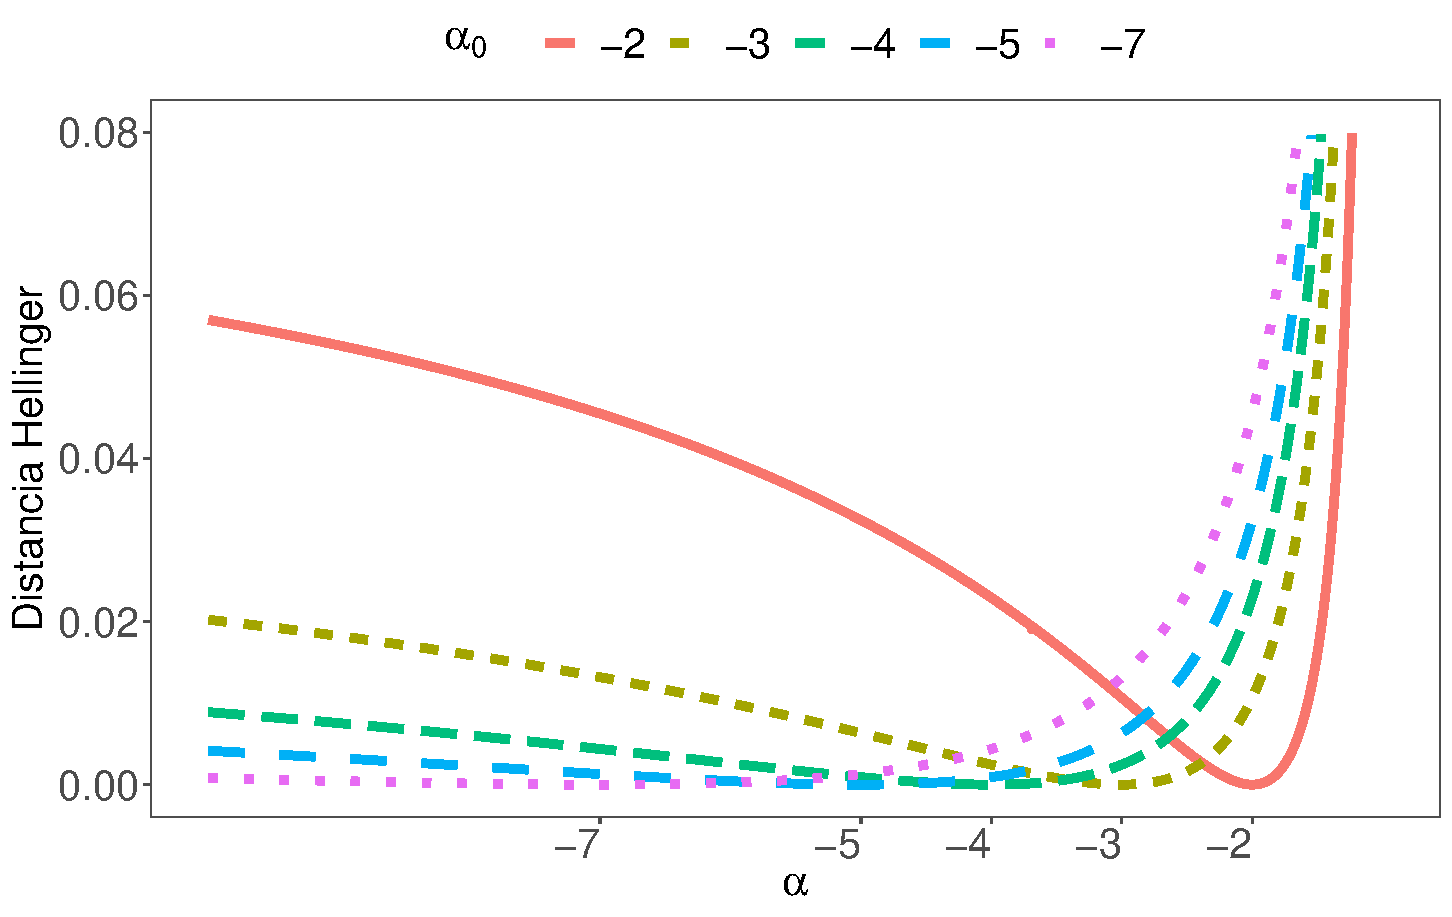
\includegraphics[scale=0.35]{../../Figures/Tesis/Capitulo6/GraficoDHL3_v2.pdf}}
	\subfigure[Rényi]{\includegraphics[scale=0.35]{../../Figures/Tesis/Capitulo6/GraficoDRL3_v2.pdf}}
	\subfigure[Triangular]{\includegraphics[scale=0.35]{../../Figures/Tesis/Capitulo6/GraficoDTL3_v2.pdf}}
	\caption{\label{DistL3}\small Distancias Hellinger, Renyi y Triangular, $\alpha_0= -2,-3,-4,-5,-6,-7$ y $L=3$.}
\end{figure}

\begin{figure}[h!]
	\centering    
	\subfigure[Hellinger]{\includegraphics[scale=0.35]{../../Figures/Tesis/Capitulo6/GraficoDHL8_v2.pdf}}
	\subfigure[Rényi]{\includegraphics[scale=0.35]{../../Figures/Tesis/Capitulo6/GraficoDRL8_v2.pdf}}
	\subfigure[Triangular]{\includegraphics[scale=0.35]{../../Figures/Tesis/Capitulo6/GraficoDTL8_v2.pdf}}
	\caption{\label{DistL8}\small Distancias Hellinger, Renyi y Triangular, $\alpha_0= -2,-3,-4,-5,-6,-7$ y $L=8$.}
\end{figure}

En estos gráficos se puede observar que en todos los casos, cuanto menor es el valor de $\alpha_0$, la curva se hace más plana en un entorno  de él. Esto hace que, al momento de hallar el mínimo, los métodos de optimización sean más inestables y el mínimo sea más difícil de encontrar en forma precisa. Se puede observar también que. a medida que aumenta el valor de $L$, esta situación se revierte y es posible encontrar el mínimo de una forma más eficiente. Recordemos que el número de looks representa la relación señal ruido, por lo tanto, cuanto mayor es el número de looks menor ruido presenta la imagen siendo $L=1$ el caso de mayor ruido. Se puede observar también que la distancia de Hellinger es la que resulta más plana en un entorno del mínimo, y que las distancias de Rényi y Triangular tienen un comportamiento similar.

Siguiendo en la búsqueda de la mejor distancia se realizaron simulaciones Montecarlo para elegir la distancia estocástica que mejor performance tiene a la hora de estimar el parámetro de textura de la distribución $\mathcal{G}_I^0$. En Cassetti et al.~\cite{cassettiast2013} se evaluaron dichas distancias pero ahora estimando el parámetro de textura y  comparando la calidad de estos estimadores con el MV estimador en términos del sesgo y del error cuadrático medio. 

Se realizaron $1000$ replicaciones del experimento que consiste en generar muestras $Z_1, Z_2,\ldots,Z_n$ de variables aleatorias independientes e idénticamente distribuidas donde $Z_i \sim f_{\mathcal{G}_I^0(\alpha,\gamma^*,L)}$ donde el espacio paramétrico está formado por:

\begin{itemize}
	\item Textura: $\alpha=\{-1.5, -3, -5, -8\}$. Con estos valores se describen regiones extramadamente texturadas $(\alpha=-1.5)$, texturadas $(\alpha=\{-3,-5\})$ y homogéneas $(\alpha=-8)$. 
	\item Looks: $L=\{1,3,8\}$, para modelar varios niveles de procesamiento.
	\item Tamaño de muestra: $n=\{9, 25,49, 81,121,1000\}$. 
\end{itemize}

Como se mencionó anteriormente la elección de estos tamaños de muestra se basa en que muchos de los métodos de filtrado de imágenes o detección de bordes utilizan máscaras deslizantes para estimar los parámetros, las cuales suelen ser de tamaño $3 \times 3$,  $5 \times 5$, $7 \times 7$, $9 \times 9$ u  $11 \times 11$. El tamaño de la muestra $n=1000$ se elige para poder estudiar el comportamiento del estimador cuando el tamaño de muestra es grande. 

El valor del parámetro de escala $\gamma^*$ se elige de manera tal que $E(Z)=1$ para que los resultados sean comparables. Esto da una relación entre  $\alpha$ y $\gamma^*$ que es 
\begin{align}
\label{Gama*}
\gamma^*=\alpha-1.
\end{align}
El uso de esta relación nos brinda la posibilidad de llevar un problema de estimación de dos parámetros a estimar un sólo parámetro. 


En cada replicación:
\begin{itemize}
	\item se estima la función de densidad subyacente $\widehat{f}$ utilizando histogramas junto con el método de Freedman Diaconis para elegir el ancho de banda $b$ dado por $b=2 \ \text{IQR}(z_1,\ldots,z_n) n^{-1/3}$ donde $\text{IQR}$ es el rango intercuartil.
	\item se calcula $\widehat{\alpha}= \mathop{\text{argmin}}\limits_{\alpha}d_{\text{D}}(f_{\mathcal{G}_I^0(z,\alpha,1-\alpha,L)},\widehat{f})$ donde D es alguna de las distancias definidas en~\ref{dist}.
\end{itemize} 

De esta manera se obtuvieron $1000$ valores estimados de $\alpha$, $\{\widehat{\alpha}_1, \dots, \widehat{\alpha}_{1000}\}$. Con estos valores se estimó la esperanza, el sesgo y el error cuadrático medio que están definidos por:

\begin{itemize}
	\item $\overline{\widehat{\alpha}}=(1000)^{-1}{\sum_{i=1}^{1000}{\widehat{\alpha}_i}}$
	\item $\widehat{B}(\widehat\alpha) = \overline{\widehat\alpha_i}- \alpha$
	\item $\widehat{\operatorname{\text{ECM}}}=({1000})^{-1}{\sum_{i=1}^{1000}{(\widehat{\alpha}_i-\alpha)^2}}$
\end{itemize}


Las figuras~\ref{ASTalfaL1},~\ref{ASTalfaL2} y~\ref{ASTalfaL3} muestran el sesgo del estimador propuesto para el parámetro de textura $\widehat{\alpha}$ utilizando las distancias de Hellinger, Rényi, Triangular y también Máxima Verosimilitud, para distintos tamaños de muestras $n$ y número de looks $L$. 
La línea recta azul representa el valor verdadero con el que se generaron las muestras. 

En las figuras~\ref{ASTecmL1},~\ref{ASTecmL2} y~\ref{ASTecmL3} se muestra el error cuadrático medio estimado para las mismas combinaciones de parámetros. En este caso la línea azul representa el eje $x$. Los resultados se muestran en escala semilogarítmica para su mejor comprensión visual.
Cabe señalar que la minimización se realizó recorriendo un rango de valores de alfa variando entre $-10$ y $-1$ con paso  $0.1$. 

 En el gráfico de $L=1$ se observa que para zonas texturadas, homogéneas y usando distancia triangular $\widehat{\alpha}$  tiene un comportamiento similiar al MV estimador en términio de sesgo y ECM. Las distancias de Hellinger y Rényi muestran mayor ECM para tamaños de muestra mayores que $9$, salvo para zonas homogéneas donde el ECM es similar en todas las distancias estudiadas. Asimismo estas distancias muestran un mayor sesgo para muestras grandes.

Para el caso de $L=3$ y $L=8$ vemos que tanto el MV estimador y la distancia triangular siguen manteniendo un comportamiento similar para todos los tipos de zonas consideradas. Incluso, en algunos casos el MDE estimador con esta distancia mejora la performance del MV estimador. Se puede observar que las otras distancias presentan un sesgo y un ECM mayor para zonas texturadas y homogéneas. Asimismo, en estos gráficos se observa que los métodos de minimización de distancias poseen menor error para valores grandes del número de looks. 

\begin{figure}[h!]
	\centering    
	\subfigure[\small $\widehat{\alpha}$]{\label{ASTalfaL1}\includegraphics[width=.49\linewidth]{../../Figures/Tesis/Capitulo6/ALFAAST_L1.pdf}}
	\subfigure[\small $\widehat{\text{ECM}}$]{\label{ASTecmL1}\includegraphics[width=.49\linewidth]{../../Figures/Tesis/Capitulo6/ECMAST_L1.pdf}}
	\caption{\small Sesgo y ECM para $\widehat{\alpha}$, L=1.}
\end{figure}	
\begin{figure}[h!]
	\centering
	\subfigure[\small $\widehat{\alpha}$]{\label{ASTalfaL2}\includegraphics[width=.49\linewidth]{../../Figures/Tesis/Capitulo6/ALFAAST_L3.pdf}}
	\subfigure[\small $\widehat{\text{ECM}}$]{\label{ASTecmL2}\includegraphics[width=.49\linewidth]{../../Figures/Tesis/Capitulo6/ECMAST_L3.pdf}}
	\caption{\small Sesgo y ECM para $\widehat{\alpha}$, L=3.}
\end{figure}	
\begin{figure}[h!]
	\centering
	\subfigure[\small $\widehat{\alpha}$]{\label{ASTalfaL3}\includegraphics[width=.49\linewidth]{../../Figures/Tesis/Capitulo6/ALFAAST_L8.pdf}}
	\subfigure[\small $\widehat{\text{ECM}}$]{\label{ASTecmL3}\includegraphics[width=.49\linewidth]{../../Figures/Tesis/Capitulo6/ECMAST_L8.pdf}}
	\caption{\small Sesgo y ECM para $\widehat{\alpha}$, L=8.}
\end{figure}

En Cassetti et al.~\cite{APSAR2013ParameterEstimationStochasticDistances} se aplicó la metodología anterior a una imagen SAR real. En este caso se utilizó una imagen E-SAR~\cite{Horn1996} de un look de los alrededores de Munich, banda L, polarización HH, con $L=1$ en formato intensidad.
E-SAR es un sistema formado por sensores y algoritmos de procesamiento de señales desarrollado, entre otras instituciones, por el centro aeroespacial Deutsches Zentrum für Luft- und Raumfahrt German (DLR), un centro de investigación cuya área principal es la teledetección por microondas.  Principalmente utiliza los sistemas de radar de apertura sintética (SAR), tanto en aire y plataformas aerotransportadas. El compromiso de la institución en los proyectos internacionales ERS-1 y SIR-100 / X-SAR dio origen a los conocidos sistemas aerotransportados SAR y E-SAR. 
%E-SAR opera en las bandas de frecuencia 4, x, C-, L- y P-banda, por lo tanto, cubre un rango de longitudes de onda de 3 a 85 cm. La polarización de la señal de radar es seleccionable, horizontal así como vertical. El modo polarimétrico se conmuta de impulso a impulso en la polarización (HH-HV-W-VH) -secuencia.

En las figuras~\ref{ImagenReales1} y~\ref{ImagenReales1} se muestran dos imágenes E-SAR, de un look, que se utilizaron para testear la performance de las distancias estudiadas y el MV estimador. En ambas figuras se aplicó el método para cada pixel, usando ventanas deslizantes de tamaño $7 \times 7$ y $3 \times 3$ respectivamente. Se puede observar que los resultados son prometedores ya que todas tienen un comportamiento similar y estamos aplicando el método al caso de mayor ruido.


\begin{figure}[H]
	\begin{minipage}[b]{0.45\linewidth} %Una minipágina que cubre la mitad de la página
		\centering
		\subfigure[\label{ImagenReales1} Imagen E-SAR, L=$1$.]{\includegraphics[width=.44\linewidth]{../../Figures/Tesis/Capitulo6/ImHorrible.pdf}}\\
		\subfigure[\label{Real1DH} Hellinger.]{\includegraphics[width=.44\linewidth]{../../Figures/Tesis/Capitulo6/ImHorrible_DH7x7.pdf}}
		\subfigure[\label{Real1DR} R\'enyi, $\beta=0.8$.]{\includegraphics[width=.44\linewidth]{../../Figures/Tesis/Capitulo6/ImHorrible_DR7x7.pdf}}
		\subfigure[\label{Real1DT} Triangular.]{\includegraphics[width=.44\linewidth]{../../Figures/Tesis/Capitulo6/ImHorrible_DT7x7.pdf}}
		\subfigure[\label{Real1MV} MV.]{\includegraphics[width=.44\linewidth]{../../Figures/Tesis/Capitulo6/ImHorrible_MV7x7.pdf}}
		\caption{\small Resultado de estimar el parámetro $\alpha$ para cada pixel, usando ventanas deslizantes de tamaño $7\times 7$.}
	\end{minipage}
\hspace{0.3cm} % Si queremos tener un poco de espacio entre las dos figuras
	\begin{minipage}[b]{0.55\linewidth} %Una minipágina que cubre la mitad de la página
		\centering    
		\subfigure[\label{ImagenReales2} Imagen E-SAR, L=$1$.]{\includegraphics[width=.49\linewidth]{../../Figures/Tesis/Capitulo6/MunichCortadaBien.eps}}\\
		\subfigure[\label{Real2DH} Hellinger.]{\includegraphics[width=.49\linewidth]{../../Figures/Tesis/Capitulo6/MunichCortada3regionesDH.eps}}
		\subfigure[\label{Real2DR} R\'enyi, $\beta=0.8$.]{\includegraphics[width=.49\linewidth]{../../Figures/Tesis/Capitulo6/munichcortada3regionesR.eps}}
		\subfigure[\label{Real2DT} Triangular.]{\includegraphics[width=.49\linewidth]{../../Figures/Tesis/Capitulo6/MunichCortada3regionesDT3x3.eps}}
		\subfigure[\label{Real2MV} MV.]{\includegraphics[width=.49\linewidth]{../../Figures/Tesis/Capitulo6/MunichCortada3RegionesMV.eps}}
		\caption{\small Resultado de estimar el parámetro $\alpha$ para cada pixel, usando ventanas deslizantes de tamaño  $3\times 3$.}
\end{minipage}
\end{figure}
		


Por lo anteriormente expuesto, especialmente por el resulado de las simulaciones, elegimos la distancia Triangular para continuar con el estudio.


\subsection{Incorporando núcleos y evaluando robustez}
\label{jstar}

Como se mencionó en la subsección~\ref{EligiendoDistancias}, en Cassetti et al.~\cite{APSAR2013ParameterEstimationStochasticDistances} se compararon estimadores basados en la distancia de Hellinger, Bhattacharyya, Renyi y Triangular con el MV estimador. Se mostró que la distancia Triangular es la mejor opción para definir el MDE estimador. En ese trabajo se utilizaron histogramas para estimar la función de densidad subyacente $f_S$. En~\cite{gambini2015} %articulo que publicamos en la revista \textit{IEEE Journal of Selected Topics in Applied Earth Observations and Remote Sensing} 
presentamos mejoras con respecto a los resultados obtenidos en~\cite{APSAR2013ParameterEstimationStochasticDistances} ya que: 
\begin{itemize}
	\item Se evaluó el impacto de la contaminación en la estimación de $\widehat{\alpha}$.
	\item Se emplearon núcleos asimétricos en lugar de histogramas para estimar $f_S$.
	\item Se compararon los estimadores basados en la distancia Triangular con el ML estimador, Momentos Fraccionales y LogCumulantes. 
\end{itemize}

Los estimadores por momentos fraccionales han sido usados por~\cite{Frery97,GambiniSC08} en el contexto de estimar el parámetro $\alpha$ para datos de amplitud. Para el caso de datos de intensidad, usando la relación $\gamma^*=-\alpha-1$ en~\ref{momento1medio} se tiene que, $\widehat{\alpha}_\text{Mom12}$, el estimador de $\alpha$ usando momentos fraccionales de orden un medio, es el valor de $\alpha$ que resuelve la ecuación:

\begin{equation}
\frac{1}{n} \sum_{i=1}^n \sqrt{Z_i} -\sqrt{\frac{-\widehat\alpha_{\text{Mom12}}-1}{L}}\frac{\Gamma ( -\widehat\alpha_{\text{Mom12}}-{\frac{1}{2}} )}{ \Gamma (-\widehat\alpha_{\text{Mom12}}) }
\frac{\Gamma (L+{\frac{1}{2}} )}{\Gamma (L)}=0.
\label{estim_moment1_2_gI0}
\end{equation}
donde $Z_1,\ldots,Z_n$ es una muestra de variables aleatorias i.i.d proveniente del modelo $\mathcal{G}_I^0$.

En el capítulo~\ref{metodologia} se indicó que $\widehat{\alpha}_\text{ML}$ y $\widehat{\alpha}_\text{LC}$ son soluciones de las ecuaciones~\ref{rootML} y~\ref{eq:logm} respectivamente.

%En el modelo modelo multiplicativo para el retorno $Z=X \cdot Y$ con datos monopolarizados presentado en la sección XXX, la variable $Y$ que modela el ruido speckle obedece a una distribución $\Gamma(L,L)$, donde $L$ es el número de looks. La retrodisperción $X$ está modelada por una distribución Inversa Gaussiana Generalizada $\mathcal{N}^{-1}( \alpha ,\lambda ,\gamma )$~\cite{Frery97} donde,  para valores particulares de sus parámetros, se obtienen las distribuciones $\Gamma ( \alpha ,\lambda ) $,  $\Gamma ^{-1}( \alpha ,\gamma ) $ e $IG( \gamma ,\lambda ) $ (Gaussiana Inversa) originando que $Z$ esté modelado por las distribuciones $\mathcal{K}$, $\mathcal{G}_I^{0}$ y $\mathcal{G}^{H}$ respectivamente. La distribución $\mathcal{G}^{H}$ fue propuesta en~\cite{harmoniceusar2000} y describe datos  polarimétricos con bastante precisión, aunque
%también se utiliza para imágenes monopolarizadas.

Como se indicó en~\ref{NucleosAsimetricos}, dentro de los núcleos más estudiados se encuentran los núcleos $IG$, $\Gamma$ y Lognormal. Estas distribuciones están presentes en el modelado de datos SAR, ya sea porque son propuestas para describir al backscatter a partir del modelo multiplicativo, o bien porque fueron propuestas como modelo empírico. En el trabajo~\cite{gambini2015} estudiamos la perfomance del núcleo $IG$ para estimar la función de densidad subyacente ($\widehat f_\text{IG}$) en el contexto del MDE estimador y proponemos como estimador del parámetro de textura del modelo $\mathcal{G}_I^0$ a:

\begin{align}
\widehat{\alpha}_{\text{IG}}= \arg\min_{-20\leq \alpha \leq -1} d_{\text{T}}\big(f_{\mathcal{G}^{0}}(\alpha,\gamma^*, L ), \widehat f_\text{IG}(z)\big),
\label{minimization}
\end{align}
donde $d_{\text{T}}$ es la distancia triangular definida en~\ref{triangular} y $\gamma^*=-\alpha-1$.  

Como es sabido, uno de los puntos importantes en estimación no paramétrica de la función de densidad es el ancho de banda. En esta oportunidad y, a través de estudios empíricos, se eligió un ancho de banda fijo $b=\frac{n^{-1/2}}{5}$.

%XXXXXXXXXXXXXXXXXXXXXXXXXXXXXXXXXXXXX

Ninguno de los problemas planteados para encontrar $\widehat{\alpha}$ tiene una solución explícita, por lo tanto apelamos a procedimientos numéricos acordes a cada estimador, para encontrar dichas soluciones. 

Respecto del estimador $\widehat{\alpha}_{{\text{\tiny{MV}}}}$ utilizamos la función $mle$ del software R-project que tiene incorporado el algoritmo L-BFGS-B~\cite{Byrd1995} para encontrar el óptimo de una función de una variable. Este algoritmo es un método de optimización tipo cuasi newton que admite restricciones de borde y es ampliamente utilizado en computación gráfica y computación científica~\cite{Fei2014}. Este algoritmo aproxima al método BFGS (Broyden, Fletcher, Goldfarb y Shanno) ya que no necesita calcular la matriz Hessiana sino que utiliza una apoximación de ella que se actualiza en cada iteración, usando solamente la función y su gradiente. 
Respecto del estimador $\widehat{\alpha}_{{\text{\tiny{LC}}}}$ y $\widehat{\alpha}_{{\text{\tiny{Mom12}}}}$ utilizamos la función $uniroot$ del mismo software que implementa el método de bisección para encontrar el cero de una función.

Un problema que se presenta al momento de estimar el parámetro de textura es la falta de convergencia a una solución global, especialmente en el caso de muestras de pequeño tamaño. Frery et al.~\cite{FreryCribariSouza:JASP:04} and Pianto and Cribari-Neto~\cite{DealingMonotoneLikelihood} propusieron técnicas que tienen como objetivo aliviar este problema, a expensas de un costo computacional alto.

%Un problema que se presenta al momento de estimar el parámetro de textura utilizando las técnicas propuestas incluido ML y aquellos basados en momentos fraccionales~\cite{Frery97} y LogCumulants~\cite{MellinAnalysisPolSAR,BujorTrouveValetNicolas2004,khan2014} es la necesidad de contar con algoritmos iterativos para los cuales no hay garantía de convergencia a una solución global. Esta falta de convergencia sucede en general, en el caso de muestras de pequeño tamaño. Frery et al.~\cite{FreryCribariSouza:JASP:04} and Pianto and Cribari-Neto~\cite{DealingMonotoneLikelihood} propusieron técnicas que tienen como objetivo aliviar este problema, a expensas de un costo computacional alto.

%XXXXXXXXXXXXXXXXXXXXXXXXXXXXXXXXXXXXXXXX

En la figura~\ref{densidades} se muestra el gráfico de la densidad del modelo $\mathcal{G}_I^0$ para valores de $\alpha=\{-20,-25\}$, $\gamma=\gamma^*$, $L=\{3,8\}$. Se puede observar que estas densidades son muy similares ya que la distribución $\mathcal{G}_I^0$ converge en distribución a una $\Gamma(L,L)$~\cite{Frery99} cuando $\alpha \longrightarrow -\infty$ y $\gamma=\gamma^*$. Por este motivo se plantea que $\alpha$ tome valores en el intervalo $[-20,-1]$ en cada método numérico empleado. 

\begin{figure}[H]
	\centering
	\subfigure[L=3]{\includegraphics[width=.45\linewidth]{../../Figures/Tesis/Capitulo6/DensidadGI0L3.pdf}}
	\subfigure[L=8]{\includegraphics[width=.45\linewidth]{../../Figures/Tesis/Capitulo6/DensidadGI0L8.pdf}}
	\caption{\label{densidades}\small Densidad de $\mathcal{G}_I^0(\alpha,\gamma^*,L)$}
\end{figure}


Se realizó un experimento Monte Carlo para evaluar la performance de cada uno de los estimadores propuestos. El espacio parmétrico consiste en una grilla formada por:
\begin{itemize}
	\item tres valores de textura $\alpha=\{-1.5,-3,-5\}$. Los cuales representan áreas texturadas y extremadamente texturadas.
	\item tres niveles de procesamiento señal-ruido $L=\{1,3,8\}$.
	\item tamaños de muestra $n=\{9,25,49,81,121,1000\}$ compatibles con tamaños de ventana $3,\text{ }5,\text{ }7,\text{ }9$.
\end{itemize}

Se generaron $1000$ muestras para cada punto del espacio paramétrico, y se obtuvieron $\{\widehat{\alpha}_1, \dots, \widehat{\alpha}_{1000}\}$ estimaciones para cada una de estas combinaciones. De esta forma se estimaron la media $\overline{\widehat{\alpha}}=(1000)^{-1}{\sum_{i=1}^{1000}{\widehat{\alpha}_i}}$, el sesgo  $\widehat{B}(\widehat\alpha) = \overline{\widehat\alpha_i}- \alpha$ y el error cuadrático medio $\widehat{\operatorname{ECM}}=({1000})^{-1}{\sum_{i=1}^{1000}{(\widehat{\alpha}_i-\alpha)^2}}$ para cada uno de los estimadores estudiados.

En las siguientes figuras ``MV'', ``T'',``Mom12'' and ``LC'' denotarán al estimador basado en el método de Maximum likelihood, distancia Triangular, $\frac{1}{2}$-momento and LogCumulant, respectivamente. En el eje de las abscisas se grafica el tamaño muestral, el cual se presenta en escala semilogarítmica.

Las figuras~\ref{AlfasEstimadosJSTAR2013_L=1},~\ref{AlfasEstimadosJSTAR2013_L=3} y~\ref{AlfasEstimadosJSTAR2013_L=8} muestran la media de $\widehat{\alpha}$ para datos sin contaminar y para diferentes valores de $n$ y $L$. La línea azul representa el verdadero valor de $\alpha$. Se puede observar que $\widehat{\alpha}_{\text{MV}}$ y $\widehat{\alpha}_{\text{DT}}$ tienen un comportamiento similar y se encuentran, en media, cercanos al verdadero valor en la mayoría de los casos estudiados. Es notable el sesgo que presentan  $\widehat{\alpha}_{\text{LC}}$ y $\widehat{\alpha}_{\text{Mom12}}$ para $\alpha=-5$. Se puede observar también que $\widehat\alpha_{\text{ML}}$ tiende a subestimar al verdadero valor de $\alpha$.
Se puede observar que ningún método de estimación tiene el menor error cuadrático medio en todos los casos. El estimador $\widehat{\alpha}_{\text{Mom12}}$ es el que peor se comporta para zonas homogéneas.
%Vasconcellos et al.~\cite{VasconcellosFrerySilva:CompStat} computed a first order approximation of such bias for a closely related model, and our results are in agreement with those.
%The estimator based on the Triangular distance $\widehat\alpha_{\text T}$ compensates this bias.

\begin{figure}[H]
	\centering
	\subfigure[\label{AlfasEstimadosJSTAR2013_L=1}$\widehat{\alpha}$]{\includegraphics[width=.47\linewidth]{../../Figures/Tesis/Capitulo6/GraficoAlfaJstar2013_NoCont_L=1.pdf}}
	\subfigure[\label{ECMEstimadosJSTAR2013_L=1}$\widehat{\text{ECM}}$]{\includegraphics[width=.47\linewidth]{../../Figures/Tesis/Capitulo6/GraficoECMJstar2013_NoCont_L=1.pdf}}
%	\subfigure[\label{AlfasEstimadosJSTAR2013_L=3}$\widehat{\alpha}$, L=3]{\includegraphics[width=.47\linewidth]{../../Figures/Tesis/Capitulo6/GraficoAlfaJstar2013_NoCont_L=3.pdf}}
%	\subfigure[\label{ECMEstimadosJSTAR2013_L=3}$\widehat{\text{ECM}}$, L=3]{\includegraphics[width=.47\linewidth]{../../Figures/Tesis/Capitulo6/GraficoECMJstar2013_NoCont_L=3.pdf}}
	%	\subfigure[\label{AlfasEstimadosJSTAR2013_L=8}$\widehat{\alpha}$, L=8]{\includegraphics[width=.47\linewidth]{../../Figures/Tesis/Capitulo6/GraficoAlfaJstar2013_NoCont_L=8.pdf}}
	%	\subfigure[\label{ECMEstimadosJSTAR2013_L=8}$\widehat{\text{ECM}}$, L=8]{\includegraphics[width=.47\linewidth]{../../Figures/Tesis/Capitulo6/GraficoECMJstar2013_NoCont_L=8.pdf}}
	\caption{\small $\widehat{\alpha}$ y $\widehat{\text{ECM}}$ para datos sin contaminar, $L=1$.}
\end{figure}


\begin{figure}[H]
	\centering
%	\subfigure[\label{AlfasEstimadosJSTAR2013_L=1}$\widehat{\alpha}$, L=1]{\includegraphics[width=.47\linewidth]{../../Figures/Tesis/Capitulo6/GraficoAlfaJstar2013_NoCont_L=1.pdf}}
%	\subfigure[\label{ECMEstimadosJSTAR2013_L=1}$\widehat{\text{ECM}}$, L=1]{\includegraphics[width=.47\linewidth]{../../Figures/Tesis/Capitulo6/GraficoECMJstar2013_NoCont_L=1.pdf}}
	\subfigure[\label{AlfasEstimadosJSTAR2013_L=3}$\widehat{\alpha}$]{\includegraphics[width=.47\linewidth]{../../Figures/Tesis/Capitulo6/GraficoAlfaJstar2013_NoCont_L=3.pdf}}
	\subfigure[\label{ECMEstimadosJSTAR2013_L=3}$\widehat{\text{ECM}}$]{\includegraphics[width=.47\linewidth]{../../Figures/Tesis/Capitulo6/GraficoECMJstar2013_NoCont_L=3.pdf}}
%	\subfigure[\label{AlfasEstimadosJSTAR2013_L=8}$\widehat{\alpha}$, L=8]{\includegraphics[width=.47\linewidth]{../../Figures/Tesis/Capitulo6/GraficoAlfaJstar2013_NoCont_L=8.pdf}}
%	\subfigure[\label{ECMEstimadosJSTAR2013_L=8}$\widehat{\text{ECM}}$, L=8]{\includegraphics[width=.47\linewidth]{../../Figures/Tesis/Capitulo6/GraficoECMJstar2013_NoCont_L=8.pdf}}
	\caption{\small $\widehat{\alpha}$ y $\widehat{\text{ECM}}$ para datos sin contaminar, $L=3$.}
\end{figure}

\begin{figure}[H]
	\centering
%	\subfigure[\label{AlfasEstimadosJSTAR2013_L=1}$\widehat{\alpha}$, L=1]{\includegraphics[width=.47\linewidth]{../../Figures/Tesis/Capitulo6/GraficoAlfaJstar2013_NoCont_L=1.pdf}}
%	\subfigure[\label{ECMEstimadosJSTAR2013_L=1}$\widehat{\text{ECM}}$, L=1]{\includegraphics[width=.47\linewidth]{../../Figures/Tesis/Capitulo6/GraficoECMJstar2013_NoCont_L=1.pdf}}
%	\subfigure[\label{AlfasEstimadosJSTAR2013_L=3}$\widehat{\alpha}$, L=3]{\includegraphics[width=.47\linewidth]{../../Figures/Tesis/Capitulo6/GraficoAlfaJstar2013_NoCont_L=3.pdf}}
%	\subfigure[\label{ECMEstimadosJSTAR2013_L=3}$\widehat{\text{ECM}}$, L=3]{\includegraphics[width=.47\linewidth]{../../Figures/Tesis/Capitulo6/GraficoECMJstar2013_NoCont_L=3.pdf}}
	\subfigure[\label{AlfasEstimadosJSTAR2013_L=8}$\widehat{\alpha}$]{\includegraphics[width=.47\linewidth]{../../Figures/Tesis/Capitulo6/GraficoAlfaJstar2013_NoCont_L=8.pdf}}
	\subfigure[\label{ECMEstimadosJSTAR2013_L=8}$\widehat{\text{ECM}}$]{\includegraphics[width=.47\linewidth]{../../Figures/Tesis/Capitulo6/GraficoECMJstar2013_NoCont_L=8.pdf}}
	\caption{\small $\widehat{\alpha}$ y $\widehat{\text{ECM}}$ para datos sin contaminar, $L=8$.}
\end{figure}

%%%%%%%%%%%%%%%%%%%%%%%%%%%%%%%%%%%%%%%%%%%%%%%%%%%%%%%%%% TIEMPO
Se calculó el tiempo medio de procesamiento, medido en segundos, para cada método y cada caso estudiado. Como  ejemplo se presenta, en la tabla~\ref{tablaDeTiemposmedios}, el tiempo medio para $L=1$ and $n=81$. Se puede observar que nuestra propuesta tiene un mayor costo computacional debido a la integración numérica presente en la definición del estimador. Los otros casos son consistentes con los datos de esta tabla. 
La plataforma informática que se utilizó para realizar los procesos fue Intel(R) Core i7, con 8GB de memoria y 64 bits Windows 7. 

\begin{table}[htb]
	\centering
	\begin{tabular}{cccc}
		\toprule
		MV& DT& Mom$\frac{1}{2}$ & LC \\
		\midrule
		$0.003$& $2.223$ & $0.0001$ &$0.003$ \\
		\bottomrule
	\end{tabular}
\caption{\label{tablaDeTiemposmedios}\small Tiempos medios para datos simulados sin contaminación, $L=1$, $n=81$. }
\end{table}

%%%%%%%%%%%%%%%%%%%%%%%%%%%%%%%%%%%%%%%%%%%%%%%%%%%%%%%%%% ROBUSTEZ
Es muy importante contar con estimadores que sean resistentes a la presencia de datos contaminados, es decir, que sean capaces de producir buenas estimaciones incluso cuando una proporción de los datos no proviene del modelo supuesto como verdadero. Esta situación es de particular importancia en el caso de muestras de pequeño tamaño, por ejemplo, cuando se utilizan filtros que emplean estimadores basados, por lo general, en pequeñas muestras ya que recorren la imagen a través de ventanas deslizantes de tamaño $3 \times 3$, $5 \times 5$ o, por ejemplo, $7 \times 7$. Estas muestras pueden tener datos de zonas con diferentes grado de textura, por ejemplo, en el borde entre diferentes regiones. Esta capacidad de producir buenas estimaciones cuando las observaciones no provienen exactamente del modelo asumido se llama Robustez.

Una de las fuentes de contaminación en las imágenes SAR es el fenómeno de Double Bounce, donde algunos píxeles tienen un alto valor de retorno.  La presencia de tales valores atípicos puede provocar grandes errores en la estimación. La descripción de este fenómeno se hizo en~\ref{DobleBounce}.

Con el fin de evaluar la robustez de los estimadores, proponemos tres escenarios capaces de describir los desvíos del modelo teórico. Para cada uno de estos escenarios generamos muestras contaminadas donde $0<\epsilon \ll 1$ es la proporción de contaminación. 
Sea  $B$ una variable aleatoria Bernoulli con probabilidad $p$ de ocurrencia de la contaminación. Sea $C \in \mathbb R_+$ un valor grande. Entonces
\begin{itemize}
	\item Caso~1:
	Sean $W$ y $U$ variables aleatorias tales que $W \sim \mathcal{G}_I^0(\alpha_1,\gamma_1^*,L)$, y $U \sim \mathcal{G}_I^0(\alpha_2,\gamma_2^*,L) $. Definimos $Z=BU+(1-B)W$, entonces generamos $\{z_1,\dots,z_n\}$ variables aleatorias independientes, idénticamente distribuidas con función de distribución acumulada dada por:
	$$
	(1-\epsilon) \mathcal{F}_{\mathcal{G}_I^0(\alpha_1,\gamma_1^*,L)}(z)+\epsilon\mathcal{F}_{\mathcal{G}_I^0(\alpha_2,\gamma_2^*,L)}(z),
	$$
	donde $\mathcal{F}_{\mathcal{G}_I^0(\alpha,\gamma,L)}$ es la función de distribución acumulada bajo el modelo $\mathcal{G}_I^0(\alpha,\gamma,L)$.
	%
	\item Case~2: Consideramos $W \sim \mathcal{G}_I^0(\alpha_1,\gamma_1^*,L)$ y el retorno definido como $Z=BC+(1-B)W$.
	\item Case~3:
	Consideramos $W \sim \mathcal{G}_I^0(\alpha,\gamma^*,L)$ y $U\sim \mathcal{G}_I^0(\alpha,10^k\gamma^*,L) $ con $k \in \mathbb{N}$. 
	El retorno $Z=BU+(1-B)W$, entonces $\{z_1,\dots,z_n\}$ son variables aleatorias idénticamente distribuidas con función de distribución acumulada dada por: 
	$$
	(1-\epsilon) \mathcal{F}_{\mathcal{G}_I^0(\alpha,\gamma^*,L)}(z)+\epsilon\mathcal{F}_{\mathcal{G}_I^0(\alpha,10^k\gamma^*,L)}(z).
	$$
\end{itemize}

Todos estos modelos consideran desvíos de la hipótesis del modelo teórico. El primer tipo de contaminación asume que, con probabilidad $\epsilon$, los datos pueden provenir de una distribución perteneciente a la familia de distribuciones $\mathcal{G}_I^0$ pero con otros parámetros. El segundo tipo de contaminación modela, con probabilidad $\epsilon$, un retorno con una valor grande y fijo, digamos $C=100$. El tercer tipo de contaminación es un caso particular del primero, donde la contaminación asume que los datos provienen de una distribución cuyo factor de escala es $k$ órdenes de magnitud mayor que el factor de escala correspondiente al modelo teórico. Analizamos estos tres casos de la contaminación en la evaluación de cada estimador.

%%%%%%%%%%%%%%%%%%%%%%%%%%%%%%%%%%%%%%%%%%%%%%%%%%%%%%%%%%%%%
%%% CASE 1, alpha_2 = -15, epsilon = 0.005

Las figuras~\ref{Caso1L1},~\ref{Caso1L3} y~\ref{Caso1L8} muestran $\widehat{\alpha}$ y el error cuadrático medio estimado ($\widehat{\text{ECM}}$) para el Caso $1$ de contaminación con $\alpha_2=-15$, $\epsilon=0.01$, y variando $n$ y $L$.  
Este tipo de contaminación introduce, con probabilidad $\epsilon=0.01$, observaciones casi sin textura en la muestra bajo análisis. Como se espera, la influencia de tal perturbación es más notable en aquella situaciones donde el modelo subyacente está más alejado de la contaminación. Es decir, para valores grandes de $\alpha$. Esto se ve con claridad en las figuras~\ref{ECMContJSTAR2013Caso1_L=1},\ref{ECMContJSTAR2013Caso1_L=3} y \ref{ECMContJSTAR2013Caso1_L=8} donde el $\widehat{\text{ECM}}$ de $\widehat\alpha_{\text{ML}}$, $\widehat\alpha_{\text{Mom12}}$ y $\widehat\alpha_{\text{LC}}$ son mayores que el error cuadrático medio de $\widehat\alpha_{\text T}$ para $L=3,8$, pero esto no es tan claro para el caso de $L=1$. Lo que si se puede decir que $\widehat\alpha_{\text T}$ es competitivo respecto de los otros estimadores para $\alpha=-3,-5$.

\begin{figure}[H]
	\subfigure[\label{AlfasContJSTAR2013Caso1_L=1}$\widehat{\alpha}$]{\includegraphics[width=.48\linewidth]{../../Figures/Tesis/Capitulo6/GraficoAlfaJstar2013_Cont_L=1Caso1.pdf}}
	\subfigure[\label{ECMContJSTAR2013Caso1_L=1}$\widehat{\text{ECM}}$]{\includegraphics[width=.48\linewidth]{../../Figures/Tesis/Capitulo6/GraficoECMJstar2013_Cont_L=1Caso1.pdf}}
%	\subfigure[\label{AlfasContJSTAR2013Caso1_L=3}$\widehat{\alpha}$, L=3]{\includegraphics[width=.48\linewidth]{../../Figures/Tesis/Capitulo6/GraficoAlfaJstar2013_Cont_L=3Caso1.pdf}}
%	\subfigure[\label{ECMContJSTAR2013Caso1_L=3}$\widehat{\text{ECM}}$, L=3]{\includegraphics[width=.48\linewidth]{../../Figures/Tesis/Capitulo6/GraficoECMJstar2013_Cont_L=3Caso1.pdf}}
%	\subfigure[\label{AlfasContJSTAR2013Caso1_L=8}$\widehat{\alpha}$, L=8]{\includegraphics[width=.50\linewidth]{../../Figures/Tesis/Capitulo6/GraficoAlfaJstar2013_Cont_L=8Caso1.pdf}}
%	\subfigure[\label{ECMContJSTAR2013Caso1_L=8}$\widehat{\text{ECM}}$, L=8]{\includegraphics[width=.50\linewidth]{../../Figures/Tesis/Capitulo6/GraficoECMJstar2013_Cont_L=8Caso1.pdf}}
	\caption{\label{Caso1L1}\small Datos contaminados: Caso $1$, $\epsilon=0.01$ y $L=1$.}
\end{figure}

\begin{figure}[H]
%	\subfigure[\label{AlfasContJSTAR2013Caso1_L=1}$\widehat{\alpha}$, L=1]{\includegraphics[width=.48\linewidth]{../../Figures/Tesis/Capitulo6/GraficoAlfaJstar2013_Cont_L=1Caso1.pdf}}
%	\subfigure[\label{ECMContJSTAR2013Caso1_L=1}$\widehat{\text{ECM}}$ ,L=1]{\includegraphics[width=.48\linewidth]{../../Figures/Tesis/Capitulo6/GraficoECMJstar2013_Cont_L=1Caso1.pdf}}
	\subfigure[\label{AlfasContJSTAR2013Caso1_L=3}$\widehat{\alpha}$]{\includegraphics[width=.48\linewidth]{../../Figures/Tesis/Capitulo6/GraficoAlfaJstar2013_Cont_L=3Caso1.pdf}}
	\subfigure[\label{ECMContJSTAR2013Caso1_L=3}$\widehat{\text{ECM}}$]{\includegraphics[width=.48\linewidth]{../../Figures/Tesis/Capitulo6/GraficoECMJstar2013_Cont_L=3Caso1.pdf}}
%	\subfigure[\label{AlfasContJSTAR2013Caso1_L=8}$\widehat{\alpha}$, L=8]{\includegraphics[width=.50\linewidth]{../../Figures/Tesis/Capitulo6/GraficoAlfaJstar2013_Cont_L=8Caso1.pdf}}
%	\subfigure[\label{ECMContJSTAR2013Caso1_L=8}$\widehat{\text{ECM}}$, L=8]{\includegraphics[width=.50\linewidth]{../../Figures/Tesis/Capitulo6/GraficoECMJstar2013_Cont_L=8Caso1.pdf}}
	\caption{\label{Caso1L3}\small Datos contaminados: Caso $1$, $\epsilon=0.01$ y $L=3$.}
\end{figure}

\begin{figure}[H]
%	\subfigure[\label{AlfasContJSTAR2013Caso1_L=1}$\widehat{\alpha}$, L=1]{\includegraphics[width=.48\linewidth]{../../Figures/Tesis/Capitulo6/GraficoAlfaJstar2013_Cont_L=1Caso1.pdf}}
%	\subfigure[\label{ECMContJSTAR2013Caso1_L=1}$\widehat{\text{ECM}}$ ,L=1]{\includegraphics[width=.48\linewidth]{../../Figures/Tesis/Capitulo6/GraficoECMJstar2013_Cont_L=1Caso1.pdf}}
%	\subfigure[\label{AlfasContJSTAR2013Caso1_L=3}$\widehat{\alpha}$, L=3]{\includegraphics[width=.48\linewidth]{../../Figures/Tesis/Capitulo6/GraficoAlfaJstar2013_Cont_L=3Caso1.pdf}}
%	\subfigure[\label{ECMContJSTAR2013Caso1_L=3}$\widehat{\text{ECM}}$, L=3]{\includegraphics[width=.48\linewidth]{../../Figures/Tesis/Capitulo6/GraficoECMJstar2013_Cont_L=3Caso1.pdf}}
	\subfigure[\label{AlfasContJSTAR2013Caso1_L=8}$\widehat{\alpha}$]{\includegraphics[width=.50\linewidth]{../../Figures/Tesis/Capitulo6/GraficoAlfaJstar2013_Cont_L=8Caso1.pdf}}
	\subfigure[\label{ECMContJSTAR2013Caso1_L=8}$\widehat{\text{ECM}}$]{\includegraphics[width=.50\linewidth]{../../Figures/Tesis/Capitulo6/GraficoECMJstar2013_Cont_L=8Caso1.pdf}}
	\caption{\label{Caso1L8}\small Datos contaminados: Caso $1$, $\epsilon=0.01$ y $L=8$.}
\end{figure}

%%%%%%%%%%%%%%%%%%%%%%%%%%%%%%%%%%%%%%%%%%%%%%%%%%%%%%%%%%%%%%%
%%% CASE 2, alpha_2 = -15, epsilon = 0.001, C = 100

Las figuras~\ref{Caso2L1},~\ref{Caso2L3} y~\ref{Caso2L8} presentan $\widehat{\alpha}$ y $\widehat{\text{ECM}}$ para el Caso $2$ de contaminación con $\epsilon=0.001$ y $C=100$. Este tipo de contaminación injecta un valor constante, en este caso $100$, con probabilidad $\epsilon=0.001$. Como estamos considerando muestras con media unitaria, este valor de $C$ respresenta un valor grande de contaminación. En este caso $\widehat\alpha_{\text T}$ es, en media, más cercano al verdadero valor que los otros métodos, y el valor de $\widehat{\text{ECM}}$ es menor.

\begin{figure}[h!]
	\subfigure[\label{AlfasContJSTAR2013Caso2_L=1}$\widehat{\alpha}$]{\includegraphics[width=.48\linewidth]{../../Figures/Tesis/Capitulo6/GraficoAlfaJstar2013_Cont_L=1Caso1.pdf}}
	\subfigure[\label{ECMContJSTAR2013Caso2_L=1}$\widehat{\text{ECM}}$]{\includegraphics[width=.48\linewidth]{../../Figures/Tesis/Capitulo6/GraficoECMJstar2013_Cont_L=1Caso1.pdf}}
%	\subfigure[\label{AlfasContJSTAR2013Caso2_L=3}$\widehat{\alpha}$, L=3]{\includegraphics[width=.48\linewidth]{../../Figures/Tesis/Capitulo6/GraficoAlfaJstar2013_Cont_L=3Caso1.pdf}}
%	\subfigure[\label{ECMContJSTAR2013Caso2_L=3}$\widehat{\text{ECM}}$, L=3]{\includegraphics[width=.48\linewidth]{../../Figures/Tesis/Capitulo6/GraficoECMJstar2013_Cont_L=3Caso1.pdf}}
%	\subfigure[\label{AlfasContJSTAR2013Caso2_L=8}$\widehat{\alpha}$, L=8]{\includegraphics[width=.50\linewidth]{../../Figures/Tesis/Capitulo6/GraficoAlfaJstar2013_Cont_L=8Caso1.pdf}}
%	\subfigure[\label{ECMContJSTAR2013Caso2_L=8}$\widehat{\text{ECM}}$, L=8]{\includegraphics[width=.50\linewidth]{../../Figures/Tesis/Capitulo6/GraficoECMJstar2013_Cont_L=8Caso1.pdf}}
	\caption{\label{Caso2L1}\small Datos contaminados: Caso $2$, $\epsilon=0.001$ y $L=1$.}
\end{figure}

\begin{figure}[h!]
%	\subfigure[\label{AlfasContJSTAR2013Caso2_L=1}$\widehat{\alpha}$, L=1]{\includegraphics[width=.48\linewidth]{../../Figures/Tesis/Capitulo6/GraficoAlfaJstar2013_Cont_L=1Caso1.pdf}}
%	\subfigure[\label{ECMContJSTAR2013Caso2_L=1}$\widehat{\text{ECM}}$ ,L=1]{\includegraphics[width=.48\linewidth]{../../Figures/Tesis/Capitulo6/GraficoECMJstar2013_Cont_L=1Caso1.pdf}}
	\subfigure[\label{AlfasContJSTAR2013Caso2_L=3}$\widehat{\alpha}$, L=3]{\includegraphics[width=.48\linewidth]{../../Figures/Tesis/Capitulo6/GraficoAlfaJstar2013_Cont_L=3Caso1.pdf}}
	\subfigure[\label{ECMContJSTAR2013Caso2_L=3}$\widehat{\text{ECM}}$, L=3]{\includegraphics[width=.48\linewidth]{../../Figures/Tesis/Capitulo6/GraficoECMJstar2013_Cont_L=3Caso1.pdf}}
%	\subfigure[\label{AlfasContJSTAR2013Caso2_L=8}$\widehat{\alpha}$, L=8]{\includegraphics[width=.50\linewidth]{../../Figures/Tesis/Capitulo6/GraficoAlfaJstar2013_Cont_L=8Caso1.pdf}}
%	\subfigure[\label{ECMContJSTAR2013Caso2_L=8}$\widehat{\text{ECM}}$, L=8]{\includegraphics[width=.50\linewidth]{../../Figures/Tesis/Capitulo6/GraficoECMJstar2013_Cont_L=8Caso1.pdf}}
	\caption{\label{Caso2L3}\small Datos contaminados: Caso $2$, $\epsilon=0.001$ y $L=3$.}
\end{figure}

\begin{figure}[H]
%	\subfigure[\label{AlfasContJSTAR2013Caso2_L=1}$\widehat{\alpha}$, L=1]{\includegraphics[width=.48\linewidth]{../../Figures/Tesis/Capitulo6/GraficoAlfaJstar2013_Cont_L=1Caso1.pdf}}
%	\subfigure[\label{ECMContJSTAR2013Caso2_L=1}$\widehat{\text{ECM}}$ ,L=1]{\includegraphics[width=.48\linewidth]{../../Figures/Tesis/Capitulo6/GraficoECMJstar2013_Cont_L=1Caso1.pdf}}
%	\subfigure[\label{AlfasContJSTAR2013Caso2_L=3}$\widehat{\alpha}$, L=3]{\includegraphics[width=.48\linewidth]{../../Figures/Tesis/Capitulo6/GraficoAlfaJstar2013_Cont_L=3Caso1.pdf}}
%	\subfigure[\label{ECMContJSTAR2013Caso2_L=3}$\widehat{\text{ECM}}$, L=3]{\includegraphics[width=.48\linewidth]{../../Figures/Tesis/Capitulo6/GraficoECMJstar2013_Cont_L=3Caso1.pdf}}
	\subfigure[\label{AlfasContJSTAR2013Caso2_L=8}$\widehat{\alpha}$, L=8]{\includegraphics[width=.50\linewidth]{../../Figures/Tesis/Capitulo6/GraficoAlfaJstar2013_Cont_L=8Caso1.pdf}}
	\subfigure[\label{ECMContJSTAR2013Caso2_L=8}$\widehat{\text{ECM}}$, L=8]{\includegraphics[width=.50\linewidth]{../../Figures/Tesis/Capitulo6/GraficoECMJstar2013_Cont_L=8Caso1.pdf}}
	\caption{\label{Caso2L8}\small Datos contaminados: Caso $2$, $\epsilon=0.001$  y $L=8$.}
\end{figure}
%%% CASE 3, epsilon 0.001, k = 2

Las figuras~\ref{Caso3L1},~\ref{Caso3L3} y~\ref{Caso3L8} muestran $\widehat{\alpha}$ y $\widehat{\text{ECM}}$ para el Caso 3 de contaminación con $\epsilon=0.005$ y $k=2$. En este caso se contamina la muestra proveniente del modelo verdadero con un observaciones que, con probabilidad $\epsilon=0.005$, provienen de una distribución $\mathcal G_I^0$ con un factor de escala cien veces más grande que el correspondiente al modelo verdadero. El comportamiento de estos estimadores sigue el mismo patrón para $L=3 \text{ y } 8$: $\widehat\alpha_{\text T}$ produce estimaciones más cercanas al verdadero valor con un ECM más chico. No hay un buen estimador para el caso $L=1$ en este caso de contaminación.

\begin{figure}[h!]
	\subfigure[\label{AlfasContJSTAR2013Caso3_L=1}$\widehat{\alpha}$]{\includegraphics[width=.48\linewidth]{../../Figures/Tesis/Capitulo6/GraficoAlfaJstar2013_Cont_L=1Caso3.pdf}}
	\subfigure[\label{ECMContJSTAR2013Caso3_L=1}$\widehat{\text{ECM}}$]{\includegraphics[width=.48\linewidth]{../../Figures/Tesis/Capitulo6/GraficoECMJstar2013_Cont_L=1Caso3.pdf}}
%	\subfigure[\label{AlfasContJSTAR2013Caso3_L=3}$\widehat{\alpha}$, L=3]{\includegraphics[width=.48\linewidth]{../../Figures/Tesis/Capitulo6/GraficoAlfaJstar2013_Cont_L=3Caso3.pdf}}
%	\subfigure[\label{ECMContJSTAR2013Caso3_L=3}$\widehat{\text{ECM}}$, L=3]{\includegraphics[width=.48\linewidth]{../../Figures/Tesis/Capitulo6/GraficoECMJstar2013_Cont_L=3Caso3.pdf}}
%	\subfigure[\label{AlfasContJSTAR2013Caso3_L=8}$\widehat{\alpha}$, L=8]{\includegraphics[width=.50\linewidth]{../../Figures/Tesis/Capitulo6/GraficoAlfaJstar2013_Cont_L=8Caso3.pdf}}
%	\subfigure[\label{ECMContJSTAR2013Caso3_L=8}$\widehat{\text{ECM}}$, L=8]{\includegraphics[width=.50\linewidth]{../../Figures/Tesis/Capitulo6/GraficoECMJstar2013_Cont_L=8Caso3.pdf}}
	\caption{\label{Caso3L1}\small Datos contaminados: Caso $3$, $\epsilon=0.005$ y $ L=1$.}
\end{figure}

\begin{figure}[h!]
%	\subfigure[\label{AlfasContJSTAR2013Caso3_L=1}$\widehat{\alpha}$, L=1]{\includegraphics[width=.48\linewidth]{../../Figures/Tesis/Capitulo6/GraficoAlfaJstar2013_Cont_L=1Caso3.pdf}}
%	\subfigure[\label{ECMContJSTAR2013Caso3_L=1}$\widehat{\text{ECM}}$ ,L=1]{\includegraphics[width=.48\linewidth]{../../Figures/Tesis/Capitulo6/GraficoECMJstar2013_Cont_L=1Caso3.pdf}}
	\subfigure[\label{AlfasContJSTAR2013Caso3_L=3}$\widehat{\alpha}$]{\includegraphics[width=.48\linewidth]{../../Figures/Tesis/Capitulo6/GraficoAlfaJstar2013_Cont_L=3Caso3.pdf}}
	\subfigure[\label{ECMContJSTAR2013Caso3_L=3}$\widehat{\text{ECM}}$]{\includegraphics[width=.48\linewidth]{../../Figures/Tesis/Capitulo6/GraficoECMJstar2013_Cont_L=3Caso3.pdf}}
%	\subfigure[\label{AlfasContJSTAR2013Caso3_L=8}$\widehat{\alpha}$, L=8]{\includegraphics[width=.50\linewidth]{../../Figures/Tesis/Capitulo6/GraficoAlfaJstar2013_Cont_L=8Caso3.pdf}}
%	\subfigure[\label{ECMContJSTAR2013Caso3_L=8}$\widehat{\text{ECM}}$, L=8]{\includegraphics[width=.50\linewidth]{../../Figures/Tesis/Capitulo6/GraficoECMJstar2013_Cont_L=8Caso3.pdf}}
	\caption{\label{Caso3L3}\small Datos contaminados: Caso $3$, $\epsilon=0.005$ y $ L=3$.}
\end{figure}

\begin{figure}[H]
%	\subfigure[\label{AlfasContJSTAR2013Caso3_L=1}$\widehat{\alpha}$, L=1]{\includegraphics[width=.48\linewidth]{../../Figures/Tesis/Capitulo6/GraficoAlfaJstar2013_Cont_L=1Caso3.pdf}}
%	\subfigure[\label{ECMContJSTAR2013Caso3_L=1}$\widehat{\text{ECM}}$ ,L=1]{\includegraphics[width=.48\linewidth]{../../Figures/Tesis/Capitulo6/GraficoECMJstar2013_Cont_L=1Caso3.pdf}}
%	\subfigure[\label{AlfasContJSTAR2013Caso3_L=3}$\widehat{\alpha}$, L=3]{\includegraphics[width=.48\linewidth]{../../Figures/Tesis/Capitulo6/GraficoAlfaJstar2013_Cont_L=3Caso3.pdf}}
%	\subfigure[\label{ECMContJSTAR2013Caso3_L=3}$\widehat{\text{ECM}}$, L=3]{\includegraphics[width=.48\linewidth]{../../Figures/Tesis/Capitulo6/GraficoECMJstar2013_Cont_L=3Caso3.pdf}}
	\subfigure[\label{AlfasContJSTAR2013Caso3_L=8}$\widehat{\alpha}$]{\includegraphics[width=.50\linewidth]{../../Figures/Tesis/Capitulo6/GraficoAlfaJstar2013_Cont_L=8Caso3.pdf}}
	\subfigure[\label{ECMContJSTAR2013Caso3_L=8}$\widehat{\text{ECM}}$]{\includegraphics[width=.50\linewidth]{../../Figures/Tesis/Capitulo6/GraficoECMJstar2013_Cont_L=8Caso3.pdf}}
	\caption{\label{Caso3L8}\small Datos contaminados: Caso $3$, $\epsilon=0.005$ y $ L=8$.}
\end{figure}

Como se mencionó anteriormente, los algoritmos implementados para los casos de los estimadores Mom12 y LogCumulant no convergen en algunos casos. En el experimento Monte Carlo, si Mom12 o LogCumulant no convergen, eliminamos los estimadores calculados con los otros métodos en esa iteración, por lo que la cantidad de elementos para calcular $\overline{\widehat{\alpha}}$, el sesgo y el error cuadrático medio es menor que $1000$.

La tabla~\ref{tabla_removidos} informa, a modo de ejemplo, el porcentaje de casos que fueron removidos para el Caso $1$ y $\alpha_2 = -15, \epsilon = 0.01$. Estos resultados son consistentes con los otras escenarios de contaminación, y sugieren que estos métodos son progresivamente más propensos a fallar en casos con mayor presencia de ruido speckle.

\begin{table}[hbt]
	\centering
	\begin{tabular}{ccc}
		\toprule
		$L$ & Mom12  & LC \\
		\midrule
		$1$ & $22.87$  & $21.56$ \\
		$3$ & $11.71$  &  $11.87$ \\
		$8$ & $5.81$ & $6.04$  \\
		\bottomrule
	\end{tabular}
\caption{\label{tabla_removidos}Porcentaje de casos de no convergencia para los estimadores de Momentos y LogCumulant en el Caso 1, $\alpha_2 = -15, \epsilon = 0.01$}
\end{table}


%\begin{figure}[h!]
%	\centering
%	\subfigure[\label{AlfasContJSTAR2013Caso1_L=1}$\widehat{\alpha}$]{\includegraphics[width=.48\linewidth]{../../Figures/Tesis/Capitulo6/GraficoAlfaJstar2013_Cont_L=1Caso1.pdf}}
%	\subfigure[\label{ECMContJSTAR2013Caso1_L=1}ECM]{\includegraphics[width=.48\linewidth]{../../Figures/Tesis/Capitulo6/GraficoECMJstar2013_Cont_L=1Caso1.pdf}}
%	\caption{\small Datos contaminados: Caso1, L=1.}
%\end{figure}
%
%\begin{figure}[h!]
%	\centering
%	\subfigure[\label{AlfasContJSTAR2013Caso1_L=3}$\widehat{\alpha}$]{\includegraphics[width=.47\linewidth]{../../Figures/Tesis/Capitulo6/GraficoAlfaJstar2013_Cont_L=3Caso1.pdf}}
%	\subfigure[\label{ECMContJSTAR2013Caso1_L=3}ECM]{\includegraphics[width=.47\linewidth]{../../Figures/Tesis/Capitulo6/GraficoECMJstar2013_Cont_L=3Caso1.pdf}}
%	\caption{\small Datos contaminados: Caso1, L=3.}
%\end{figure}
%
%\begin{figure}[h!]
%	\centering
%	\subfigure[\label{AlfasContJSTAR2013Caso1_L=8}$\widehat{\alpha}$]{\includegraphics[width=.47\linewidth]{../../Figures/Tesis/Capitulo6/GraficoAlfaJstar2013_Cont_L=8Caso1.pdf}}
%	\subfigure[\label{ECMContJSTAR2013Caso1_L=8}ECM]{\includegraphics[width=.47\linewidth]{../../Figures/Tesis/Capitulo6/GraficoECMJstar2013_Cont_L=8Caso1.pdf}}
%	\caption{\small Datos contaminados: Caso1, L=8.}
%\end{figure}
%\begin{figure}[h!]
%	\centering
%	\subfigure[\label{AlfasEstimadosJSTAR2013_L=3}$\widehat{\alpha}$]{\includegraphics[width=.47\linewidth]{../../Figures/Tesis/Capitulo6/GraficoAlfaJstar2013NoContL=3.pdf}}
%	\subfigure[\label{ECMEstimadosJSTAR2013_L=3}ECM]{\includegraphics[width=.47\linewidth]{../../Figures/Tesis/Capitulo6/GraficoECMJstar2013NoContL=3.pdf}}
%	\caption{\small  Datos sin contaminar, L=3.}
%\end{figure}
%
%\begin{figure}[h!]
%	\subfigure[\label{AlfasEstimadosJSTAR2013_L=8}$\widehat{\alpha}$]{\includegraphics[width=.47\linewidth]{../../Figures/Tesis/Capitulo6/GraficoAlfaJstar2013NoContL=8.pdf}}
%	\subfigure[\label{ECMEstimadosJSTAR2013_L=8}ECM]{\includegraphics[width=.47\linewidth]{../../Figures/Tesis/Capitulo6/GraficoECMJstar2013NoContL=8.pdf}}
%	\caption{\small Datos sin contaminar, L=8.}
%\end{figure}

Hemos aplicado estos métodos en una imagen real, la misma imagen utilizada en Cassetti et al.~\cite{APSAR2013ParameterEstimationStochasticDistances}, una imagen E-SAR~\cite{Horn1996} de un look de los alrededores de Munich, banda L, polarización HH en formato intensidad. La figura~\ref{reales2} muestra las regiones usadas para estimar el parámetro de textura. Esta imagen tiene $300\times250$ pixels y comprende principalmente dos áreas de cultivo diferentes.

\begin{figure}[h!]
	\centering
	\includegraphics[width=.52\linewidth,angle=-90]{../../Figures/Tesis/Capitulo6/MunchCortadaReg.pdf}
	\caption{\label{reales2}Image real E-SAR junto con la regiones usadas para estimar el parámetro $\alpha$.}
\end{figure}

La tabla~\ref{resultadosalfaEstim} muestra los resultados de las estimaciones del parámetro $\alpha$ para cada región rectangular junto con los tiempos de procesamiento, donde $NA$ significa que no fue posible estimar el correspondiente estimador ya que el algoritmo no convergió. El resto de las estimaciones arrojan valores compatibles con el mismo tipo de zona en cada una de las muestras analizadas.

\begin{table}[h!]
	\centering
	\begin{tabular}{c*9{c}}
		\toprule
		\multirow{2 }{*} {Color} & \multirow{2 }{*}{n} & \multirow{2 }{*}{$\widehat{\alpha}_{\text MV}$} & \multirow{2 }{*}{$\widehat\alpha_{\text T}$} & \multirow{2 }{*}{$\widehat\alpha_{\text{Mom12}}$} & \multirow{2 }{*}{$\widehat\alpha_{\text{LC}}$} & \small Tiempo  &  \small Tiempo & \small Tiempo &  \small Tiempo  \\
		&      &                        &                           &                                 &                                &  \small MV &  \small DT &   \small Mom12 &  LC \\
		\midrule
		Magenta   & $100$  & $-1.9$ & $-2.7$ & $-1.9$  & $-1.7$  & $0.03$ & $5.85$ & $0.03$  & $0.02$\\
		Amarillo  & $90$   & $-6.2$ & $-5.1$ & $-6.6$  & $-6.8$  & $0.00$ &$5.16$  & $0.00$  & $0.00$\\
		Rojo      & $64$   & $-1.8$ & $-1.9$ & $-1.9$  & $-1.8$  & $ 0.00 $&$4.17$ & $0.00$  & $0.00$\\
		Verde     & $48$   & $-2.5$ & $-2.5$ & $-2.9$  & $-3.1$  & $0.00$ & $3.31$ & $ 0.00$ & $0.00$\\
		Azul      & $25$   & $-4.9$ & $-3.0$ &  $NA$   & $NA$    & $0.00$ & $2.08$ & $0.00$  & $0.00$\\
		\bottomrule
	\end{tabular}
\caption{\label{resultadosalfaEstim}$\widehat{\alpha}$ para las muestras de la figura~\ref{reales2}.}
\end{table}

Aplicamos el test de Kolmogorov-Smirnov (KS-test) como otra estrategia para evaluar a los estimadores bajo estudio. Se aplicó el test a dos muestras: una muestra $\bm x$ que proviene de la imagen, y una segunda muestra $\bm y$ simulada.
Babu and Feigelson~\cite{Jogesh2006} alertan sobre el uso de la misma muestra para estimar los parámetros y para realizar el KS test, porque se pueden sacar conclusiones erróneas. Entonces tomamos una muestra de la imagen real $\bm x$ usada para estimar los parámetros con los cuatro métodos bajo análisis y la comparamos con una muestra simulada $\bm y$, del mismo tamaño, proveniente de una distribución $\mathcal G_I^0$ con los parámetros estimados. Se aplicó el KS test entre $\bm x$ y $\bm y$ considerando la hipótesis nula $H_0$ ``ambas muestras provienen de la misma distribución'', y el complemento de esta hipótesis como hipótesis alternativa.

La tabla~\ref{resultadosTestMunich} muestra los $p$-valores. Se puede observar que no hay suficiente evidencia para rechazar la hipótesis nula con un nivel de signficación del $5$\% en cualquiera de los casos.
%This result justifies the adequacy of the model for the data.
%Se aplica  el test de Kolmogorov Smirnov utilizando dos muestras de datos $X$ e $Y$. La muestra $X$ proviene de la imagen real (cuyo número equivalente de looks $L$ es conocido), de tamaño $n$. Luego se estima el parámetro $\hat{\alpha}$ utilizando esta muestra. Luego se genera una muestra simulada $Y$ con distribución $\mathcal{G}^0_I(\hat{\alpha},n,L)$ y se calcula el test de hipótesis $K-S$ con la hipótesis nula $H_0= \text{Ambas muestras poseen la misma distribución}$ y $H_A= \text{Las muestras no poseen la misma distribución}$. La siguiente tambla muestra los resultados de los p-valores obtenidos. Se observa que no se rechaza la hipótesis nula en ninguno de los casos.

\begin{table}[h!]
	\centering
	\begin{tabular}{c*4{c}}
		\toprule
		Color      & TestMV    & TestDT    & TestMom12  &TestLC \\
		\midrule
		Magenta    & $0.46$    & $ 0.58$   & $0.28$   & $0.69$\\
		Amarillo   & $0.63$    & $0.98$    & $0.76$   & $0.22$\\
		Rojo       & $0.30$    & $ 0.30$   & $0.21$   & $0.99$\\
		Verde      & $0.37$    & $0.85$    & $0.37$   & $0.37$\\
		Azul       & $0.15$    & $0.07$    & $NA $    & $NA $\\
		\bottomrule
	\end{tabular}
\caption{\label{resultadosTestMunich} $p$-valor del KS test para las muestras de la imagen de la figura~\ref{reales2}.}
\end{table}

La figura~\ref{ImagenCornerReflector} muestra una imagen con la presencia de un corner reflector, mientras que la figura~\ref{MuestrasCorner} muestra las regiones usadas para estimar el parámetro de textura para esta situcación. La tabla~\ref{resultadosCorner} presenta los valores de  $\widehat{\alpha}$ para cada área rectangular en la imagen de la figura~\ref{MuestrasCorner}.

Los estimadores MV, Mom12 y LogCumulant son incapaces de producir una estimación en pequeñas muestras.  Se puede observar que tanto $\widehat\alpha_{\text{Mom12}}$ como $\widehat\alpha_{\text{LC}}$ requieren al menos un tamaño de muestra de $90$ observaciones para que se pueda dar una estimación para $\alpha$. El estimador basado en la distancia triangular produce valores plausibles bajo contaminación incluso con muestras muy pequeñas.

\begin{figure}[H]
	\centering
	\includegraphics[angle =90,width=.8\linewidth]{../../Figures/Tesis/Capitulo6/Corner.pdf}
	\caption{\label{ImagenCornerReflector} Imagen real SAR de $1$-look con un corner reflector.}
\end{figure}

\begin{figure}[H]
	\centering
	%\subfigure[Single-look E-SAR imagen con un corner reflector.]{\includegraphics[angle =90,width=.8\linewidth]{../../Figures/Tesis/Capitulo6/Corner.pdf}}
	%\subfigure[\label{Cornerregiones} Regiones de interés.]{\includegraphics[angle =90,width=.8\linewidth,]{../../Figures/Tesis/Capitulo6/CornerReg}}
	\includegraphics[angle =90,width=.8\linewidth,]{../../Figures/Tesis/Capitulo6/CornerReg}
	\caption{\label{MuestrasCorner} Muestras de varios tamaños en una imagen real SAR de $1$-look con un corner reflector.}
\end{figure}

\begin{table}[H]
	\centering
	\caption{\label{resultadosCorner}$\widehat{\alpha}$ y tiempos de procesos para las muestras presentadas en la figura~\ref{MuestrasCorner}}
	\begin{tabular}{c*9{c}}
	\toprule
	\multirow{2 }{*} {Color} & \multirow{2 }{*}{n} & \multirow{2 }{*}{$\widehat\alpha_{\text MV}$} & \multirow{2 }{*}{$\widehat\alpha_{\text T}$} & \multirow{2 }{*}{$\widehat\alpha_{\text{Mom12}}$} & \multirow{2 }{*}{$\widehat\alpha_{\text{LC}}$} & \small Tiempo  &  \small Tiempo & \small Tiempo &  \small Tiempo  \\
	&      &                        &                           &                                 &                                &  \small MV &  \small DT &   \small Mom12 &  LC \\
	\midrule
		Magenta     & $15$  & $-20.0$ & $-4.1$  & $NA $   & $NA $     &  $0.03$  &  $ 1.95 $    &  $ 0.03$   &  $0.03$ \\
		Verde       & $42$  & $-9.2$  & $-5.0$  & $NA$    & $ NA $    &  $0.00$  &  $ 4.04$     &  $ 0.00$   &  $ 0.00$\\
		Azul        & $90$  & $-3.5$  & $-2.7$  & $-4.7$  & $-14.2$   &  $0.02$  &  $4.85$      &  $ 0.00$   &  $0.00$\\
		Amarillo    & $156$ & $-2.2$  & $-1.8$  & $-2.6$  & $-3.4$    &  $0.01$  &  $8.35$      &  $0.00$    &  $0.00$\\
		Rojo        & $225$ & $-1.9 $ & $-1.7$  & $-2.1$  & $ -2.5 $  &  $0.02$  & $ 10.97$     &  $ 0.00$   &  $0.00$\\
		\bottomrule
	\end{tabular}
\end{table}

La tabla~\ref{pvaluesTrueNestedSamples} presenta los $p$-valores del KS test aplicado a las muestras señaladas en la figura~\ref{MuestrasCorner}. Como se mencionó anteriormente el $\widehat\alpha_{\text{Mom12}}$ y $\widehat\alpha_{\text{LC}}$ no pudieron producir estimaciones en dos muestras y, por lo tanto, no fue posible aplicar el test. Cabe señalar que  se rechaza la hipótesis nula: las muestras provienen de la misma distribución, para la muestra azul y el MV estimador, y para la muestra roja que es la de mayor tamaño para los estimadores $\widehat\alpha_{\text{Mom12}}$ y $\widehat\alpha_{\text{LC}}$. 

Estos resultados nos llevan a concluir que el modelo $\mathcal{G}_I^0$ es una buena opción para modelar adecuadamente datos provenientes de imágenes SAR con datos de intensidad ante la presencia de contaminación. Asimismo podemos concluir que el estimador propuesto es una buena elección para estimar el parámetro de textura de la distribución $\mathcal{G}_I^0$, ya que es competitivo frente al MV estimador y mejora a los otros dos estimadores estudiados especialmente para el caso de muestras de pequeño tamaño.

\begin{table*}[htb]
	\centering
	\caption{\label{pvaluesTrueNestedSamples} $p$-valores del KS test para la muestras indicadas en la figura~\ref{MuestrasCorner}.}
	\begin{tabular}{c*4{r}}
		\toprule
		Color       &  TestMV    &  TestDT    &  TestMom12  &  TestLC\\
		\midrule
		Magenta     & $ 0.38$    & $ 0.93 $   & $ NA $     & $  NA$\\
		Verde       & $ 0.11$    & $ 0.93$    & $ NA $     & $   NA$\\
		Azul        & $ 0.01 $   & $0.11 $    & $ 0.40$    & $ 0.11$\\
		Amarillo    & $0.19$     & $0.31$     & $ 0.46 $   & $0.15$\\
		Rojo        & $0.23$     & $0.12$     & $ 0.008$   & $0.02$\\
		\bottomrule
	\end{tabular}
\end{table*}
%\begin{table}[hbt]
%	\centering
%	\caption{Número de casos de no convergencia para distancia triangular generalizada, L=$3$}
%	\label{NoConvDTG}
%		\begin{tabular}{c*7{r}}
%			\toprule		
%			$\alpha$ & $n$ & s=$1$ & s=$1.5$ & s=$2$ & s=$3$ & s=$4$\\
%			\midrule
%			\multirow{3 }{*}{$-1.5$} 
%			& $9$  & $26$ & $14$ & $11$ & $7$ & $6$ \\ 
%			& $25$ & $0 $ & $0 $ & $0$  & $0$ & $0$\\ 
%			& $49$ & $0$  & $1 $ & $1$  & $0$ & $0$\\ 
%			\midrule
%			\multirow{3 }{*}{$-3$}
%			& $9$  & $10$ & $6 $ & $5$  & $4$ & $4$ \\ 
%			& $25$ & $0$  & $1 $ & $1$  & $1$ & $0$\\ 
%			& $49$ & $0$  & $0$  & $0$  & $0$ & $0$\\ 
%			\midrule
%			\multirow{3 }{*}{$-5$} 
%			& $9$  & $4 $ & $3 $ & $3$  & $2$ & $1$\\ 
%			& $25$ & $1 $ & $1 $ & $1$  & $0$ & $0$\\ 
%			& $49$ & $0$  & $0 $ & $0$  & $0$ & $0$\\ 
%			\midrule
%			\multirow{3 }{*}{$-8$} 
%			& $0$ & $0$ & $0$ & $0$  & $0$ & $0$\\ 
%			& $0$ & $0$ & $0$ & $0$  & $0$ & $0$\\ 
%			& $0$ & $0$ & $0$ & $0$  & $0$ & $0$\\ 
%			\midrule
%			\bottomrule 	
%		\end{tabular}
%\end{table}	

\subsection{Mejorando la propuesta}
\label{mejorando}

Para el caso $L=1$ la distribución $\mathcal{G}_I^0(\alpha,\gamma)$ es una distribución de Pareto Generalizada de parámetros $\mathcal{PG}(\mu,\sigma,\beta)$, donde $\mu=0$, $\sigma=\gamma$ y $\beta=-\alpha$. El parámetro de textura de la distribución $\mathcal{G}$ está relacionado con el índice de la cola. En el trabajo que presentamos en~\cite{Chan2016} empleamos teoría de valores extremos para proponer un estimador para este parámetro. Por este motivo en esta tesis continuamos el análisis para el caso multilook.

En~\cite{gambini2015} presentamos el MDE estimador utilizando distancia triangular y encontrando el mínimo recorriendo valores en una grilla, estimando $\widehat{f}_{\text{AK}}$ con núcleo IG y proponiendo un valor de ancho de banda $b$ encontrado empíricamente.

En esta sección proponemos mejoras:

\begin{itemize}
	\item Consideramos otros núcleos.% estudiando el MISE que se presentó en la subsección~\ref{MISE}.
	\item Utilizamos el método LSCV para encontrar el ancho de banda que se presentó en la subsección~\ref{LSCV}.
	\item Utilizamos el algoritmo L-BFGS-B~\ref{jstar} para encontrar el estimador $\widehat{\alpha}_{\text{T}}$ minimizando la distancia definida en~\ref{minimization}.
	\item Contamos casos de no convergencia de los algoritmos numéricos empleados, entendiendo que un algoritmo no converge si devuelve como valor estimado del parámetro a alguno de los extremos del intervalo de búsqueda.
\end{itemize}  

La pregunta es ¿por qué el núcleo $IG$ y no otro? ¿Cómo elegir el mejor núcleo? Para responder a estas preguntas estudiamos otros núcleos. En~\ref{NucleosAsimetricos} se mencionó que, dentro de los núcleos más estudiados, se encuentran los núcleos IG, $\Gamma^1$, $\Gamma^2$ y LN. En~\cite{gambini2015} evaluamos la performance del núcleo IG, en esta subsección vamos a evaluar los otros dos núcleos y compararemos su performance con el núcleo IG. 

En una primera instancia estimamos el MISE~\eqref{MISE} ($\widehat{\text{MISE}}$) para cada núcleo estudiado, para distintas combinaciones de los parámetros, tamaños muestrales y número de looks. 

Realizamos $500$ replicaciones, en cada replicación generamos una muestra proveniente de una distribución $\mathcal{G}_I^0(\alpha,\gamma^*)$ y calculamos 
\begin{align}
\label{MiseEst}
\widehat{\text{MISE}}=\dfrac{1}{500} \sum_{i=1}^{500}\int_0^{+\infty} (\widehat{f}_{b,\text{K}}^i(x)-f(x))^2 dx,
\end{align}
donde $\widehat{f}_{b,\text{K}}^i(x)$ es el estimador de la función de densidad subyacente en la replicación $i$ para el núcleo $\text{K}$, que depende del ancho de banda $\text{b}$.

En la tabla~\ref{MiseyCantCasosNoConvergenciaL=3} se muestran los valores de $\widehat{\text{MISE}}$ para $L=3$, $\alpha=\{-1.5,-3,-5,-8\}$, $\gamma^*=-\alpha-1$, $n=\{9,25,49,81,121\}$ y $\text{K}=\{\Gamma^1,\Gamma^2,\text{LN},\text{IG},\text{IGJstar\}}$, donde $\Gamma^1$, $\Gamma^2$, LN, IG, IGJstar corresponden a los núcleos $\Gamma^1$, $\Gamma^2$, Lognormal e Inverso Gaussiano respectivamente. La columna IGJstar corresponde al núcleo estudiado en~\cite{gambini2015} donde se consideró un ancho de banda fijo encontrado empíricamente. En esta oportunidad se aplicó el método LSCV para encontrar el ancho de banda en cada replicación y para cada combinación de los parámetros en el resto de los núcleos estudiados.

Se puede observar que:
\begin{itemize}
	\item Los valores del MISE son muy similares para los núcleos $\Gamma^1$ y $\Gamma^2$, por lo que se eligió el núcleo $\Gamma^1$ ya que presenta menor MISE en la mayoría de los casos planteados. A partir de ahora el núcleo $\Gamma^1$ se llamará $\Gamma$.
	\item Los valores del $\widehat{\text{MISE}}$ correspondientes a los núcleos IG y con IGJstar son de varios órdenes de magnitud mayor a los otros núcleos.
\end{itemize} 

Luego evaluamos la cantidad de casos de no convergencia de cada método. La tabla~\ref{MiseyCantCasosNoConvergenciaL=3} muestra la cantidad de casos donde el valor de $\widehat{\alpha}=-20$, no se observaron situaciones donde $\widehat{\alpha}=-1.$ En negrita están marcadas las situaciones donde se presentan la mayor cantidad de estos casos. Se puede observar que, en general, el núcleo IG es el que presenta mayor cantidad de casos de no convergencia.

Además estudiamos el sesgo y el ECM para el caso donde el número de looks es $L=3$, la tabla~\ref{SesgoyECMSinContConConstL=3} muestra los resultados obtenidos. En negrita están marcados los casos donde el sesgo y el ECM son menores con IG e IGJstar respecto de los núcleos $\Gamma$ y LN. Se puede observar que la performance de estos dos últimos núcleos  mejora al núcleo IG (en sus dos versiones) en la mayoría de los casos analizados. Sin embargo IG muestra una menor variabilidad salvo para zonas extremadamente texturadas, lo que no sucede con IGJstar. 

Entonces, priorizando la calidad del ajuste, la cantidad de casos de convergencia y el sesgo continuamos el análisis con los núcleos $\Gamma$ y LN.

%\begin{table}[ht]
%	\centering
%	\small
%	\begin{tabular}{c*6{r}}
%		\toprule
%		$\alpha$ & n & $\Gamma^1$ & $\Gamma^2$ & LN & IG & IGJstar \\ 
%		\midrule
%		\multirow{5 }{*}{$-1.5$} 
%		& $9  $  & $0.407$ & $0.411$ & $0.811$ & $6.119$  & $41.330$ \\ 
%		& $25 $  & $0.123$ & $0.145$ & $0.184$ & $2.464$  & $17.024$ \\ 
%		& $49 $  & $0.082$ & $0.100$ & $0.538$ & $1.157$  & $9.671$ \\ 
%		& $81 $  & $0.064$ & $0.079$ & $0.085$ & $0.753$  & $6.126$ \\ 
%		& $121$  & $0.064$ & $0.076$ & $0.081$ & $0.528$  & $4.000$ \\ 
%		\midrule
%		\multirow{5 }{*}{$-3$} 
%		& $9  $  & $0.253$ & $0.273$ & $0.563$ & $12.473$ & $50.020$ \\ 
%		& $25 $  & $0.080$ & $0.093$ & $0.106$ & $3.217$  & $25.401$ \\ 
%		& $49 $  & $0.044$ & $0.053$ & $0.071$ & $0.686$  & $16.401$ \\ 
%		& $81 $  & $0.030$ & $0.033$ & $0.034$ & $0.255$  & $11.577$ \\ 
%		& $121$  & $0.022$ & $0.022$ & $0.029$ & $0.166$  & $8.985$ \\ 
%		\midrule
%		\multirow{5 }{*}{$-5$} 
%		& $9  $  & $0.238$ & $0.266$ & $0.432$ & $15.315$ & $63.384$ \\ 
%		& $25 $  & $0.066$ & $0.085$ & $0.087$ & $4.647$  & $32.939$ \\ 
%		& $49 $  & $0.042$ & $0.048$ & $0.064$ & $0.677$  & $24.405$ \\ 
%		& $81 $  & $0.027$ & $0.027$ & $0.033$ & $0.285$  & $18.906$ \\ 
%		& $121$  & $0.019$ & $0.016$ & $0.025$ & $0.179$  & $15.920$ \\
%		\midrule
%		\multirow{5 }{*}{$-8$}  
%		& $9  $  & $0.237$ & $0.263$ & $0.383$ & $18.106$ & $73.081$ \\ 
%		& $25 $  & $0.072$ & $0.088$ & $0.112$ & $5.134 $ & $40.479$ \\ 
%		& $49 $  & $0.041$ & $0.044$ & $0.048$ & $0.930 $ & $30.231$ \\ 
%		& $81 $  & $0.026$ & $0.024$ & $0.031$ & $0.329 $ & $25.712$ \\ 
%		& $121$  & $0.017$ & $0.014$ & $0.020$ & $0.214 $ & $21.193$ \\ 
%		\bottomrule
%	\end{tabular}
%	\caption{\label{MISEestimado} $\widehat{\text{MISE}}$ para L=$3$.}
%\end{table}



%\begin{table}[ht]
%	\centering
%	\begin{tabular}{ccccccccccc}
%		\hline
%		\hline	
%		\small	
%		$\alpha$ & n & IG & IG & NG1 & MV & RIG & NG1 & LN & NG1 & NG1 \\
%		&  & {\tiny jstar} & {\tiny opt} &  &  &  & {\tiny LSCV} & {\tiny LSCV} & {\tiny $b_1$} & {\tiny $b_2$} \\ 
%		\hline
%		\hline
%		-1.50 &   9 &  &   2 &   2 &  &  &   2 &   2 &  &  \\ 
%		\hline
%		-3.00 &   9 &  87 & 103 &  84 &  57 & 120 &  25 &  37 &  47 &  47 \\ 
%		-3.00 &  25 &  19 &  21 &  19 &   6 &  26 &   2 &   3 &   8 &   8 \\ 
%		-3.00 &  49 &   1 &   3 &   5 &   1 &   7 &   1 &  &  & \\ 
%		\hline
%		-5.00 &   9 & 155 & 160 & 153 & 120 & 216 &  51 &  56 & 116 & 116 \\ 
%		-5.00 &  25 &  86 &  92 &  86 &  58 & 138 &  19 &  23 &  45 &  45 \\ 
%		-5.00 &  49 &  39 &  42 &  36 &  21 &  62 &   6 &   5 &  19 &  19 \\ 
%		-5.00 &  81 &  21 &  23 &  16 &   7 &  33 &   2 &   3 &   9 &   9 \\ 
%		-5.00 & 121 &  10 &  10 &   5 &   2 &  13 &  &  &   4 &   4 \\ 
%		\hline
%		-8.00 &   9 & 199 & 200 & 234 & 200 & 286 &  79 &  87 & 179 & 179 \\ 
%		-8.00 &  25 & 173 & 174 & 168 & 128 & 237 &  48 &  56 & 127 & 127 \\ 
%		-8.00 &  49 & 130 & 139 & 127 &  86 & 187 &  27 &  39 &  89 &  89 \\ 
%		-8.00 &  81 &  69 &  82 &  73 &  42 & 115 &  19 &  17 &  45 &  45 \\ 
%		-8.00 & 121 &  64 &  78 &  52 &  33 & 105 &   9 &   9 &  34 &  34 \\ 
%		%-8.00 & 1000 &   1 &   1 &  &  &   1 &  &  &  & \\ 
%		\hline
%	\end{tabular}
%\caption{\label{NoConvergenciaJIAAIS2015} Cantidad de casos de no convergencia para L=$3$.
%\end{table}

%\subsection Menos 20 sin cont y sin const
%\begin{table}[hbt]
%	\centering
%	\small
%	\begin{tabular}{lrrrr}
%		\toprule
%		$\alpha$ & n & $\Gamma$ & LN & IG & IGJstar \\ 
%		\midrule
%		\multirow{5 }{*}{$-1.5$} 
%		\midrule
%		9 &  & 2 & 1 &  \\ 
%		25 &  & 0 & 0 &  \\ 
%		49 &  & 0 & 0 &  \\ 
%		81 &  & 0 & 0 &  \\ 
%		121 &  & 0 & 0 &  \\ 
%		\midrule
%		\multirow{5 }{*}{$-3$}
%		9 & 25 & 33 & 34 & 21 \\ 
%		25 & 1 & 4 & 4 & 4 \\ 
%		49 & 0 & 1 & 0 & 0 \\ 
%		81 & 0 & 0 & 0 & 0 \\ 
%		121 & 0 & 0 & 0 & 0 \\ 
%		\midrule
%		\multirow{5 }{*}{$-5$}
%		9 & 44 & 61 & 77 & 37 \\ 
%		25 & 14 & 24 & 11 & 11 \\ 
%		49 & 7 & 6 & 5 & 2 \\ 
%		81 & 2 & 4 & 1 & 0 \\ 
%		121 & 0 & 1 & 0 & 0 \\ 
%		\midrule
%		\multirow{5 }{*}{$-8$}
%		9 & 76 & 88 & 116 & 43 \\ 
%		25 & 42 & 54 & 50 & 23 \\ 
%		49 & 25 & 25 & 22 & 6 \\ 
%		81 & 20 & 20 & 14 & 1 \\ 
%		121 & 9 & 10 & 4 & 2 \\ 
%		\bottomrule
%	\end{tabular}
%	\caption{\label{Menos20SinContSinConst} Menos20 SinCont SinConst.}
%\end{table}
%
%\subsection Menos 1 sin cont y sin const
%\begin{table}[hbt]
%	\centering
%	\small
%\begin{tabular}{lrrrr}
%	\toprule
%	n & GA & LN & IGJstar & IG \\ 
%	\midrule
%	9 & 3 & 0 &  & 54 \\ 
%	25 & 3 & 1 &  & 13 \\ 
%	49 & 1 & 0 &  & 6 \\ 
%	81 & 1 & 0 &  & 3 \\ 
%	121 & 0 & 2 &  & 2 \\ 
%	9 & 6 & 0 & 3 & 129 \\ 
%	25 & 4 & 1 &  & 41 \\ 
%	49 & 3 & 1 &  & 0 \\ 
%	81 & 3 & 0 &  & 0 \\ 
%	121 & 0 & 1 & 0 & 0 \\ 
%	9 & 11 & 2 & 1 & 165 \\ 
%	25 & 13 & 2 &  & 78 \\ 
%	49 & 4 & 0 &  & 8 \\ 
%	81 & 3 & 1 &  & 2 \\ 
%	121 & 2 & 0 & 1 & 0 \\ 
%	9 & 6 & 7 & 2 & 177 \\ 
%	25 & 8 & 4 &  & 106 \\ 
%	49 & 3 & 0 &  & 16 \\ 
%	81 & 7 & 0 &  & 1 \\ 
%	121 & 6 & 0 & 0 & 0 \\ 
%	\bottomrule
%\end{tabular}
%	\caption{\label{Menos1SinContSinConst} Menos1 SinCont SinConst.}
%\end{table}


%\begin{table}[H]
%	\centering
%	\small
%	\begin{tabular}{c*5{c}}
%	\toprule
%	$\alpha$ & n & $\Gamma$ & LN & IG & IGJstar \\ 
%	\midrule
%	\multirow{5 }{*}{$-1.5$} 
%	&  9 &  0 & 2 & 2 & 0 \\ 
%	&  25 & 0  & 0 & 0 & 0  \\ 
%	&  49 & 0  & 0 & 0 & 0 \\ 
%	&  81 & 0  & 0 & 0 & 0 \\ 
%	&  121 & 0   & 0 & 0 & 0 \\ 
%	\midrule
%	\multirow{5 }{*}{$-3$} 
%	&  9 & 26 & 36 & \textbf{40} & 34 \\ 
%	&  25 & 1 & 5 & 3 & 3 \\ 
%	&  49 & 0 & 2 & 0 & 0 \\ 
%	&  81 & 0 & 0 & 0 & 0 \\ 
%	&  121 & 0 & 0 & 0 & 0 \\ 
%	\midrule
%	\multirow{5 }{*}{$-5$} 
%	&  9 & 48 & 66 & \textbf{85} & 66 \\ 
%	&  25 & 17 & \textbf{25} & 10 & 8 \\ 
%	&  49 & 7 & 6 & 5 & 2 \\ 
%	&  81 & 2 & 4 & 1 & 0 \\ 
%	&  121 & 0 & 1 & 0 & 0 \\ 
%	\midrule
%	\multirow{5 }{*}{$-8$} 
%	&  9 & 83 & 95 & \textbf{131} & 90 \\ 
%	&  25 & 45 & \textbf{55} & 44 & 21 \\ 
%	&  49 & 25 & 27 & 21 & 6 \\ 
%	&  81 & 22 & 20 & 10 & 1 \\ 
%	&  121 & 9 & 10 & 4 & 2 \\ 
%	\bottomrule
%\end{tabular}
%	\caption{\label{Menos20SinContConConst} Cantidad de casos de no convergencia para datos sin contaminar, $L=3$.}
%\end{table}

\begin{table}[hbt]										
	\centering									
	\small									
	\begin{tabular}{cc|ccccc|cccc}									
		\toprule									
		\multirow{3 }{*}{$\alpha$} &\multirow{3 }{*}{ n  } & \multicolumn{5}{c|}{\multirow{2 }{*}{MISE}} & \multicolumn{4}{c}{Cantidad de casos de}\\
		&  &            &            &    &    &         &   \multicolumn{4}{c}{no convergencia}\\
		%\multirow{3 }{*}{$\alpha$} &\multirow{3 }{*}{ n  } & \multirow{2 }{*}{\multicolumn{5}{c|}{Mise}} & \multirow{2 }{*}{\multicolumn{4}{c}}{Cantidad de casos de}\\
		
		\cmidrule(r){3-7}
		\cmidrule(r){8-11}
		%\midrule
		
		&  & $\Gamma^1$ & $\Gamma^2$ & LN & IG & IGJstar & $\Gamma$ & LN & IG & IGJstar\\ 
		\midrule				
		\multirow{5 }{*}{$-1.5$} 
		 &  $9  $ 	&  	 $0.407$ 	&	 $0.411$ 	&	 $0.811$ 	&	 $6.119$  	&	 $41.330$ 	&	$0$		&	$2$			&	$2$			&	$0$ \\
		 &  $25 $ 	&  	 $0.123$ 	&	 $0.145$ 	&	 $0.184$ 	&	 $2.464$  	&	 $17.024$ 	&	$0$		&	$0$			&	$0$			&	$0$ \\
		 &  $49 $ 	&  	 $0.082$ 	&	 $0.100$ 	&	 $0.538$ 	&	 $1.157$  	&	 $9.671$ 	&	$0$		&	$0$			&	$0$			&	$0$ \\
		 &  $81 $ 	&  	 $0.064$ 	&	 $0.079$ 	&	 $0.085$ 	&	 $0.753$  	&	 $6.126$ 	&	$0$		&	$0$			&	$0$			&	$0$ \\
		 &  $121$ 	&  	 $0.064$ 	&	 $0.076$ 	&	 $0.081$ 	&	 $0.528$  	&	 $4.000$ 	&	$0$		&	$0$			&	$0$			&	$0$ \\
		\cmidrule(r){1-7}
		 \cmidrule(r){8-11}									
		 \multirow{5 }{*}{$-3$}	
		 &  $9  $ 	&  	 $0.253$ 	&	 $0.273$ 	&	 $0.563$ 	&	 $12.473$ 	&	 $50.020$ 	&	$26$	&	$36$		&\textbf{$40$} 	& $34$ \\
		 &  $25 $ 	&  	 $0.080$ 	&	 $0.093$ 	&	 $0.106$ 	&	 $3.217$  	&	 $25.401$ 	&	$1$		&	$5$			&	$3$			&	$3$ \\
		 &  $49 $ 	&  	 $0.044$ 	&	 $0.053$ 	&	 $0.071$ 	&	 $0.686$  	&	 $16.401$ 	&	$0$		&	$2$			&	$0$			&	$0$ \\
		 &  $81 $ 	&  	 $0.030$ 	&	 $0.033$ 	&	 $0.034$ 	&	 $0.255$  	&	 $11.577$ 	&	$0$		&	$0$			&	$0$			&	$0$ \\
		 &  $121$ 	&  	 $0.022$ 	&	 $0.022$ 	&	 $0.029$ 	&	 $0.166$  	&	 $8.985$ 	&	$0$		&	$0$		    &	$0$			&	$0$ \\
		\cmidrule(r){1-7}
		\cmidrule(r){8-11}										
		 \multirow{5 }{*}{$-5$}	
		 &  $9  $ 	&  	 $0.238$ 	&	 $0.266$ 	&	 $0.432$ 	&	 $15.315$ 	&	 $63.384$ 	&	$48$	&	$66$		&\textbf{$85$} 	&	$66$ \\
		 &  $25 $ 	&  	 $0.066$ 	&	 $0.085$ 	&	 $0.087$ 	&	 $4.647$  	&	 $32.939$ 	&	$17$	&\textbf{$25$} 	&	$10$ 		&	$8$ \\
		 &  $49 $ 	&  	 $0.042$ 	&	 $0.048$ 	&	 $0.064$ 	&	 $0.677$  	&	 $24.405$ 	&	$7$		&	$6$			&	$5$			&	$2$ \\
		 &  $81 $ 	&  	 $0.027$ 	&	 $0.027$ 	&	 $0.033$ 	&	 $0.285$  	&	 $18.906$ 	&	$2$		&	$4$			&	$1$			&	$0$ \\
		 &  $121$ 	&  	 $0.019$ 	&	 $0.016$ 	&	 $0.025$ 	&	 $0.179$  	&	 $15.920$ 	&	$0$		&	$1$			&	$0$			&	$0$ \\
		\cmidrule(r){1-7}
		\cmidrule(r){8-11}										
		\multirow{5 }{*}{$-8$}	
		&  $9  $ 	&  	 $0.237$ 	&	 $0.263$ 	&	 $0.383$ 	&	 $18.106$ 	&	 $73.081$ 	&	$83$	&	$95$		&\textbf{$131$} &	$90$ \\
		&  $25 $ 	&  	 $0.072$ 	&	 $0.088$ 	&	 $0.112$ 	&	 $5.134 $ 	&	 $40.479$ 	&	$45$	&\textbf{$55$}	&	$44$		&	$21$ \\
		&  $49 $ 	&  	 $0.041$ 	&	 $0.044$ 	&	 $0.048$ 	&	 $0.930 $ 	&	 $30.231$ 	&	$25$	&	$27$		&	$21$		&	$6$ \\
		&  $81 $ 	&  	 $0.026$ 	&	 $0.024$ 	&	 $0.031$ 	&	 $0.329 $ 	&	 $25.712$ 	&	$22$	&	$20$		&	$10$		&	$1$ \\
		&  $121$ 	&  	 $0.017$ 	&	 $0.014$ 	&	 $0.020$ 	&	 $0.214 $ 	&	 $21.193$ 	&	$9$ 	&	$10$		&	$4$			&	$2$ \\
	\end{tabular}										
\caption{\label{MiseyCantCasosNoConvergenciaL=3} MISE y cantidad de casos de no convergencia $L=3$.}									
\end{table}	

%\begin{table}[hbt]
%	\centering
%	\small
%	\begin{tabular}{c*5{r}}
%	\toprule
%	\multirow{2 }{*}{$\alpha$} &\multirow{2 }{*}{n} & \multicolumn{4}{c}{Sesgo} \\
%	\cmidrule(r){3-6}
%	%\midrule
%	 &  & $\Gamma$ & LN & IG & IGJstar \\ 
%	\midrule
%	\multirow{5 }{*}{$-1.5$} 
%	& 9 & -0.183 & -0.117 & -0.840 & -0.525 \\ 
%	& 25 & -0.058 & -0.007 & -0.538 & -0.182 \\ 
%	& 49 & -0.035 & 0.002 & -0.404 & -0.105 \\ 
%	& 81 & -0.036 & 0.005 & -0.348 & -0.072 \\ 
%	& 121 & -0.041 & 0.014 & -0.295 & -0.046 \\ 
%	\midrule
%	\multirow{5 }{*}{$-3$}
%	& 9 & -0.652 & -0.552 & -1.659 & -1.584 \\ 
%	& 25 & -0.338 & -0.066 & -0.582 & -0.684 \\ 
%	& 49 & -0.014 & 0.015 & -0.215 & -0.319 \\ 
%	& 81 & 0.079 & 0.091 & -0.030 & -0.165 \\ 
%	& 121 & 0.117 & 0.104 & 0.025 & -0.108 \\ 
%	\midrule
%	\multirow{5 }{*}{$-5$}
%	& 9 & 0.084 & 0.670 & -0.645 & -0.743 \\ 
%	& 25 & 0.225 & 0.632 & 0.092 & -0.531 \\ 
%	& 49 & 0.362 & 0.339 & 0.604 & -0.099 \\ 
%	& 81 & 0.318 & 0.437 & 0.771 & -0.101 \\ 
%	& 121 & 0.360 & 0.397 & 0.896 & 0.108 \\ 
%	\midrule
%	\multirow{5 }{*}{$-8$}
%	& 9 & 2.346 & 2.952 & 1.140 & 1.382 \\ 
%	& 25 & 1.787 & 2.209 & 1.960 & 0.930 \\ 
%	& 49 & 1.410 & 1.735 & 2.442 & 1.073 \\ 
%	& 81 & 1.260 & 1.462 & 2.498 & 0.779 \\ 
%	& 121 & 1.062 & 1.235 & 2.689 & 0.915 \\ 
%	\bottomrule
%\end{tabular}
%	\caption{\label{SesgoSinContConConstL=3} Sesgo para datos sin contaminar $L=3$.}
%\end{table}
%
%
%\begin{table}[hbt]
%	\centering
%	\small
%	\begin{tabular}{c*5{r}}
%	\toprule
%	$\alpha$ & n & $\Gamma$ & LN & IG & IGJstar \\ 
%	\midrule
%	\multirow{5 }{*}{$-1.5$} 
%	& 9 & 0.407 & 0.417 & 1.432 & 1.348  \\ 
%	& 25 & 0.070 & 0.049 & 0.496 & 0.129 \\ 
%	& 49 & 0.034 & 0.019 & 0.217 & 0.040\\ 
%	& 81 & 0.024 & 0.011 & 0.158 & 0.021\\ 
%	& 121 & 0.024 & 0.008 & 0.108 & 0.011\\ 
%	\midrule
%	\multirow{5 }{*}{$-3$}
%	& 9 & 5.873 & 8.945 & 10.650 & 11.965\\ 
%	& 25 & 3.542 & 2.352 & 1.843 & 3.475\\ 
%	& 49 & 0.928 & 1.340 & 0.549 & 1.145\\ 
%	& 81 & 0.397 & 0.441 & 0.212 & 0.490 \\ 
%	& 121 & 0.239 & 0.285 & 0.294 & 0.287\\ 
%	\midrule
%	\multirow{5 }{*}{$-5$}
%	& 9 & 11.348 & 10.726 & 9.943 & 13.158 \\ 
%	& 25 & 6.506 & 6.648 & 4.603 & 8.359\\ 
%	& 49 & 3.989 & 5.787 & 2.338 & 4.688\\ 
%	& 81 & 3.045 & 2.761 & 1.852 & 3.623 \\ 
%	& 121 & 1.950 & 2.041 & 1.454 & 1.505 \\ 
%	\midrule
%	\multirow{5 }{*}{$-8$}
%	& 9 & 18.944 & 21.516 & 16.879 & 19.118 \\ 
%	& 25 & 13.309 & 16.633 & 11.463 & 13.551 \\ 
%	& 49 & 13.020 & 12.658 & 10.667 & 10.100 \\ 
%	& 81 & 9.727 & 9.893 & 10.468 & 10.278  \\ 
%& 121 & 7.425 & 8.555 & 8.983 & 5.975  \\ 
%	\bottomrule
%\end{tabular}
%	\caption{\label{ECMSinContConConstL=3} ECM para datos sin contaminar L=3.}
%\end{table}

\begin{table}[hbt]										
	\centering									
	\small									
	\begin{tabular}{cc|cccc|cccc}									
		\toprule									
		\multirow{2 }{*}{$\alpha$} &\multirow{2 }{*}{ n  } & \multicolumn{4}{c|}{Sesgo} & \multicolumn{4}{c}{ECM}\\
		\cmidrule(r){3-6}
		\cmidrule(r){7-10}
		%\midrule
		&  & $\Gamma$ & LN & IG & IGJstar & $\Gamma$ & LN & IG & IGJstar\\ 
		\midrule				
		\multirow{5 }{*}{$-1.5$} 									
		& $9$	& $-0.183$	& $-0.117$  	& $-0.84$	& $-0.525$	& $0.407$	& $0.417$	& $1.432$ & $1.348$  \\ 
		& $25$ 	& $-0.058$	& $-0.007$	    & $-0.538$	& $-0.182$	& $0.07$	& $0.049$	& $0.496$ & $0.129$ \\ 
		& $49$	& $-0.035$	& $0.002$	    & $-0.404$	& $-0.105$	& $0.034$	& $0.019$	& $0.217$ & $0.040$ \\ 
		& $81$	& $-0.036$	& $0.005$	    & $-0.348$	& $-0.072$	& $0.024$	& $0.011$	& $0.158$ & $0.021$ \\ 
		& $121$	& $-0.041$	& $0.014$	    & $-0.295$	& $-0.046$	& $0.024$	& $0.008$	& $0.108$ & $0.011$ \\ 
		%\midrule
		\cmidrule(r){1-6}
		\cmidrule(r){7-10}									
		\multirow{5 }{*}{$-3$}									
		& $9$   & $-0.652$    & $-0.552$	& $-1.659$				& $-1.584$	& $5.873$	& $8.945$	& $10.65$	 		 & $11.965$\\ 
		& $25$	& $-0.338$    & $-0.066$	& $-0.582$				& $-0.684$	& $3.542$	& $2.352$	& \textbf{$1.843$}	 & $3.475$ \\ 
		& $49$	& $-0.014$    & $0.015$  	& $-0.215$				& $-0.319$	& $0.928$	& $1.34$	& \textbf{$0.549$}	 & $1.145$ \\ 
		& $81$	& $0.079$	  & $0.091$	    & \textbf{$-0.03$}	    & $-0.165$	& $0.397$	& $0.441$	& \textbf{$0.212$}	 & $0.490$ \\ 
		& $121$	& $0.117$	  & $0.104$	    & \textbf{$0.025$}	    & $-0.108$	& $0.239$	& $0.285$	& $0.294$	 		 & $0.287$ \\ 
		%\midrule
		\cmidrule(r){1-6}
		\cmidrule(r){7-10}									
		\multirow{5 }{*}{$-5$}									
		& $9$	& $0.084$	& $0.67$	& \textbf{$-0.645$}      & $-0.743$			    & $11.348$		& $10.726$  	& \textbf{$9.943$}	 & $13.158$ \\ 
		& $25$	& $0.225$	& $0.632$	& \textbf{$0.092$}	     & $-0.531$			    & $6.506$	    & $6.648$		& \textbf{$4.603$}	 & $8.359$ \\ 
		& $49$	& $0.36$2	& $0.339$	& $0.604$	 			 & \textbf{$-0.099$}	& $3.989$	    & $5.787$	    & \textbf{$2.338$}	 & $4.688$ \\ 
		& $81$	& $0.318$	& $0.437$	& $0.771$	 			 & \textbf{$-0.101$}	& $3.045$	    & $2.761$	    & \textbf{$1.852$}	 & $3.623$ \\ 
		& $121$	& $0.36$	& $0.397$	& $0.896$	 			 & \textbf{$0.108$}	    & $1.95$	    & $2.041$	    & \textbf{$1.454$}	 & \textbf{$1.505$} \\ 
		%\midrule
		\cmidrule(r){1-6}
		\cmidrule(r){7-10}									
		\multirow{5 }{*}{$-8$}									
		& $9$	& $2.346$	& $2.952$ & \textbf{$1.14$}     	& $1.382$				& 18.944		& $21.516$	& \textbf{$16.879$}	 & $19.118$ \\ 
		& $25$	& $1.787$	& $2.209$	& \textbf{$1.96$}		& $0.93$				& $13.309$	 	& $16.633$	& \textbf{$11.463$}	 & $13.551$ \\ 
		& $49$	& $1.41$	& $1.735$	& $2.442$				& \textbf{$1.073$}		& $13.02$	    & $12.658$  & \textbf{$10.667$}	 & \textbf{$10.100$} \\ 
		& $81$	& $1.26$	& $1.462$	& $2.498$				& \textbf{$0.779$}		& $9.727$	    & $9.893$	& $10.468$	 		 & $10.278$  \\ 
		& $121$	& $1.062$	& $1.235$	& $2.689$				& \textbf{$0.915$}		& $7.425$	    & $8.555$	& $8.983$	         & \textbf{$5.975$}  \\ 
		\bottomrule									
	\end{tabular}										
	\caption{\label{SesgoyECMSinContConConstL=3} Sesgo y ECM para $L=3$.}									
\end{table}										

\subsection{Función de influencia empírica}

Otra forma de evaluar cómo un estimador $T_n(z_1; \ldots ; z_n)$ se comporta bajo contaminación es fijar $n-1$ observaciones y permitir que una observación varíe. Esto se conoce como \textit{Función de influencia empírica}(FIE). El problema de esta metodología es que depende de una muestra en particular. Para evitar esto Andrews et al.~\cite{Andrews1972} propusieron generar una muestra formada por los \textit{i-ésimos} cuantiles de la distribución, F, que se asume como modelo teórico. Estos cuantiles se definen como $z_i=F^{-1}\big((i-1/3)/(n+1/3) \big)$, $1\leq i\leq n-1$.

Entonces la FIE se convierte en la \textit{Función de influencia empírica estilizada} (FIES) que fue usada, entre otros, por Rousseeuw y Verboven~\cite{RousseeuwCSDA} para estimar en el caso de muestras de pequeño tamaño, y por Allende et al.~\cite{AllendeFreryetal:JSCS:05} para los AM estimadores para el parámetro de textura del modelo $\mathcal{G}_0$ en el caso de datos de amplitud.

Los cuantiles de la distribución $\mathcal{G}_I^0$ se pueden obtener apelando a la relación que existe con la distribución de Fisher Snedecor.
\begin{equation}
F_{\alpha,\gamma,L}(z) = \Upsilon_{2L, -2\alpha}(-\alpha  z / \gamma),
\label{eq:CDFG0}
\end{equation}
para todo $z>0$, donde $\Upsilon_{2L, -2\alpha}$ es la función de distribución acumulada de una variable aleatoria con distribución Fisher-Snedekor con $2L$ y $-2\alpha$ grados de libertad.

De esta manera, los cuantiles de la distribución $\mathcal{G}_I^0(\alpha,\gamma,L)$ se pueden obtener a partir de $\Upsilon^{-1}_{2L,-2\alpha}$, que está disponible en la mayoría de los entornos computacionales.

Las figuras~\ref{InflL3alfa-3n25} y~\ref{InflL3alfa-3n25} muestran las FIES para $L=3$, $n=25$ y $\alpha=-3, -8$ respectivamente. La línea horizontal azul indica el verdadero valor de $\alpha$, los ticks rojos indican el máximo y mínimo cuantil respectivamente, es decir, $F^{-1}_{-5,4,L}\big(2/(3n+1)\big)$ y $F^{-1}_{-5,4,L}\big((3n-4)/(3n+1)\big)$. 

Se puede observar que $\widehat{\text{MV}}$ y $\widehat{\text{LC}}$ tienen un comportamiento similar, esto se observa especialmente para $\alpha=-3$. Tanto $\widehat{\Gamma}$ como $\widehat{\text{LN}}$ tiene una mejor performance respecto de los otros estimadores para valores de $z$ menores que el último cuantil. Mas aún, $\widehat{\text{MV}}$ no converge para estos niveles de contaminación. Este comportamiento muestra la sensibilidad y la pérdida de robustez de $\widehat{\text{MV}}$ y $\widehat{\text{LC}}$. Todos los estimadores se comportan de manera similar para valores grandes de contaminación.

\begin{figure}[htb]
	\subfigure[\label{InflL3alfa-3n25}$\widehat{\alpha}=-3$]{\includegraphics[width=.50\linewidth]{../../Figures/Tesis/Capitulo6/CurvaInfluenciaAlfa-3L3n25.pdf}}
	\subfigure[\label{InflL3alfa-5n25}$\widehat{\alpha}=-5$]{\includegraphics[width=.50\linewidth]{../../Figures/Tesis/Capitulo6/CurvaInfluenciaAlfa-5L3n25.pdf}}
	\caption{\label{InflL3n25}\small FIES para $\widehat{\text{MV}}$, $\widehat{\Gamma}$, $\widehat{\text{LN}}$, $\widehat{\text{LC}}$ para $L=3$, $n=25$.}
\end{figure}



\appendix
%% Cap'itulos incluidos despues del comando \appendix aparecen como ap'endices
%% de la tesis.
%\chapter{Información computacional}

% \ section {Información computacional}

Las simulaciones se realizaron utilizando el lenguaje y el entorno \texttt R para computación estadística~\cite{RLanguage}.
La función \texttt{adaptIntegrate} del paquete \texttt{cubature} se utilizó para realizar la integración numérica requerida para evaluar la distancia triangular, el algoritmo utilizado es una integración multidimensional adaptativa sobre hipercubos. Para encontrar numéricamente $\widehat\alpha_{\text{LC}}$ utilizamos la función `` uniroot '' implementada en \texttt R.

Una parte de las simulaciones se realizó en una plataforma compuesta por un Intel(R) Core i7 con $8$ GB de memoria y $64$ bits  Windows  7. Otra parte se hizo en un equipo similar pero con $16$ GB de memoria RAM.
Los códigos y los datos están disponibles a solicitud del autor correspondiente.
%\include{apendiceB}
%\include{apendiceC}

%% Incluir la bibliograf'ia. Mirar el archivo "biblio.bib" para m'as detales
%% y un ejemplo.
\bibliography{../../Bibliography/bib_julia}

\end{document}
